% BEGIN
% ETH STYLE -> DON'T CHANGE
\documentclass[british,11pt,a4paper]{memoir}
\usepackage[utf8]{inputenc}
\usepackage[OT1]{fontenc}
\usepackage{babel}
\usepackage[sc]{mathpazo}
\usepackage{amsmath,amssymb,amsfonts,mathrsfs}
\usepackage[amsmath,thmmarks]{ntheorem}
% =======================================================
\usepackage{soul}
\usepackage{pdfpages}
\graphicspath{ {compile/Pics/} }
%% See the TeXed file for more explanations

%% [OPT] Multi-rowed cells in tabulars
%\usepackage{multirow}

%% [REC] Intelligent cross reference package. This allows for nice
%% combined references that include the reference and a hint to where
%% to look for it.
\usepackage{varioref}

%% [OPT] Easily changeable quotes with \enquote{Text}
%\usepackage[german=swiss]{csquotes}

%% [REC] Format dates and time depending on locale
%\usepackage{datetime}

%% [OPT] Provides a \cancel{} command to stroke through mathematics.
%\usepackage{cancel}

%% [NEED] This allows for additional typesetting tools in mathmode.
%% See its excellent documentation.
\usepackage{mathtools}

%% [ADV] Conditional commands
%\usepackage{ifthen}

%% [OPT] Manual large braces or other delimiters.
%\usepackage{bigdelim, bigstrut}

%% [REC] Alternate vector arrows. Use the command \vv{} to get scaled
%% vector arrows.
\usepackage[h]{esvect}

%% [NEED] Some extensions to tabulars and array environments.
\usepackage{array}

%% [OPT] Postscript support via pstricks graphics package. Very
%% diverse applications.
%\usepackage{pstricks,pst-all}

%% [?] This seems to allow us to define some additional counters.
%\usepackage{etex}

%% [ADV] XY-Pic to typeset some matrix-style graphics
%\usepackage[all]{xy}

%% [OPT] This is needed to generate an index at the end of the
%% document.
%\usepackage{makeidx}

%% [OPT] Fancy package for source code listings.  The template text
%% needs it for some LaTeX snippets; remove/adapt the \lstset when you
%% remove the template content.
\usepackage{listings}
\lstset{language=TeX,basicstyle={\normalfont\ttfamily}}

%% [REC] Fancy character protrusion.  Must be loaded after all fonts.
\usepackage[activate]{pdfcprot}

%% [REC] Nicer tables.  Read the excellent documentation.
\usepackage{booktabs}

\usepackage{lmodern}
\usepackage{wrapfig}
\usepackage{upgreek}
\usepackage[printonlyused]{acronym}
\usepackage{array}
\usepackage{tabularx}
\usepackage{multirow}
\usepackage{subcaption}

\def\labelitemii{\textopenbullet}  % sets the symbols in the itemize environment
\def\labelitemiii{$\triangleright$}
\newcommand{\no}{\noindent}
\newcommand{\as}{\\[14pt]}
\newcommand{\s}{\\[7pt]}
\newcommand{\ka}{\hspace*{0.5cm}}
\newcommand{\ma}{\hspace*{1cm}}
\newcommand{\ga}{\hspace*{1.5cm}}
\newcommand{\li}{\left|}
\newcommand{\re}{\right|}
\newcommand{\lii}{\left\langle}
\newcommand{\ree}{\right\rangle}
\newcommand{\lka}{\left(}
\newcommand{\rkz}{\right)}
\newcommand{\intsum}{\ensuremath{\int\hspace{-17pt}\sum}}
\newcommand{\intsumm}{\ensuremath{{\int}\hspace{-12pt}\sum}}
\newcommand{\const}{\text{const.}}
\newcommand{\z}{\text}
\newcommand{\h}{\hslash}
\newcommand{\ar}{\autoref}
\newcommand{\fa}{\hspace{-4pt}\downarrow}
\newcommand{\wf}{\hspace{-4pt}\uparrow}
\newcommand{\cc}{\cdot}
\newcommand{\eps}{\upvarepsilon}
\newcommand{\lagr}{\mathcal{L}}
\newcommand{\lagri}{\mathcal{L}\z{I}}
\newcommand{\lagrii}{\mathcal{L}\z{II}}
\newcommand{\ham}{\mathcal{H}}
\newcommand{\bul}{\item[\textopenbullet]}
\newcommand{\terminal}[1]{\colorbox{black}{\textcolor{white}{{\ubuntu \large{#1}}}}}
\newcommand{\tri}{\item[$\triangleright$]}
\newcommand{\termi}[1]{
	\begin{itemize}
% 		\vspace*{-10pt}
		\tri \terminal{#1}
	\end{itemize}}
\newcommand{\wz}{\textcolor{white}{0}}
\newcommand{\ubu}[1]{\begin{itemize}\tri \ubuntu #1 \end{itemize}}

%% Memoir layout setup

%% NOTE: You are strongly advised not to change any of them unless you
%% know what you are doing.  These settings strongly interact in the
%% final look of the document.

% Dependencies
\usepackage{ETHlogo}

% Turn extra space before chapter headings off.
\setlength{\beforechapskip}{0pt}

\nonzeroparskip
\parindent=0pt
\defaultlists

% Chapter style redefinition
\makeatletter

\if@twoside
  \pagestyle{Ruled}
  \copypagestyle{chapter}{Ruled}
\else
  \pagestyle{ruled}
  \copypagestyle{chapter}{ruled}
\fi
\makeoddhead{chapter}{}{}{}
\makeevenhead{chapter}{}{}{}
\makeheadrule{chapter}{\textwidth}{0pt}
\copypagestyle{abstract}{empty}

\makechapterstyle{bianchimod}{%
  \chapterstyle{default}
  \renewcommand*{\chapnamefont}{\normalfont\Large\sffamily}
  \renewcommand*{\chapnumfont}{\normalfont\Large\sffamily}
  \renewcommand*{\printchaptername}{%
    \chapnamefont\centering\@chapapp}
  \renewcommand*{\printchapternum}{\chapnumfont {\thechapter}}
  \renewcommand*{\chaptitlefont}{\normalfont\huge\sffamily}
  \renewcommand*{\printchaptertitle}[1]{%
    \hrule\vskip\onelineskip \centering \chaptitlefont\textbf{\vphantom{gyM}##1}\par}
  \renewcommand*{\afterchaptertitle}{\vskip\onelineskip \hrule\vskip
    \afterchapskip}
  \renewcommand*{\printchapternonum}{%
    \vphantom{\chapnumfont {9}}\afterchapternum}}

% Use the newly defined style
\chapterstyle{bianchimod}

\setsecheadstyle{\Large\bfseries\sffamily}
\setsubsecheadstyle{\large\bfseries\sffamily}
\setsubsubsecheadstyle{\bfseries\sffamily}
\setparaheadstyle{\normalsize\bfseries\sffamily}
\setsubparaheadstyle{\normalsize\itshape\sffamily}
\setsubparaindent{0pt}

% Set captions to a more separated style for clearness
\captionnamefont{\sffamily\bfseries\footnotesize}
\captiontitlefont{\sffamily\footnotesize}
\setlength{\intextsep}{16pt}
\setlength{\belowcaptionskip}{1pt}

% Set section and TOC numbering depth to subsection
\setsecnumdepth{subsection}
\settocdepth{subsection}

%% Titlepage adjustments
\pretitle{\vspace{0pt plus 0.7fill}\begin{center}\HUGE\sffamily\bfseries}
\posttitle{\end{center}\par}
\preauthor{\par\begin{center}\let\and\\\Large\sffamily}
\postauthor{\end{center}}
\predate{\par\begin{center}\Large\sffamily}
\postdate{\end{center}}

\def\@advisors{}
\newcommand{\advisors}[1]{\def\@advisors{#1}}
\def\@department{}
\newcommand{\department}[1]{\def\@department{#1}}
\def\@thesistype{}
\newcommand{\thesistype}[1]{\def\@thesistype{#1}}

\renewcommand{\maketitlehooka}{\noindent\ETHlogo[2in]}

\renewcommand{\maketitlehookb}{\vspace{1in}%
  \par\begin{center}\Large\sffamily\@thesistype\end{center}}

\renewcommand{\maketitlehookd}{%
  \vfill\par
  \begin{flushright}
    \sffamily
    \@advisors\par
    \@department, ETH Z\"urich
  \end{flushright}
}

\checkandfixthelayout

\setlength{\droptitle}{-48pt}

\makeatother

% This defines how theorems should look. Best leave as is.
\theoremstyle{plain}
\setlength\theorempostskipamount{0pt}

%%% Local Variables:
%%% mode: latex
%%% TeX-master: "thesis"
%%% End:

%% Theorem-like environments

%% This can be changed according to language. You can comment out the ones you
%% don't need.

\numberwithin{equation}{chapter}

%% German theorems
%\newtheorem{satz}{Satz}[chapter]
%\newtheorem{beispiel}[satz]{Beispiel}
%\newtheorem{bemerkung}[satz]{Bemerkung}
%\newtheorem{korrolar}[satz]{Korrolar}
%\newtheorem{definition}[satz]{Definition}
%\newtheorem{lemma}[satz]{Lemma}
%\newtheorem{proposition}[satz]{Proposition}

%% English variants
\newtheorem{theorem}{Theorem}[chapter]
\newtheorem{example}[theorem]{Example}
\newtheorem{remark}[theorem]{Remark}
\newtheorem{corollary}[theorem]{Corollary}
\newtheorem{definition}[theorem]{Definition}
\newtheorem{lemma}[theorem]{Lemma}
\newtheorem{proposition}[theorem]{Proposition}

%% Proof environment with a small square as a "qed" symbol
\theoremstyle{nonumberplain}
\theorembodyfont{\normalfont}
\theoremsymbol{\ensuremath{\square}}
\newtheorem{proof}{Proof}
%\newtheorem{beweis}{Beweis}

%% Custom commands
%% ===============

%% Special characters for number sets, e.g. real or complex numbers.
\newcommand{\C}{\mathbb{C}}
\newcommand{\K}{\mathbb{K}}
\newcommand{\N}{\mathbb{N}}
\newcommand{\Q}{\mathbb{Q}}
\newcommand{\R}{\mathbb{R}}
\newcommand{\Z}{\mathbb{Z}}
\newcommand{\X}{\mathbb{X}}

%% Fixed/scaling delimiter examples (see mathtools documentation)
\DeclarePairedDelimiter\abs{\lvert}{\rvert}
\DeclarePairedDelimiter\norm{\lVert}{\rVert}

%% Use the alternative epsilon per default and define the old one as \oldepsilon
\let\oldepsilon\epsilon
\renewcommand{\epsilon}{\ensuremath\varepsilon}

%% Also set the alternate phi as default.
\let\oldphi\phi
\renewcommand{\phi}{\ensuremath{\varphi}}

\usepackage[linkcolor=black,colorlinks=true,citecolor=black,filecolor=black]{hyperref}
\providecommand\subfigureautorefname{Figure}
\newsubfloat{figure}
% \usepackage[style=verbose, backend=biber]{biblatex}
\makeindex
% END
% ============================
% DOCUMENT INFORMATION
% ============================
\title{COCPITT - the COmpaCt PIxel Tracking Telescope\s
	\LARGE Commissioning, Performance Evaluation and Applications to Beam Test Studies
}
\author{Michael Philipp Reichmann}
\thesistype{Master Thesis}
\advisors{Advisors:  Dr.\ Dmitry Hits, Prof.\ Dr.\ Rainer Wallny}
\department{Institute of Particle Physics}
\date{\today}
% ============================
% START DOCUMENT
% ============================
\begin{document}
% ========================================================
% TITLE PAGE
% ========================================================
\frontmatter
\begin{titlingpage}
  \calccentering{\unitlength}
  \begin{adjustwidth*}{\unitlength-24pt}{-\unitlength-24pt}
    \maketitle
  \end{adjustwidth*}
\end{titlingpage}
% ========================================================
% ABSTRACT
% ========================================================
\begin{abstract}
	The aim of this thesis is the commissioning of COCPITT - the COmpaCt PIxel Tracking Telescope, it is also meant to outline a performance evaluation and applications to beam test studies.\\
	In the first part an introduction is given that describes the theoretical background. It follows an explanation of the working principle of the telescope's parts, especially the CMS pixel chip and of the telescope itself. Then, different set-ups are demonstrated and their applications exemplified.\\
	The thesis explains the interconnection of the telescope with a computer utilising a digital test board. It also clarifies the functionality of the data acquisition. The data taking of the telescope in a single set-up with various devices with EUDAQ is illustrated, which allows to combine all of the data streams into a single, event based data stream.\\
	In the last part the digital readout of the analogue CMS pixel chips is characterised and the progress of the commissioning including the encountered difficulties is specified. Furthermore some analysis of the data taken during beam test with telescope is presented.\\
	The results of the thesis show that a stable and reliable readout of a highly flexible telescope was achieved. Using the digital test board, the telescope is able to take long and continuous data-taking runs while delivering meaningful information about tracking and pulse heights of passing particles as well as a versatile trigger for devices under test.
\end{abstract}
% ========================================================

% ========================================================
% TOC
% ========================================================
\cleartorecto
\tableofcontents
% ========================================================
% MAIN DOCUMENT
% ========================================================
\mainmatter
\chapter{The Origin of the Adventure - Motivation}
% \tableofcontents
% ========================================================
% INTRO
% ========================================================
Synchronously with the Large Hadron Collider reaching higher and higher centre of mass energies and luminosities a constant evolution of the particle detectors is inevitable. The detectors have to cope with increasing particle fluxes and particles with higher energies. COCPITT, the COmpaCt Particle Tracking Telescope, was built in order to push forward and support the development of new technologies for particle detectors. Using telescopes to accomplish that goal is a well established procedure as proven by the success of the various EUDET telescopes like AIDA or DATURA. Though telescope literally means ``far-seeing'' the name origins by the utilisation of several planes to gather information about a device under test.\\
COCPITT originates from the Institute of Particle Physic at ETH Z{\"u}rich where it was designed and mounted. The aims of the telescope are high resolution tracks  exploiting single CMS pixel detectors, providing reliable triggers at high rate in the MHz range, and deliver accurate pulse height information. Its design is mainly driven by two facts: Cost efficiency while minimising the amount of material and a good flexibility in terms of transportation and installation. The construction was carried out in two stages. A first version was built to test planes of CMS' Pixel Luminosity Telescope. Based on the experience of this version a second version was produced in order to test the new digital pixel chip for CMS.\\
The purpose of this master thesis is first and foremost the commissioning of COCPITT, to ascertain its functioning and guarantee a stable and reliable readout. Furthermore, insights of the telescope performance and the investigation of various devices under test will be provided. During the time of this thesis, the telescope was used to gather information about diamond pad and diamond pixel detectors as well as well as about the digital CMS pixel detector. The experiments to collect this data were performed during different beam tests at DESY, PSI and CERN. Using the experience of the beam tests, the installation and the utilisation of COCPITT were successively improved.

\chapter{The Material Behind the Curtain - Theory}
This chapter going to shed light on the theoretical concepts and working principles of the particle detectors that have been used during this thesis and delivers the most important facts the experiments are based on. Since this is an experimental thesis it is aimed to do it in a nutshell while covering as much background as necessary to provide the thesis with a solid foundation.
% ========================================================
% IA WITH MATTER
% ========================================================
\section{Interaction of Particles with Matter}
In order to understand the working principle of a particle detector it is indispensable to know how particles interact with matter and how they loose energy. Only by exploiting the interactions of the particles we are able to get information about the particle itself.\\
When passing through matter, charged and neutral particles behave quite differently. Charged particles mainly lose energy due to ionisation, absorption (through nuclear interactions) and Moli\`eres theory of multiple scattering. Whereas photons are subject to the photoelectric effect, Compton scattering and pair production. Independent of their charge, hadrons lose energy due to inelastic scattering with nuclei in the traversed matter. Looking at energy losses also Bremsstrahlung contributes at high relativistic velocities. Bremsstrahlung is radiation due to acceleration of charged particles.\\
The strength of the different processes of energy loss is strongly dependent on the energy of the particle. During this thesis mainly two different particles were used: electrons in GeV/c momentum range and pions of momenta around $260\,$MeV/c and $200\,$GeV/c. The dominant process for pions with these momenta is ionisation, which is specified by the Bethe-Bloch formula.
% ========================================================
\subsection{Bethe-Bloch Formula}\label{sbethe}
Ionisation describes the energy loss of charged particles due to inelastic collisions with shell electrons where the scattered electrons become free charge carriers and leave the atom. The mean loss of energy is well described by the formula \cite{pdg}:
\begin{equation}\label{ebethe}
	-\frac{dE}{dX}\footnote{The capital $X$ stands for the distance per density.} = Kz^2\frac{Z}{A}\frac{1}{\beta^2}\left( \frac{1}{2}\ln \frac{2m_{e}c^2\beta^2\gamma^2T_{\z{max}}}{I^2} - \beta^2 - \frac{\delta}{2} - \frac{C}{Z}\right) 	
\end{equation}
Where $K = 0.31\,$MeV\,cm$^2$/g is constant, $m_{e}$ is the mass of the electron and $Z$ and $A$ refer to the atomic number and relative atomic mass of the interacting material. The relativistic factor $\beta$ is the ratio between the speed of the particle and the speed of light $c$ and $\gamma$ is the Lorentz factor. Furthermore, $I$ corresponds to the mean excitation energy, which isa a material property, $T_{\z{max}}$ to the maximum kinetic energy transferred from the particle to the electron and $z$ is the charge of the incident particle. The last two terms of the equation are a density correction due to polarisation (important at high energies (q.v. \ar{pbethe})) and a shell correction that corrects for the assumption that the electrons of the material are at rest (important at low energies). A plot of the stopping power including the Bethe part is shown in \ar{pbethe}.\par
\begin{figure}[h]
	\centering
	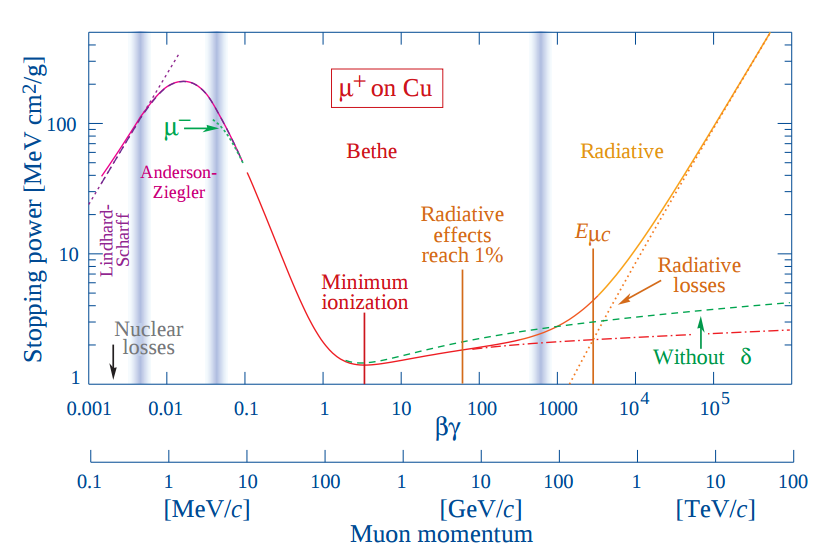
\includegraphics[width=0.95\textwidth]{bethe}
	\caption{Stopping power for positive muons in copper as a function of $\beta\gamma$. The solid curves show the total stopping power. The vertical lines show the range of validity of the curves \cite{pdg}.}
	\label{pbethe}
\end{figure}\no
This equation is valid in the energy range from $6\,$MeV up to $6\,$GeV or more generally $0.02 < \beta < 0.99$ within $1\,$\% accuracy. Below that limit the processes can be described by solid state physics and for higher energy Bremsstrahlung becomes dominant. The formula is completely independent of the mass of the traversing particle, the stopping power only depends on its speed and charge. By dividing by the density it becomes also almost independent of the target material. These facts demonstrate the universality of the equation.\\
In between the limits of the validity there are three prominent regions. For small $\beta\gamma$ the energy loss follows approximately $1/\beta^2$ until it reaches a broad minimum for $\beta\gamma \cong 3.5 $. A particle in this region is called \ac{MIP}. For larger $\beta\gamma$ the energy loss starts increasing again in a region referred to as logarithmic (or relativistic) rise.\\
Though not depending on the mass, the interacting particles still have to be a couple of orders of magnitude heavier than the electrons they are interacting with. That is why this formula does not apply to electrons or positron as incident particles. Their behaviour is shown in \ar{pelec}. For low energies the energy losses is mostly due to ionisation. For the most materials Bremsstrahlung becomes dominating above a critical energy of a few tens of MeV. A comparison between Bethe-Bloch and the stopping power for electrons is shown in \ar{pbetheall}.
\begin{figure}[ht]
	\centering
	\subbottom[Energy loss in lead as a function of electron or positron energy \cite{pdg}.]{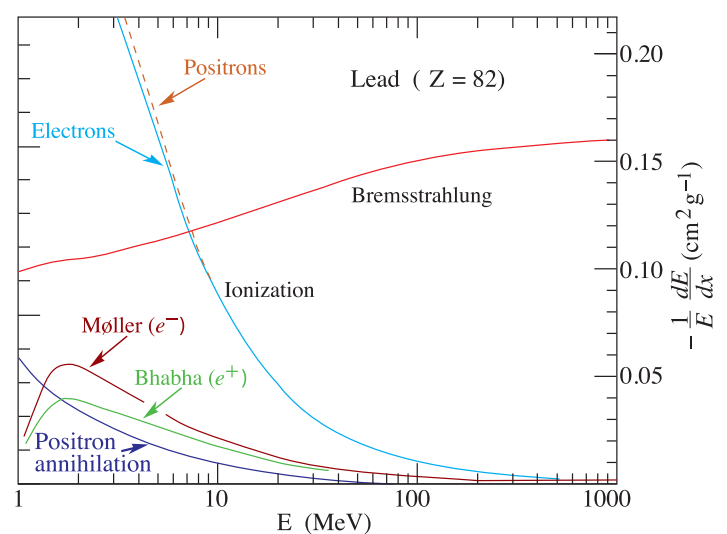
\includegraphics[width=0.47\textwidth]{elec}\label{pelec}}
	\hfill
	\subbottom[Energy loss for several positive particles in carbon \cite{murphy}.]{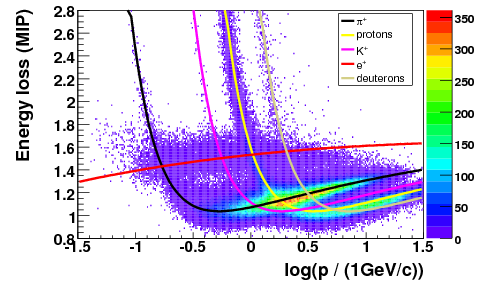
\includegraphics[width=0.47\textwidth]{betheall}\label{pbetheall}}
	\caption{Comparison of the stopping power of electrons/positrons and heavier charged particles.}
	\label{pcomp}
\end{figure}\no
% ========================================================
\subsection{Energy Loss Distribution}\label{slandau}
The Bethe-Bloch formula only describes the mean energy loss of a particle passing through matter. Since this is a statistical process the single values follow a certain distribution. For the material thickness of all utilised detectors during this thesis they follow a highly-skewed Landau (or Landau-Vavilov) distribution as shown in \ar{plan1}. If the thickness is increased the distribution gets less skewed as demonstrated in \ar{plan2} \cite{pdg}.
\begin{figure}[ht]
	\centering
	\subbottom[Electronic energy deposition distribution for a $10\,$GeV muon traversing $1.7\,$mm of silicon. $M0(\Delta)$ and $M1(\Delta)$ are the cumulative 0th moment (mean number of collisions) and 1st moment (mean energy loss) in crossing the silicon \cite{pdg}.\label{plan1}]{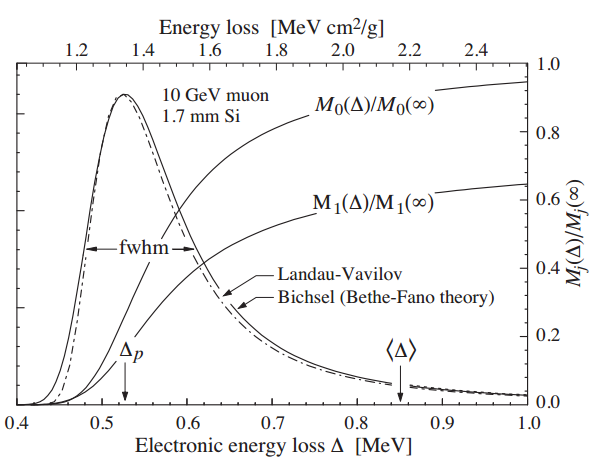
\includegraphics[width=0.47\textwidth]{landau1}}
	\hfill
	\subbottom[Normalised Straggling functions in silicon for $500\,$MeV pions. $w$ is the full width at half maximum \cite{pdg}.\label{plan2}]{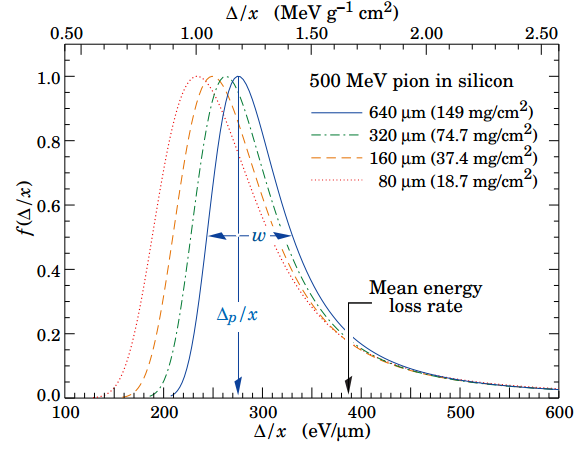
\includegraphics[width=0.47\textwidth]{landau2}}
	\caption{Distribution of the energy loss.}
	\label{plan}
\end{figure}\no
% ========================================================
% SEMICONDUCTOR DETECTORS
% ========================================================
\section{Semiconductor Detectors}
Semiconductor detectors are extensively used in particle physics to detect ionising particles. For the detectors used in this thesis it is important to get information about the spatial position of a particle and the amount of electrons created in the material. The most widely used semiconductor is silicon, which is also the material of the current tracking detector at \ac{CMS}. There are generally two different types of silicon tracker detectors: pixel and strip detectors, of which the former has a two dimensional and the latter has a one dimensional resolution. Using several layers of pixel or intersecting strip detectors (or a combination of both) achieves three dimensional reconstruction.\\
The working principle of a semiconductor detector is summarised in the following.
% ========================================================
\subsection{Semiconductor Basics}
A semiconductor is a material with an electric conductivity that lies between a conductor and an insulator. Responsible for that behaviour is their unique band structure, which is shown in \ar{pband}. The shell structure of the atoms in a bulk material consists of continuous energy bands of which two are responsible for the electric conductivity of the material: The highest band (in energy) that is completely occupied, the valence band, and the next highest band called conduction band. If an electron is lifted from the valence band to the conduction band, two charge carriers are created: the ``free'' electron in the conduction band and the electron ``hole'' in the valence band, which are called together an electron-hole pair.\\
Semiconductors are defined by the energy difference of the two bands that is called band gap energy. Semiconductors have band gaps that are smaller than about $4\,$eV and larger than $0.4\,$eV. A band gap of $0\,$eV would correspond to a metal and one above $4\,$eV to an insulator. This is the very behaviour that is exploited for particle detectors. If a particle traverses a semiconductor it looses energy due to ionisation as shown in \ar{sbethe} and thereby creates electron-hole pairs.
\begin{figure}[ht]
	\centering
	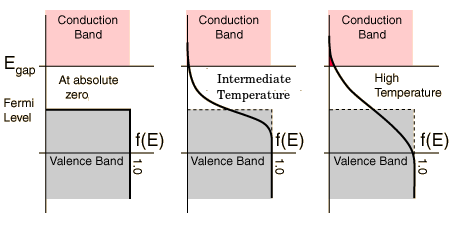
\includegraphics[width=0.6\textwidth]{band}
	\caption{Simplified band structure for a semiconductor at different temperatures. $f(E)$ denotes the Fermi distribution of the electron of the valence band. At temperatures above zero some electrons of the valence band have enough thermal energy to be lifted into the conduction band \cite{hyperphys}.}
	\label{pband}
\end{figure}\no
% ========================================================
\subsection{Signal to Noise}
As demonstrated in \ar{pband} the conductivity of semiconductors is temperature dependent due to the Fermi distributed electrons. Most semiconductors are already conductive at room temperature because some electrons have enough thermal energy to overcome the band gap. Using the Fermi distribution:
\begin{equation}
	f(E) = \frac{1}{1+e^{\frac{E-E_{f}}{kT} }}
\end{equation}
where $E_{f}$ refers to the Fermi energy, $T$ to the temperature and $k$ to the Boltzmann constant, the mean number of thermally created electron-hole pairs is about $3900$ per cubic millimetre at room temperature. Reading of \ar{plan2} the mean loss of energy for a \ac{MIP} is $1.65\,$MeV\,cm$^{2}$/g which corresponds for silicon with a density of $2.33\,$g/cm$^{3}$ to $3.84\,$MeV/cm. The average energy to produce an electron-hole pair is about $3.6\,$eV. Hence, the mean energy a \ac{MIP} loses in a silicon bulk with a thickness of $285\,\upmu$m equates to $30500$ electron-hole pairs. From this it follows that the thermal noise of a $12\,$cm strip detector of \ac{CMS} is of the same order of magnitude as the signal. For a \ac{CMS} pixel it is still around $5\,$\% of the signal. In order to conduct precise measurements, it is important to reduce the signal to noise ratio.
% ========================================================
\subsection{Doping \& pn-junction}
To overcome the free charge carriers at room temperature a reversed biased pn-junction is used, that fully depletes the silicon bulk.\\
All pure element semiconductors come from the carbon group because they have exactly four valence electrons and can either lose or gain electrons at the same time. There are two types of doping:
\begin{description}
	\item[n-type:]{Doping with elements from the nitrogen group (donor atoms, e.g. Arsenide or Phosphor) leads to an excess of loosely bound electrons in the lattice which shifts the Fermi energy closer to the conduction band.}
	\item[p-type:] Doping with elements from the boron group (acceptor atoms, e.g. Boron) leads to an excess of loosely bound holes in the lattice which shifts the Fermi energy closer to the valence band.
\end{description}
A pn-junction is created by bringing n-doped and p-doped semiconductors in contact with each other, which will cause a density gradient of the majority charge carriers across the junction. The electrons and holes wills diffuse into the opposite doped material and recombine to from a depletion zone with no free charge carriers. This results in a net movement of the electric charge and builds up an electric field across the junction until an equilibrium is established between diffusion and Coulomb force. 
% ========================================================
\subsection{Operation Mode}
If an external voltage is applied with the same polarity as the intrinsic potential barrier the depletion zone will increase; this is the process referred to as reverse biasing. In that way it is possible to deplete the whole bulk form charge carriers. Semiconductor detectors are usually operated over-depleted to be certain to create an electric field across the full detector volume. When a charged particle creates electron-hole pairs in that state, the charge carriers will drift to either side of the semiconductor parallel to the electric field and induce signals at the electrodes.\\
These are the very signals that are sent to the \ac{ROC} of the \ac{CMS} pixel detector (q.v. \ar{s130}) in order to detect these particles.
% ========================================================
% SCINTILLATORS
% ========================================================
\section{Scintillation Detectors}
\begin{figure}[ht]
	\centering
	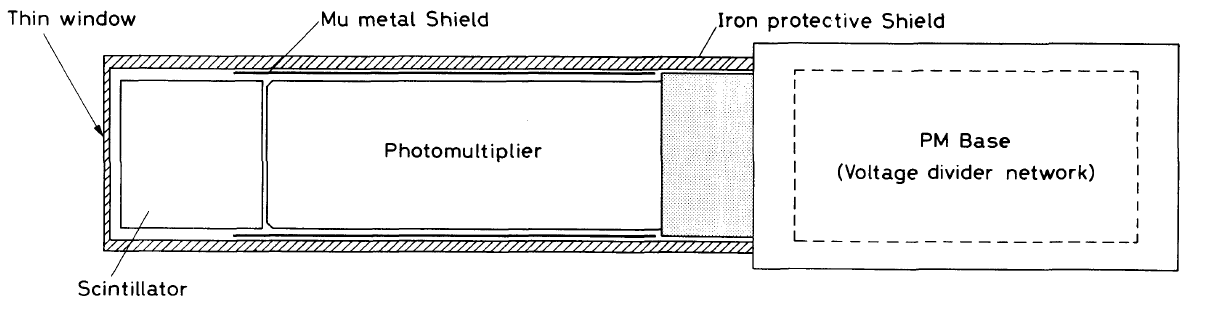
\includegraphics[width=0.94\textwidth]{scint}
	\caption{Schematic composition of a scintillation detector \cite{leo}.}
	\label{pscint}
\end{figure}\no
Scintillators belong to the most often and widely used particle detections devices in nuclear and particle physics. They make use of the property that some materials emit a short flash of light when hit by a nuclear particle or radiation. In the following the working principle of a scintillator will be sketched, for more information see \cite{leo}.\\
\ar{pscint} shows the basic elements of a scintillation detector. In general, it consists of a scintillating material that is optically coupled to a \ac{PM}, which either happens directly or via a light guide. Radiation or particles passing through the scintillator excite molecules and/or atoms which then causes the material to emit light. The light is guided to the the \ac{PM} where it is converted into a current by utilising the photoelectric effect. Thereupon the current is amplified by an electron multiplier, s.t. it is large enough to be measured. Depending on the material, scintillators provide some very useful features, e.g.:
\begin{itemize}
	\item sensitivity to the deposited energy
	\item fast time responses
	\item pulse shape discrimination (allows for particle identification)
\end{itemize}
Scintillation detectors exploit the so-called luminescence, which is the property to absorb incoming energy and re-emit it as light. If the re-emission happens within $10\,$ns, luminescence is called fluorescence. If it takes longer it is called phosphorescence. For scintillators only fluorescence serves. The time evolution of the re-emission follows an exponential decay of the excited states, which is split into two components as shown in \ar{pdecay}.\\
A viable scintillation detector has to meet the following requirements:
\begin{enumerate}
	\item a high conversion efficiency.
	\item transparency to the self emitted light.
	\item light emission in the spectral range of the \ac{PM}.
	\item a short decay constant.
\end{enumerate}
There are six different types of scintillating materials that split into organic and inorganic ) materials. The organic materials are either crystals, liquids or plastic and the inorganic materials are either crystals, gases or glasses.
\begin{figure}[ht]
	\centering
	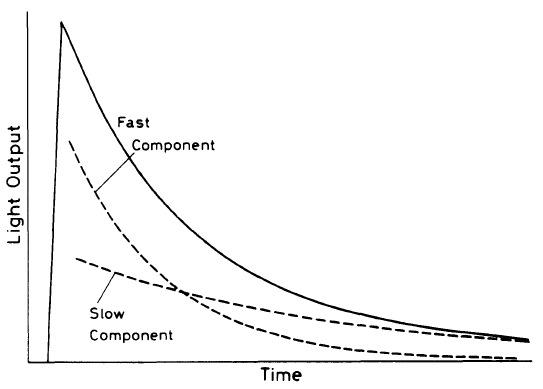
\includegraphics[width=0.5\textwidth]{decay}
	\caption{Exponential decay of fluorescent radiation with a prompt and a delayed component. The solid line corresponds to the total decay. \cite{leo}.}
	\label{pdecay}
\end{figure}\no
% ========================================================
% \subsection*{Plastic Scintillators}
% Plastic Scintillators are probably the most widely used organic detectors
% \begin{wrapfigure}{r}{4.5cm}
% 	\vspace*{-5pt}
% 	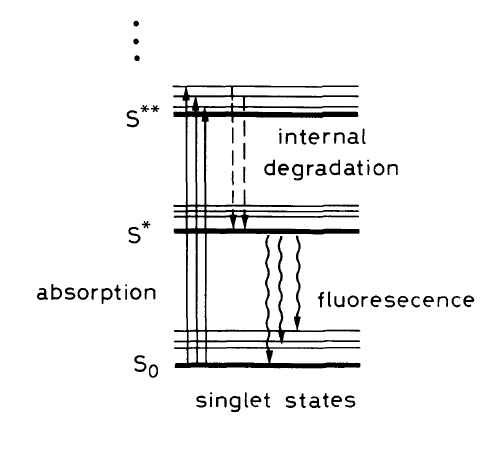
\includegraphics[width=4.4cm]{pimol}
% 	\caption{Energy level diagram of an organic scintillator molecule \cite{leo}}
% 	\label{ppimol}
% 	\vspace*{-5pt}
% \end{wrapfigure} 
% in particle physics due to their extremely fast signals of $2-3\,$ns and their good flexibility. They are a solution of organic scintillators in a solid plastic solvent like polyvinyl toluene, polyphenylbenzene or polystyrene. The solutions themselves are aromatic hydrocarbon compounds with a linked or condensed benzene ring structure. A typical example of an organic scintillator material is shown in \ar{ppbd}.\\
% The light in organic materials is produced by a transition of free valence electrons of the molecules where the delocalised electrons occupy $\uppi$-molecular orbits. An exemplary energy level diagram of that process is shown in \ar{ppimol}, where the ground state is singlet state $S_{0}$ with two excited electronic states $S^{*}$ and $S^{**}$ above. Each of the states has a fine structure due to vibrational modes. Penetrating radiation and particles excite both electron and vibrational levels (solid arrows) which generally decay immediately to $S^{*}$ (dashed arrows) without emission of light. $S^{*}$ in turn has a high probability to decay radiatively to one of the vibrational states of $S_{0}$ (waved arrows).This is causing the prompt component of the fluorescence, the delayed component originates from a triplet state with similar properties. The fact that $S^{*}$ decays to excited vibrational states of $S_{0}$ with a radiation energy less than $S_{0}$ $\rightarrow$ $S^{*}$ allows for the transparency to the own emitted light.\\
% \begin{figure}[ht]
% 	\centering
% 	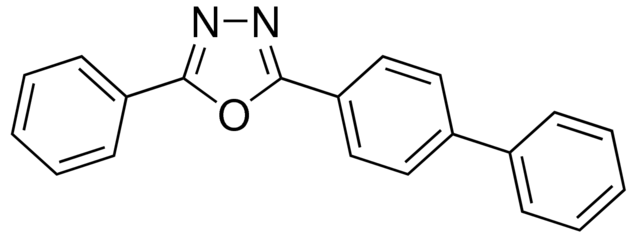
\includegraphics[width=0.5\textwidth]{pbd.png}
% 	\caption{2-(4-Biphenylyl)-5-phenyl-1,3,4-oxadiazole (PBD), \protect\chemfig{C_{20}H_{14}N_2O}.}
% 	\label{ppbd}
% \end{figure}\no
% ========================================================
% ELECTRONICS
% ========================================================
\section{Electronics}
In order to deliver the signals, to transform them or to build a trigger logic a lot electronics is required. Explaining every single device, which was used would go rather too far. Nevertheless it is quite important to possess knowledge about the two electronic standards NIM and \ac{TTL}.
% ========================================================
\subsection{NIM}
\begin{figure}[ht]
	\centering
	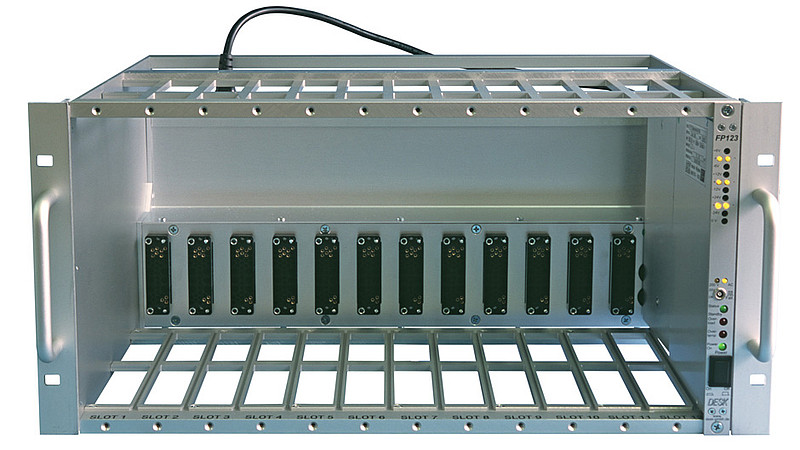
\includegraphics[width=0.95\textwidth]{nim}
	\caption{A standard NIM bin}
	\label{pnim}
\end{figure}\no
Initially NIM was an acronym for Nuclear Instrument Modules. However, as the use and manufacture spread farther throughout the world and it became truly international they were still identified with NIM. Having a company name as acronym was not appropriate any more and attempts to fit suitable words to the initials were in vain. So nowadays NIM only stands for NIM.\\
NIM is modular system and was the first and simplest standard established in particle physics. All basic apparatus, e.g. amplifiers, discriminators or scalers were designed in standard mechanical and electrical specifications. They fit into standardised so-called \textit{bins} that deliver the supply voltage via a rear plug of the device. Thereby it is very easy to build specific electronic system with many devices, like a trigger logic for example. They have an enormous flexibility.\\
The standard modules are $3.43\,$cm wide and have height of $22.2\,$cm  which also allows for multiples of that standard, i.e. double-width, triple-width, etc. A standard NIM fits $12$ single modules and is shown in \ar{pnim}.
% ========================================================
\subsection*{NIM Signals}
NIM include devices with both analogue and digital signals. The digital or logic signals have a fixed shape and only know the two states ON and OFF or equivalently 1 and 0.\\
There exist two types of standards called slow-positive and fast-negative. The latter one is referred to as NIM logic and has extremely fast rise times of the order of a nanosecond and a comparable width. The NIM logic levels are defined in \ar{tnim}. This definition is current based and all the input and output impedances are required to be $50\,\Upomega$. Fast-negative signal may be transported through long cables.
\begin{table}[ht]
	\centering
	\begin{tabular}{c|r c r|r c r!{\vrule width 2pt}r}
		\noalign{\hrule height 2pt}
				& \multicolumn{3}{c|}{\textbf{Output must deliver}} 	& \multicolumn{3}{c!{\vrule width 2pt}}{\textbf{Input must accept}} & \textbf{Voltage}							\\\hline
		Logic 1 & $-14\,$mA	&to	& $-18\,$mA							& $-12\,$mA	&to	& $-36\,$mA		& \multicolumn{1}{r}{$-0.8\,$V}	\\	
		Logic 0 & $-1\,$mA  &to	& $1\,$mA							& $-4\,$mA	&to	& $20\,$mA		& \multicolumn{1}{r}{$0\,$V}	\\
		\noalign{\hrule height 2pt}
	\end{tabular}
	\caption{Fast negative NIM logic. Neither rise time nor width are defined \cite{leo}.}
	\label{tnim}
\end{table}
% ========================================================
\subsection{\ac{TTL} Signals}
\ac{TTL} is no part of the NIM standard even though it is often used in particle physics. That is why this positive going logic is often found in NIM modules. Its levels are voltage based and can be found in \ar{tttl}.
\begin{table}[ht]
	\centering
	\begin{tabular}{c|r c r|r c r}
		\noalign{\hrule height 2pt}
				&  \multicolumn{3}{c|}{\textbf{Voltage}}							&  \multicolumn{3}{c}{\textbf{Corresp. current}}	\\\hline
		Logic 1	& $2\,$V	& $-$	& $5\,$V							& $40\,$mA	& $-$	& $100\,$mA				\\	
		Logic 0 & $0\,$V  	& $-$	& $0.8\,$V							& $0\,$mA	& $-$	& $16\,$mA				\\
		\noalign{\hrule height 2pt}
	\end{tabular}
	\caption{TTL signal levels \cite{leo}.}
	\label{tttl}
\end{table}
% ========================================================

\chapter{The CMS Pixel Chip}
% \tableofcontents
% ========================================================
% INTRO
% ========================================================
% Being a tiny part of the \ac{CMS} collaboration I would like to start by clarifying how my experiment is integrated into the amazing project called the \ac{LHC}.
% % ========================================================
% % LHC
% % ========================================================
% \section{\acf{LHC}}
% The LHC is the most powerful high energy particle accelerator that has ever been built on earth. The collider is located in a circular tunnel of $26659\,$m in circumference, which encloses an area of an area of $56.6\,$km$^{2}$ and partly underneath the territory of \ac{CERN}. It crosses the border between Switzerland and France and is close to the Swiss city Geneva. The accelerated particles are usually protons that are colliding with a \ac{COM} energy of $13\,$TeV \cite{lhc}, but there are also experiments with heavy ions.
% % ========================================================
% \subsection*{Accelerator Complex}
% In order to increase the energy of the protons from a few meV (kinetic energy) at room temperature up to $6.5\,$TeV a succession of machines is required. Each of these machines increases the energy successively and injects the protons into the next machine until it finally reaches the last iteration, the \ac{LHC}. A schematic of the whole process can be found in \ar{p18}.\\
% The protons are coming from an ordinary bottle of compressed hydrogen, whose molecules are stripped of their electrons in the source chamber of the linear accelerator LINAC2 which then accelerates them to $50\,$MeV using radiofrequency cavities. Having passed LINAC2, the particles are injected into the first circular accelerator, the \ac{PSB} where they are accelerated up to $1.4\,$GeV, which is already equivalent to $91.6\%$ of the speed of light. After that the \ac{PS} and the \ac{SPS} further increase their energy to $25$ respectively $450\,$GeV. Once the protons leave \ac{SPS} they are injected both clockwise and anti-clockwise into the two beam tubes of \ac{LHC} where they reach their final energy of $6.5\,$TeV within approximately $20$ minutes. Having $99.9999991\%$ of the speed of light the protons are now over $7000$ times heavier than the at rest.\\
% There are four major and two smaller experiments that use the \ac{LHC} as particle source: the two general purpose detectors \ac{CMS} and \ac{ATLAS}, a experiment designed for b-physics \ac{LHCb} and \ac{ALICE}, which is using heavy ions. The four major experiments are located in underground caverns around the interaction points. The \ac{LHCf} and a \ac{TOTEM} are the two smaller experiments; the first is one near \ac{ATLAS} and the latter close the interaction point of \ac{CMS}.
% \begin{figure}[ht]
% 	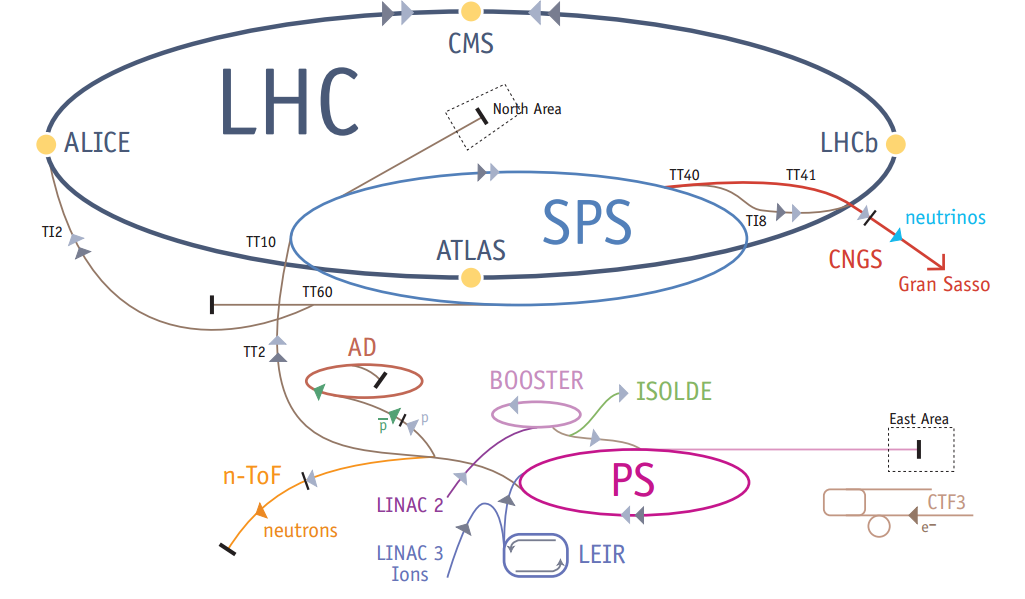
\includegraphics[width=0.95\textwidth]{lhc}
% 	\caption{Schematic of the \ac{LHC} accelerator complex \cite{lhc}.}
% 	\label{p18}
% \end{figure}
% % ========================================================
% % CMS
% % ========================================================
% \section{\acf{CMS}}
% \ac{CMS}, one of the general experiments at \ac{LHC}, is located beneath the French town Cessy. One of its main goals was the recent discovery of a new boson (assumed to be Higgs). Now the remaining  goals are the study of the properties of this boson and the search for evidence of physics beyond the Standard Model, in particular \ac{SUSY} and extra dimensions. The name \ac{CMS} derives from its design, which is rather small compared to other detectors of its capability (\ac{ATLAS}). \ac{CMS} has an excellent ability to measure myon tracks and a unique, very strong solenoid magnet.\\
% A sectional view of the whole detector is shown in \ar{p19}. It is set up in many shells of sub-detectors like layers of an onion. After the interaction, particles first pass the innermost detector, which is a tracker detector that measures i.a. the trajectory. After that comes an \ac{ECAL} and a \ac{HCAL} that measure the energy of the particles. The already mentioned sub-detectors are enclosed by the solenoid. The outermost layers outside of the coils consist of muon chamber. The \ac{CMS}-Pixel chip that is important for this thesis, is located in the innermost layer and is part of the tracker detector.
% \begin{figure}[ht]
% 	\centering
% 	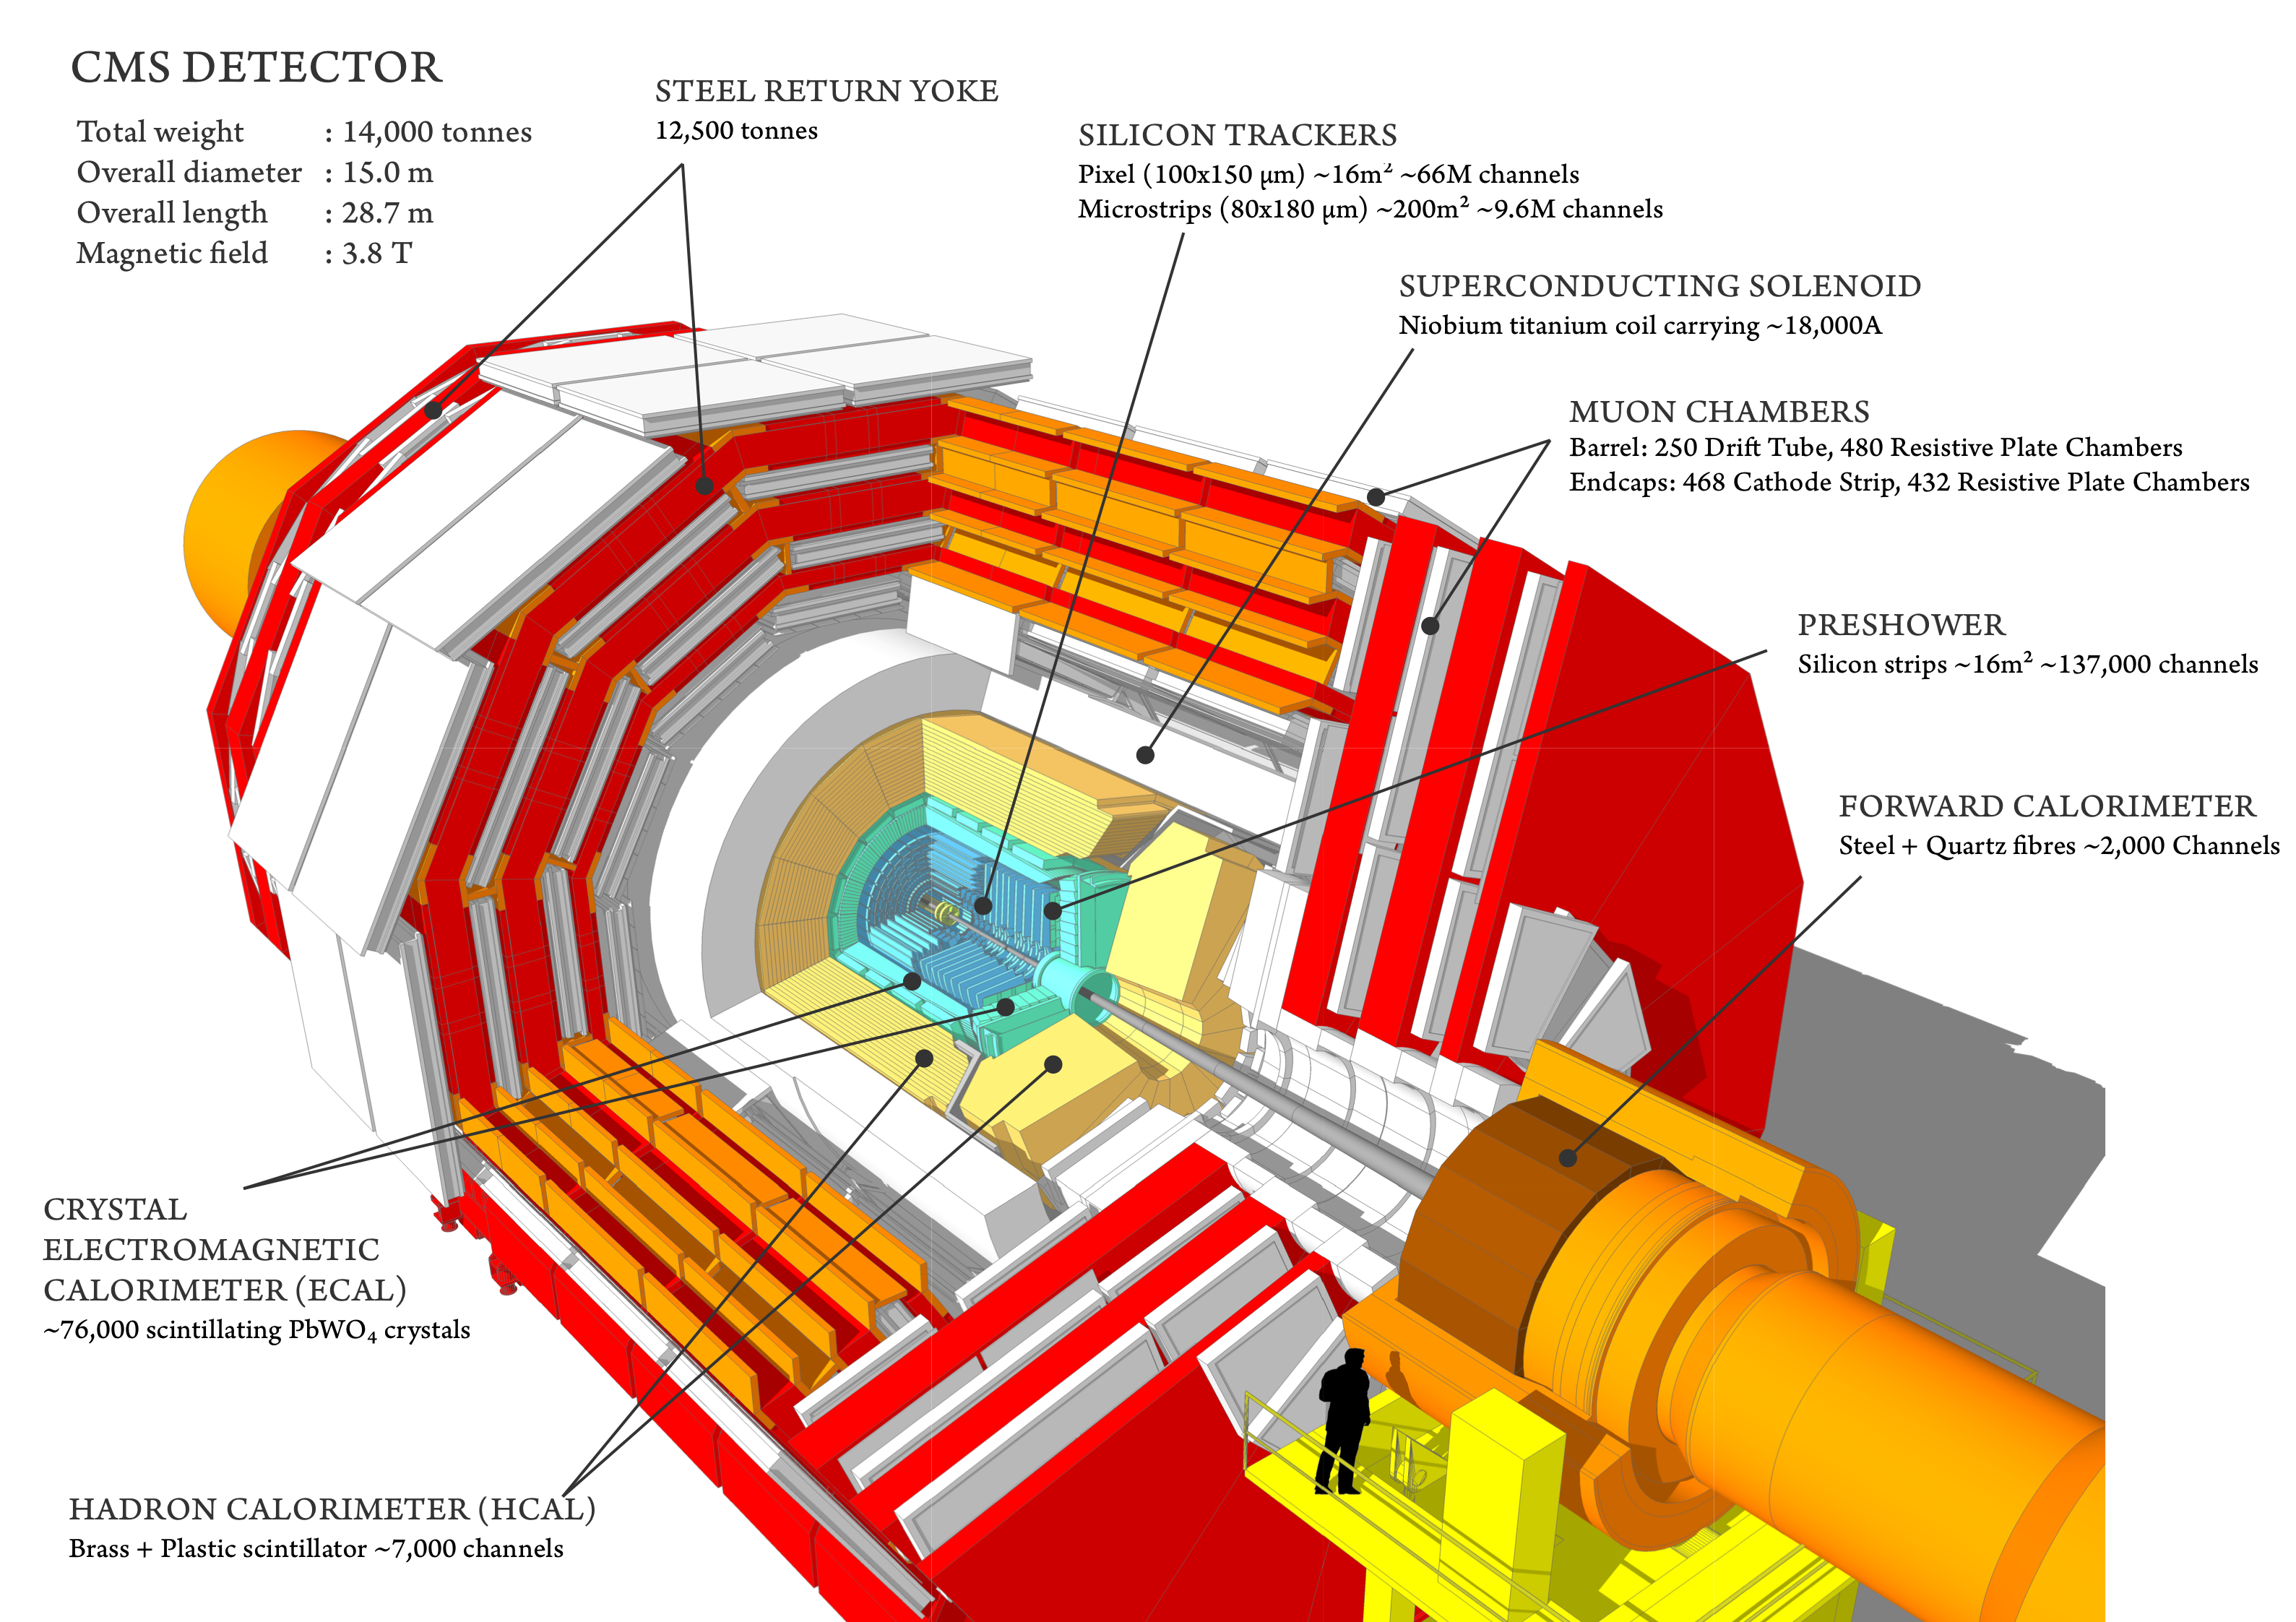
\includegraphics[width=0.95\textwidth]{cms_cut}
% 	\caption{Sectional view of the CMS detector \cite{cmsdet}.}
% 	\label{p19}
% \end{figure}
% % ========================================================
% \subsection{Solenoid}
% The shape of the solenoid strongly determines the whole design of the detector. A solenoid is a magnet of coils that are tightly wound into helices and have uniform magnetic field inside the helix, once constant electric current flows through the wires. Its purpose is to bend the paths of the particles that are created at the interaction point. It was aimed to be the strongest possible magnet since a stronger magnetic field leads to a smaller bending ratio of the particle gets and consequently increases the momentum resolution of the tracker. To reach a final magnetic field strength of $4\,$Tesla the whole magnet is cooled down to a temperature of $-268.5\,^{\circ}$C to guarantee superconductivity. Interestingly, particles with an energy of less than $1.6\,$GeV will circle inside the detector and will traverse to the end caps on a helical trajectory without ever reaching the calorimeter. 
% % ========================================================
% \subsection{Tracker Detector}
% The main goal of the tracker detector is to measure the momentum and the trajectory of passing particles to be able to get an idea of the incidents after the collision. The momentum is calculated using the circular trajectory of charged particles caused by the magnetic field. The \ac{CMS} tracker records the path of the charged particle by finding its position at a number of key points at each sub-layer of the detector. That way it is possible to precisely reconstruct paths of long living particles such as muons, electrons or hadrons, but also see the tracks of short living particles such as the beauty quark.\\
% For the whole experiment is very important to measure precise tracks on the one hand as well as to have as less disturbing\footnote{Less disturbing in that context means that the interactions of the Particles with the whole tracking detector has to be kept at a minimum.} of the particles as possible. That is one reason why only a certain number of points are measured for the tracking rather than than the maximum number. This was accomplished building $3$ layers of sub-tracker detectors around the beam line.\\
% The innermost layer of the detector is located but $4.4\,$cm away from the interaction point where the detectors are exposed to an approximate particle flux of $100\,$Mhz\,cm$^{-2}$. That is why the most important properties of the detector have to be radiation hardness and the ability to process a very high rate of events. When the current detector was built, it was decided to make it completely out of silicon. To be able to deal with the high number of particles the inner layers are made of pixel detectors whereas the outer ones, more than $20\,$cm away from the interaction point, are made out of strip detectors.
% % ==========================
% \subsubsection{Pixel Detector}
% Though only roughly the size of a shoe box, the Pixel Detector at \ac{CMS} contains $65$ million single pixels. They are arranged in three layers of barrel detectors $4.4\,$cm, $7.3\,$cm and $10.2\,$cm away from the beam and two forward detectors at either end (q.v. \ar{p22}). This system is able to reconstruct the tracks of ten million track per second and was build to withstand the duration for an operation time of ten years up to the Phase 1 Upgrade. Due to the huge amount of pixels it important keep the power consumption of the \ac{ROC}s at a minimum. Although they only need $50\,\upmu$W per pixel they are still mounted on cooling tubes so that the detector will not overheat. The cooling is also important reduce the electronic noise.\\
% The \ac{CMS} Pixel Detector is also the most important part concerning my thesis and is explained in further detail in \ar{s130}.
% \begin{figure}[ht]
% 	\centering
% 	\subbottom[\ac{CMS} silicon pixel detector \cite{cmsweb}.\label{p21}]{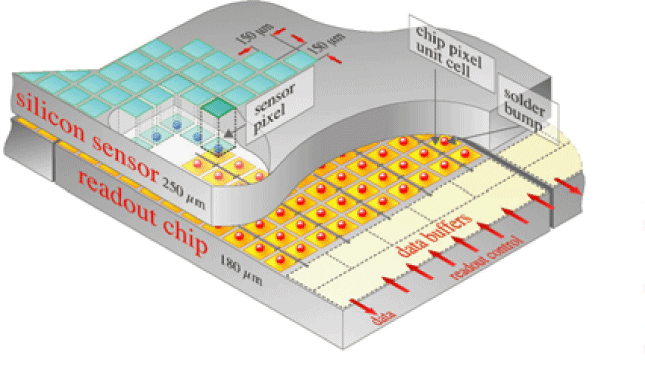
\includegraphics[width=0.47\textwidth]{pixelement}}
% 	\hfill
% 	\subbottom[Pixel layers around the beam line \cite{bora}.\label{p22}]{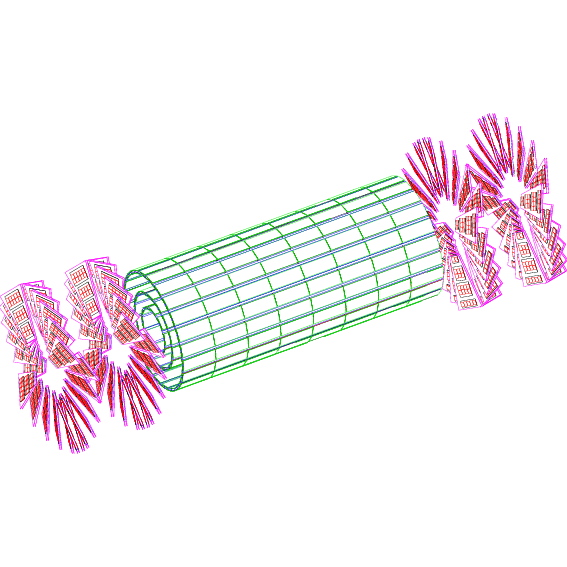
\includegraphics[width=0.47\textwidth]{barrel}}
% 	\caption{Schematics of the pixel detector.}
% 	\label{ppixdet}
% \end{figure}\no
% % ==========================
% \subsubsection{Strip Detector}
% Ten layers of strip detectors up to a radius of $130\,$cm surround the three pixel layers. A schematic of the way strip detectors are placed around the beam line is shown in \ar{p23}. First come four inner barrel layers with two inner endcaps. After them follow the outer layers: two double sided and four one sided barrel layers. Altogether the tracker detector consist of $10$ million silicon strips, which have the same working principle as the pixel detectors even though different chips are used for the readout. The whole system is also cooled down, in this case to a temperature of $-20\,^{\circ}$C.
% \begin{figure}[ht]
% 	\centering
% 	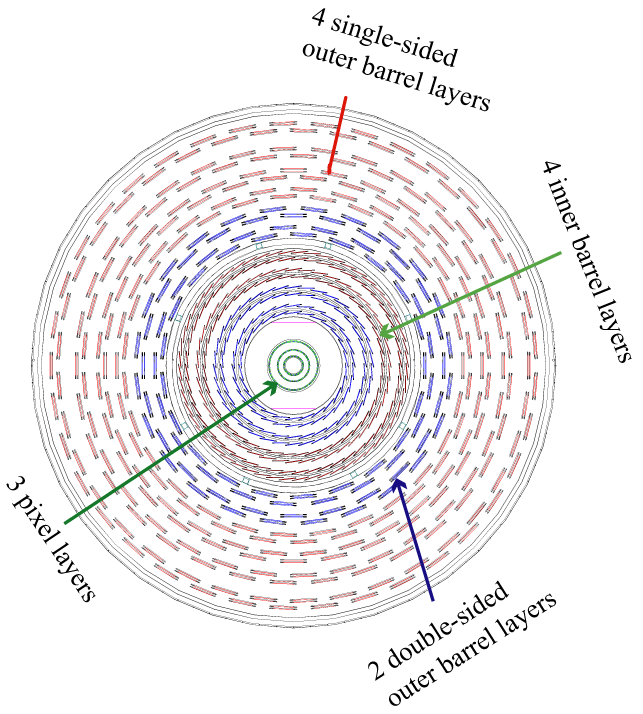
\includegraphics[width=0.4\textwidth]{strip}
% 	\caption{Tracker layers perpendicular to the beam \cite{cmsweb}.}
% 	\label{p23}
% \end{figure}
% % ========================================================
% \subsection{Calorimeter}
% In particle physics a calorimeter is a device to measure the energy of particles. When a particle enters the detector material a chain reaction called particle shower is started until the incident particle has deposited all its energy in the calorimeter. In many cases the detectors have transverse segmentation to provide information about the direction of the particle and longitudinal segmentation to get information about the identity of a particle by the shape of the shower. Since electrons and photons interact very differently with matter compared to hadrons, two different types of calorimeters are required: the \ac{ECAL} and the \ac{HCAL}.
% % ==========================
% \subsubsection{\ac{ECAL}}
% The \ac{ECAL} consists of $75848$ lead tungstate crystals (\chemfig{PbWO_{4}}), which is a scintillating material. With a short radiation length, narrow showers and a good radiation hardness \chemfig{PbWO_{4}} has excellent properties to function in such an environment. Glued on top of the crystals are photodetectors that collect the light, amplify it and transform it into into a electric signal, which then can be analysed.
% % ==========================
% \subsubsection{\ac{HCAL}}
% The \ac{HCAL} is built to measure hadrons which consist out of quarks and gluons. It was designed to be as hermetic as possible, i.e. to stop every particle from the collision in order to be able to draw conclusions about missing transverse energy. It is a so called sampling calorimeter which means that it finds the position, energy and arrival of a particle by using repeating layers of a dense brass absorber and plastic scintillators. This repeating architecture is also called sandwich structure. The \ac{HCAL} is the last part of the detector that is placed inside the solenoid.
% % ========================================================
% \subsection{Muon Chambers}
% Arranged on the outside of the solenoid are the muon chambers, since muons can even penetrate very dense material without losing a lot of energy. They are produced as decay products of many particles including potential new ones and thus play an import role as signals that can be triggered on. The whole muon detector consists of $1400$ muon chambers that split up into $250$ drift tubes and $540$ cathode strip chambers that track the particles and provide a trigger. The other part are $610$ resistive plate chambers that form a redundant trigger system, which decides weather to keep the data or not.
% % ========================================================
% \subsection{Examples}
% A diagram of all parts and the positioning within the \ac{CMS} detector is shown in \ar{p20}. It also demonstrates how typical particles will behave passing through the various steps. Photons and electrons are both stopped in the \ac{ECAL} but due to their charge electrons show a curved path in the tracker whereas photon tracks are straight. Charged hadrons will also leave a curved track and are generally stopped in the \ac{HCAL}. Because most myons are \ac{MIP}s they will not stop at all, but show a double curved track due the opposite magnetic field on the outside of the Solenoid.
% \begin{figure}[ht]
% 	\centering
% 	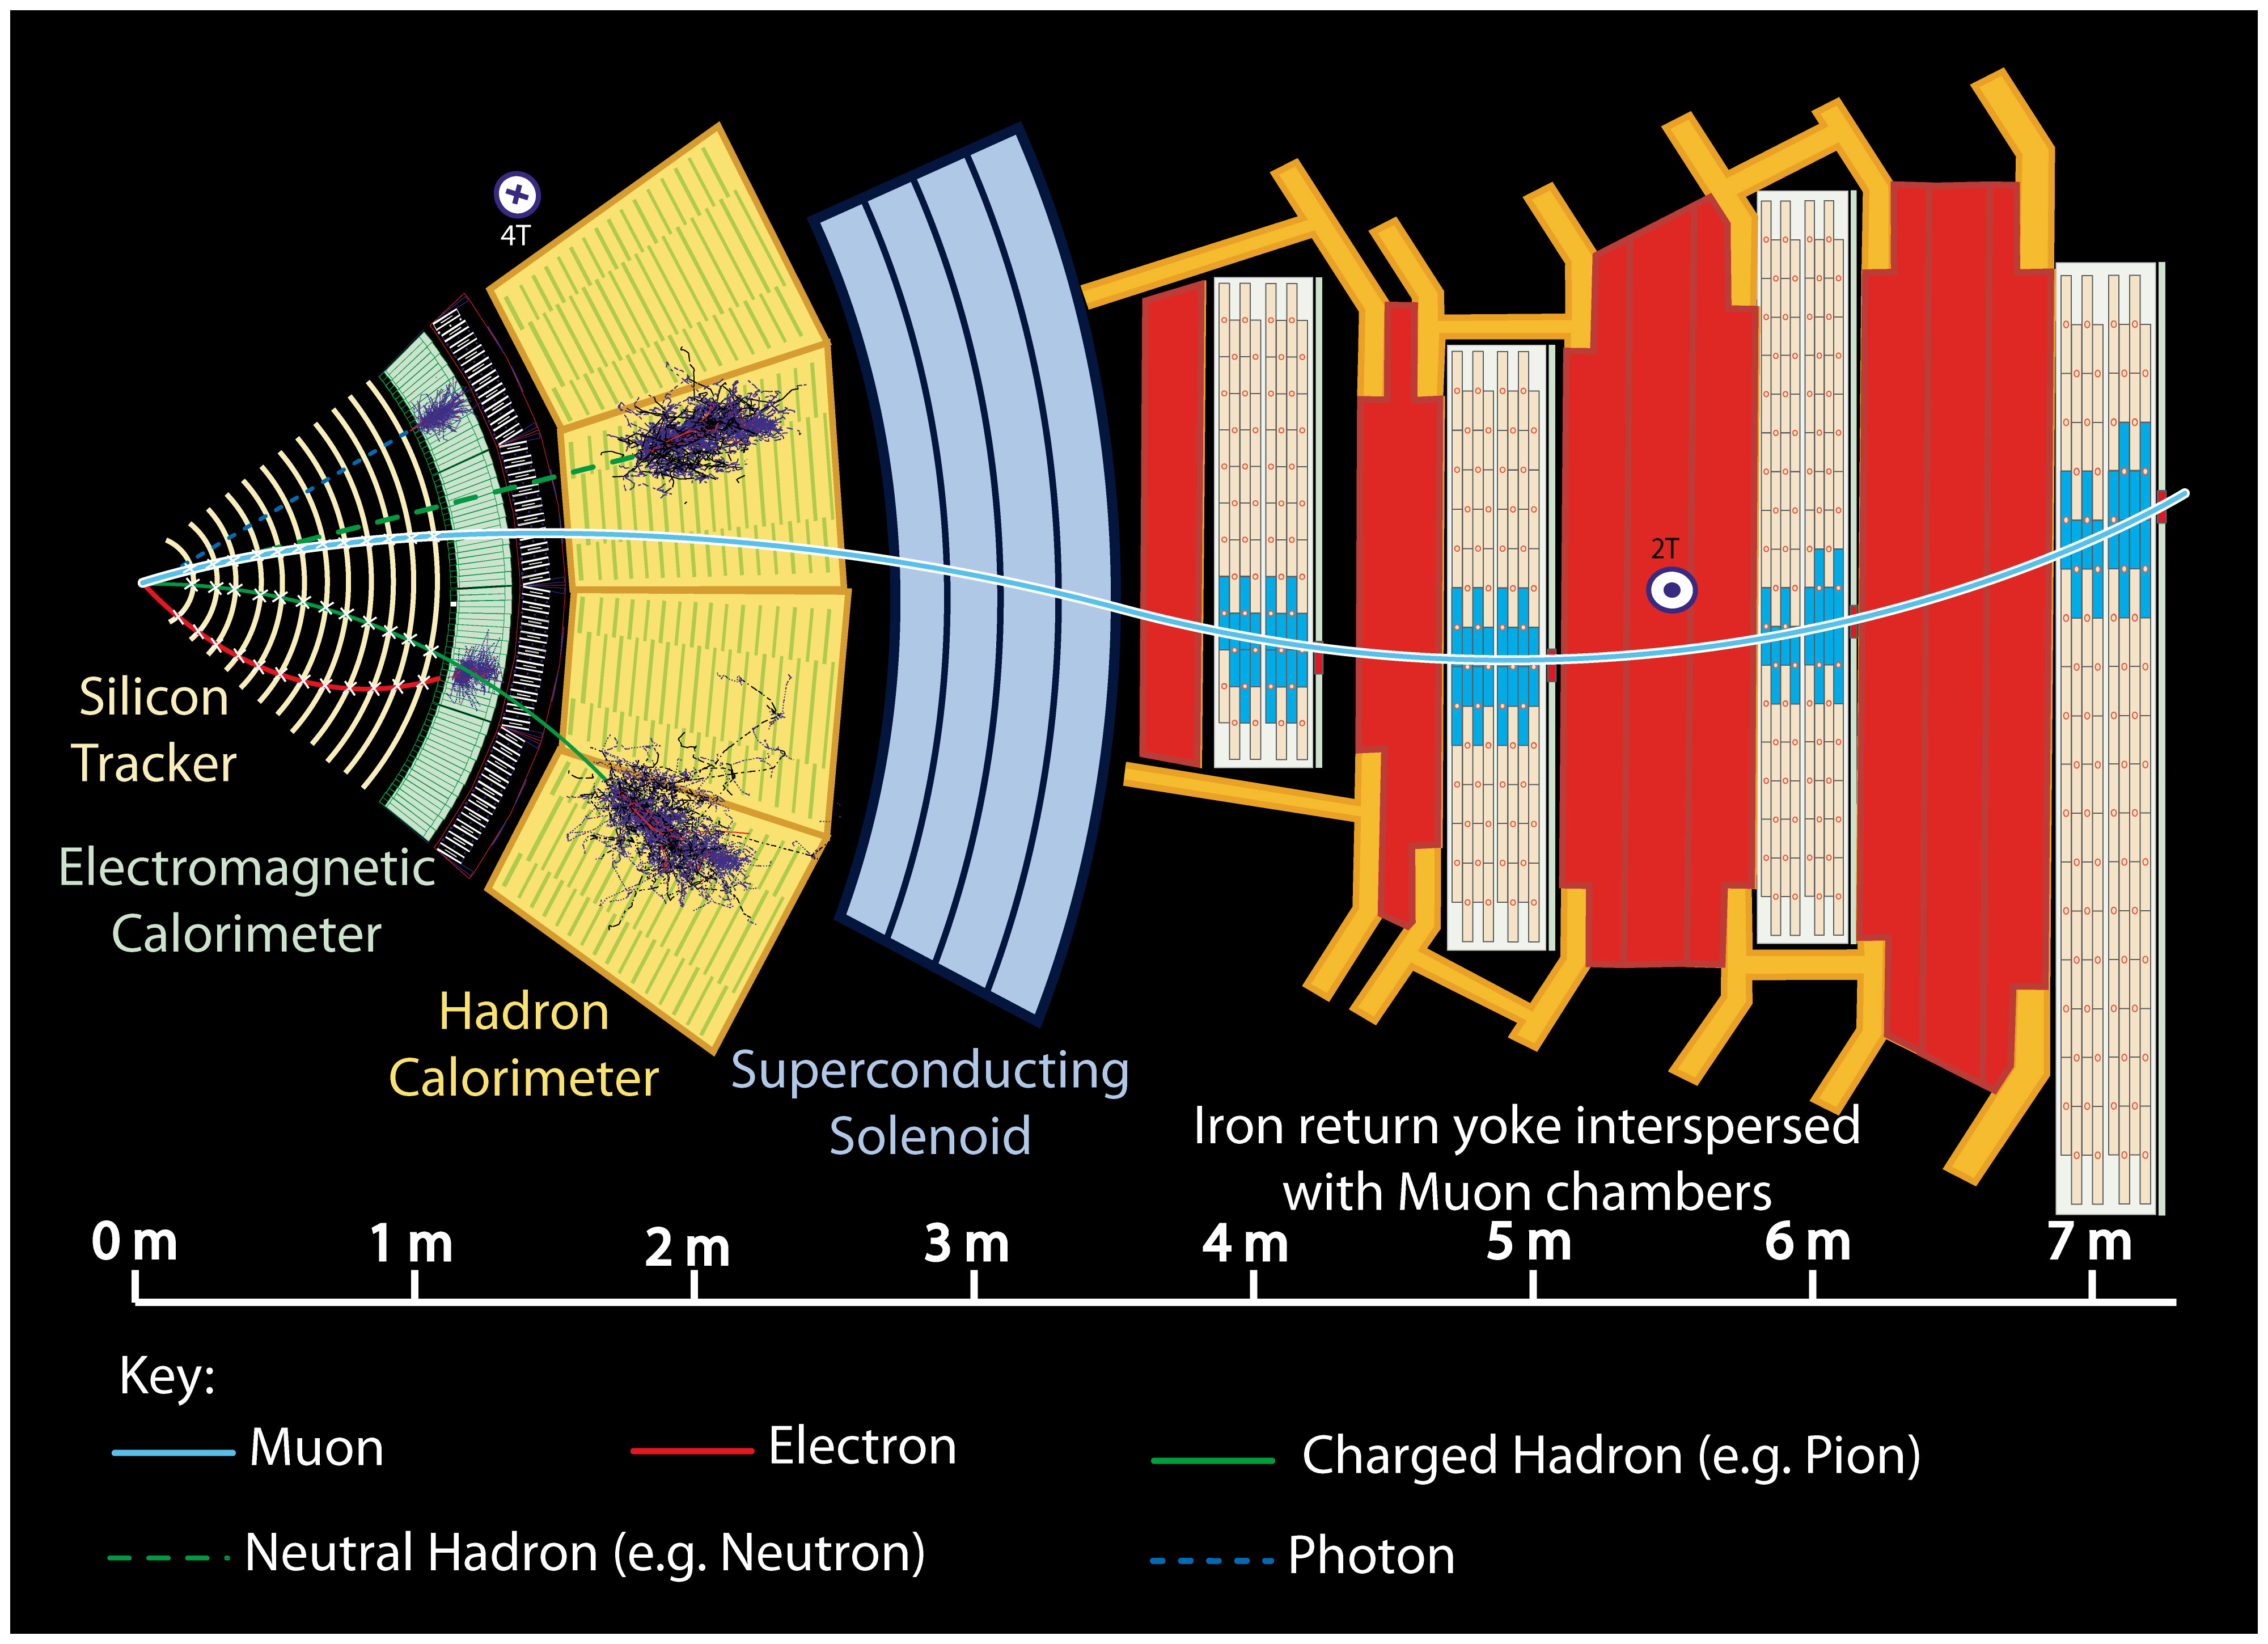
\includegraphics[width=0.95\textwidth]{cms_slice}
% 	\caption{Sliced view of the CMS detector with tracks of various particles \cite{cmsweb}.}
% 	\label{p20}
% \end{figure}
% % ========================================================
% \subsection{Trigger System}
% With almost a billion interactions per second\footnote{Roughly $20$ interactions per collision at a rate of $40\,$Mhz add up to a billion interactions} it is almost impossible to save or even analyse every single event. That is why a trigger system is required to save only the interesting events. Since there are collisions every $25\,$ns the data is stored in pipelines with precise timing information for a short time. In order not to mix up information from different events it is very important to synchronise the data streams. \\
% The first step to reduce the huge amount of information happens through the level 1 trigger, which is a full hardware trigger that decides within $3.2\,\upmu$s if the event could contain interesting physics based on information of the calorimeter and the muon chambers. These are events with large amount of energy or unusual combination of particles for example. The level 1 trigger selects $100\,$kHz of events out of the $1\,$GHz that are available. In the next step, the high level trigger, the whole event is recreated and the information sent to computers to pre-analyse it, which makes it a full software trigger. In the end only $100$ events per second are considered interesting and will be saved.\\ 
% The delays and the principle of the level 1 trigger of \ac{CMS} is important because it has direct connection to the trigger system used in the experiments concerning this thesis. 
% % ========================================================
% % CMS Pixel Chip
% % ========================================================
The CMS pixel chip is a tiny part of a detector of the world's most powerful high energy particle accelerator, the \ac{LHC}. It is utilised in the innermost layers of the tracker detector of \ac{CMS}, one of the two general purpose experiments at the \ac{CERN}. There it is essentially used to reconstruct particle tracks and measure the momenta of the charged particle using the tracks. The whole \ac{CMS} pixel detector is based on the pixel chip psi46v2 which has an analogue readout. During the Phase 1 Upgrade it is planned to exchange all of them with a more efficient digital silicon chip. It was also decided to add a fourth layer to the pixel detector. Due to the increase of the luminosity and \ac{COM} energy the Phase 2 Upgrade will require different materials for the innermost layers. A potential candidate are diamond pixel chips. Among other advantageous properties diamond is much more radiation resistant than silicon. Though, if diamonds are suited for that purpose is still under test.\\
During this thesis both analogue and digital silicon chips were used and there even was an opportunity to test digital diamond pixel chips. The purpose for the conducted experiments is in parts the exact same as for \ac{CMS}: use several \ac{ROC}s as tracking device. Additional applications will be described in the following.
% ========================================================
\section{Analogue Pixel Detector}\label{s130}
The analogue pixel detector was designed, inter alia, to precisely reconstruct hits, withstand radiation damage for several years of operation, keep multiple scattering at a minimum and avoid fake hits due to noise in electronics. Each single chip consists out of $4160$ pixels in $26$ double columns and $80$ rows. The single pixels have a size of $150\,\upmu$m $\times$ $100\,\upmu$m, which adds up to a total size of $7.8\,$mm $\times\ 8.0\,$mm (q.v. \ar{p24}) and corresponds to an area of a little more than half a square centimetre. The detector itself consists of two parts: a pixelated silicon sensor and a \ac{ROC}, which have both the same arrangement of pixels. The bump bonds are schematically shown in \ar{pbumpbonds} They are attached to one another and electrically connected via indium bump bonds of roughly $20\,\upmu$m in diameter \cite{kaestli}. The connection from the \ac{ROC} to the readout as well as the connection to the bias voltage is made via delicate wire-bonds.
\begin{figure}[ht]
	\centering
	\subbottom[Principle of a sensor bump bonded to the a chip \cite{dectris}.]{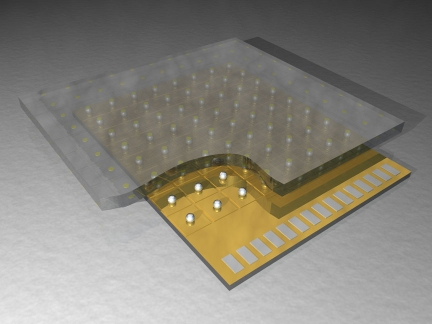
\includegraphics[width=0.47\textwidth]{bumpbonds}\label{pbumpbonds}}
	\hfill
	\subbottom[Photograph of an analogue pixel detector. The wire bonds are visible in the top right corner]{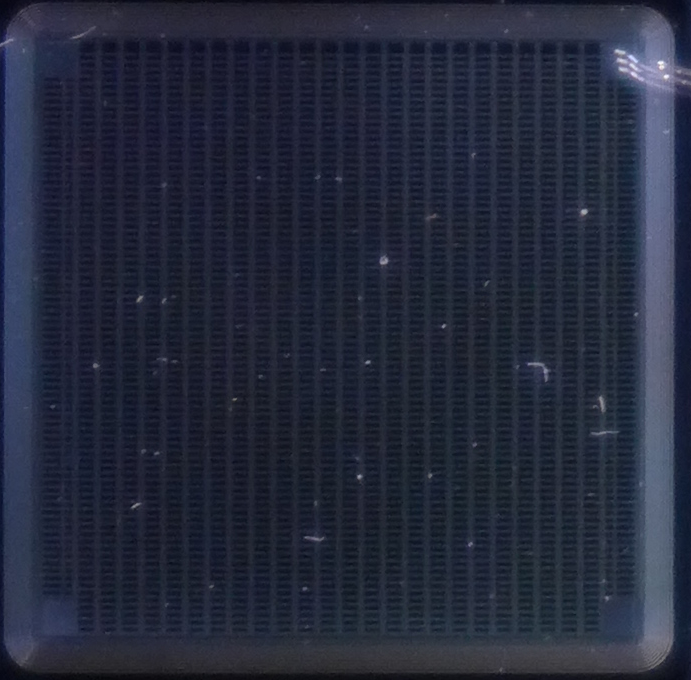
\includegraphics[width=0.47\textwidth]{ROC0}\label{p24}}
	\caption{Parts of the pixel detector.}
	\label{panaroc}
\end{figure}\no
% =======================
\subsection{Sensor}\label{s220}
For the current detector silicon was chosen as sensor material. The average energy to create an electron-hole pair in silicon is $3.6\,$eV. By applying a bias voltage to the sensor the charge carriers are moved to the collecting electrode and a signal can be measured. The silicon sensor itself consists of high-dose n-implanted pixels introduced into a high resistive n-substrate. The backside of the sensor is p-doped and thus creates a pn-junction \cite{allkofer}. The small pixel size was chosen to get a good spatial resolution. The thickness of the sensor is about $285\,\upmu$m so that minimum ionising particles will most probably create approximately $22000$ electron-hole pairs\footnote{The energy is loss is Landau distributed. This value is equivalent to the peak value of this distribution (q.v. \ar{slandau})} in the sensor. In order to fully deplete an unirradiated sensor of that thickness completely one has to apply a bias voltage of roughly $100\,$V \cite{pixadd}. For irradiated detectors that value may be a couple times higher, depending on the irradiation damage. 
% =======================
\subsection{\acs{ROC}}\label{sroc}
The \ac{ROC} has two parts: An active part consisting out of $26$ double columns of $2\times80$ \ac{PUC}s matching the pixels of the sensor and a periphery consisting of a control interface block, a data buffer, a time-stamp buffer and $35$ supply pads; this is depicted in \ar{p8}. All the signals going to and coming from the \ac{ROC} are put on these supply pads.\\
In order for the \ac{ROC} to record data, handle triggers and manage the readout, it also has four different counters:
\begin{enumerate}
	\item An $8\,$bit bunch crossing counter - whose information is sent to the time-stamp buffer,
	\item an $8\,$bit bunch crossing counter with trigger delay - runs a number of counts behind the bunch crossing counter (adjustable by the \ac{DAC} value wbc),
	\item an $4\,$bit trigger counter,
	\item an $4\,$bit token counter.
\end{enumerate}\par
The periphery is the reason is why the \ac{ROC} is with $7.9\,$mm$\times\ 9.8\,$mm 
\begin{wrapfigure}{l}{7.2cm}
	\vspace*{-10pt}
	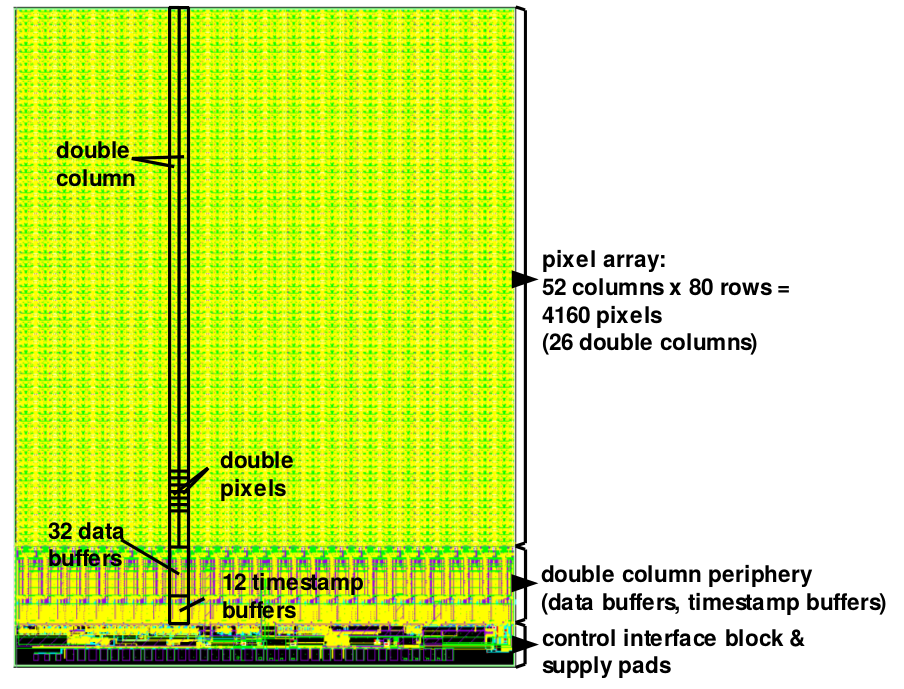
\includegraphics[width=7.2cm]{ROC_scheme}
	\caption{schematics of a \ac{ROC} \cite{psi46chip}}
	\label{p8}
	\vspace*{-5pt}
\end{wrapfigure}  
a few millimetres longer than the pixelated area of the sensor. The \ac{ROC} is programmable with a set of  $26$ \ac{DAC} values (q.v. \ar{t0}) that are required to control its behaviour. More details about the \ac{DAC}s can be found in \ar{sdacs}. The \ac{ROC} and its behaviour is temperature dependent, which is why it is also equipped with a temperature sensor.\\
If electron-hole pairs are created in the sensor, a voltage signal is induced in the corresponding \ac{PUC}. A schematic of a \ac{PUC} is shown in \ar{p9}. Once a signal enters the \ac{PUC} it gets amplified and shaped. If it exceeds a certain threshold, which is tunable with one the \ac{DAC}s, a signal is immediately sent to the periphery that will save the current bunch crossing into the time stamp buffer. The information of the hit (the \ac{PUC} address and the \ac{PH}) will be sent to a sample and hold capacitance until it is read out, which happens every $25\,$ns. Once read out, the data is stored in the data buffer.\\ 
There is an option to sent calibration signals directly to the front end of the \ac{PUC} that makes it very easy to test the basic functionality of the \ac{ROC} without requiring any particle hits. For every pixel the \ac{PUC} has a register to enable and disable sending these calibrates.\\
Furthermore, an important feature of the analogue \ac{ROC} is the so called fast-OR. Every time the threshold of a single pixel is exceeded, the \ac{ROC} sends out this signal. It is an logical OR of all pixels of the \ac{ROC} and its shape gives, inter alia, conclusions about the distribution of hit pixels (q.v. \ar{sfastor}). It is very important as trigger signal for other devices or as self trigger.
\begin{figure}[ht]
	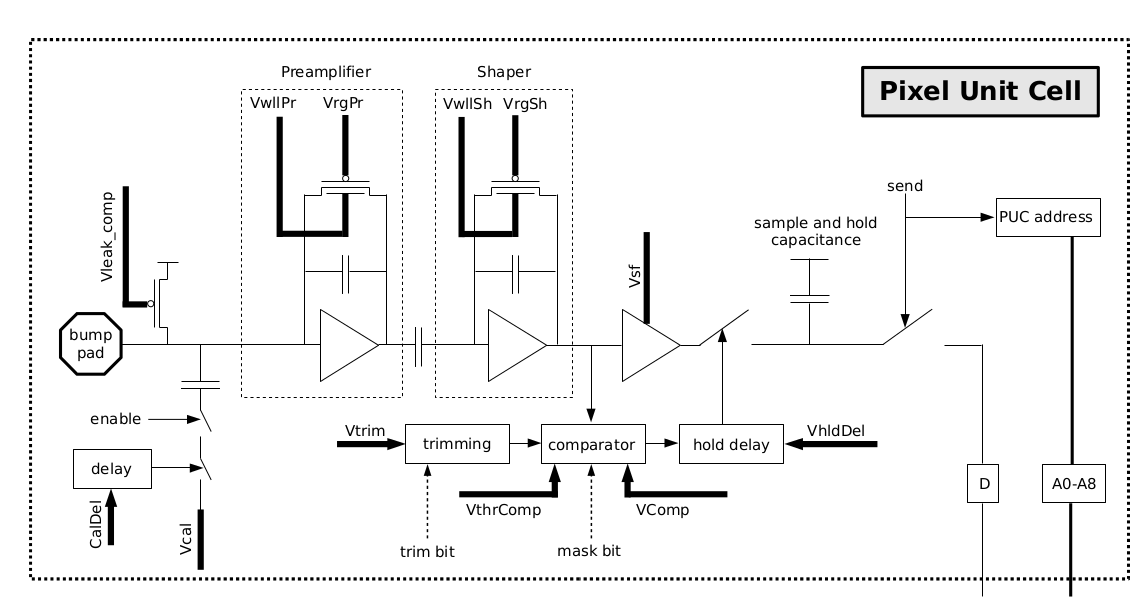
\includegraphics[width=0.95\textwidth]{PUC}
	\caption{Schematic view of a \ac{PUC} \cite{dambach}.}
	\label{p9}
\end{figure}
% =======================
\subsection{\acs{DAC}s}\label{sdacs}
An overview of all existing \ac{DAC}s for the analogue pixel chip with a short explanation is shown in \ar{t0} and \ar{t2}. In the following the most important \ac{DAC}s concerning this thesis are named.\\
In order to operate the chip it has to be supplied with a voltage. It was found that the chip is showing the best results while operating at a stable analogue current of $24\,$mA \cite{dambach}. This current can be adjusted by the $8\,$bit \ac{DAC} \textit{vana}. To be able to do basic tests with calibrate signals the correlation between \textit{vthrcomp} and \textit{caldel} has to be taken into account. It is only working in a certain region, which is explained in more detail in \ar{stornado}. Furthermore a common threshold for all pixels is of great importance. To achieve this a process called trimming is applied that exploits the inverse \ac{DAC} \textit{vthrcomp} and the \ac{DAC}s \textit{vcal} and \textit{vtrim}. More information about the trimming can be found in \ar{strim}. \textit{Vthrcomp} sets the global comparator threshold and \textit{vtrim} is responsible for the amount this global threshold can be lowered for each pixel. \textit{Vcal} regulates the amplitude of the calibrate signal and can be converted to the number of electrons created in the sensor. That is why it is also used to set a value for the common threshold.\\
Since for the undertaken experiments it was most important to have a stable fast-OR, \textit{vicolor}, \textit{vnpix} and \textit{vsumcol} were set in a way to have the maximum amplitude of the signal regardless of the shape. More details about the fast-OR and the effect of these \ac{DAC}s are in \ar{sfastor}.\\
\textit{Phoffset} and \textit{vcomp\_adc} can be used to adjust the address levels of the \ac{ROC}.
\begin{table}[ht]
	\begin{tabularx}{\textwidth}{c|l|X}
		\noalign{\hrule height 2pt}
		\textbf{\#} & \multicolumn{1}{c}{\textbf{Name(s)}} & \multicolumn{1}{|c}{\textbf{Explanation}}	\\\noalign{\hrule height 2pt}
		\multicolumn{3}{c}{\textbf{Voltage regulators}}														\\\hline
		$01$ & 	vdig				& sets the digital current 												\\\hline
		$02$ &	vana				& sets the analogue current 											\\\hline
		$03$ &  vsf // vsh			& influence on pulse height in low vcal range and digital current		\\\hline
		$04$ & 	vcomp				& regulates the supply voltage of the comparator						\\\noalign{\hrule height 2pt}
		\multicolumn{3}{c}{\textbf{Analogue Signal (\ac{PUC})}}												\\\hline
		$05$ &	vleak\_comp // vleak& controls leakage current 												\\\hline
		$06$ &	vrgpr				& \multirow{4}{7.6cm}{together control the pre-amplifier and the shaper and thereby the shape of the incoming signal}\\
		$07$ &	vwllpr				& 			 															\\
		$08$ &	vrgsh				& 																		\\
		$09$ &	vwllsh				&																		\\\hline
		$10$ &	vhlddel				& slightly influences the pulse height for different \textit{vcals} and pixels	\\\hline
		$11$ &	vtrim				& defines how much the trim bits for each pixel will increase the threshold\\\hline
		$12$ &	vthrcomp			& global comparator threshold											\\\noalign{\hrule height 2pt}
		\multicolumn{3}{c}{\textbf{Fast-OR Trigger (\ac{PUC})}}												\\\hline
		$22$ &	vicolor 			& \multirow{3}{7.6cm}{together define the shape of the fast-OR signal}		\\
		$23$ &	vnpix 				&  																		\\
		$24$ &	vsumcol	 			&  																		\\\noalign{\hrule height 2pt}
		\multicolumn{3}{c}{\textbf{Calibrate Signal (\ac{PUC})}}											\\\hline
		$22$ &	vcal	 			& sets the voltage for the calibrate signal (two ranges) 				\\\hline
		$22$ &	caldel	 			& delay of the calibrate signal											\\\noalign{\hrule height 2pt}
		\multicolumn{3}{c}{\textbf{Double Column Periphery}}												\\\hline
		$13$ &	vibias\_bus 		& switch for sending the address of the \ac{PUC} 						\\\hline
		$14$ &	vbias\_sf			& shifts the pulse height curve 										\\\hline
		$15$ &	voffsetop			& shift of pulse height  												\\\hline
		$16$ &	vibiasop			& switch for pulse height and influence of linear range 				\\\hline
		$17$ &	voffsetroc // phoffset	& switch for pulse height and influence of linear range 			\\\hline
		$18$ &	vion				& scaling of the pulse heights 											\\
		\noalign{\hrule height 2pt}
	\end{tabularx}					
	\caption{\ac{DAC}s of the pixel chip \cite{dambach}. Some \ac{DAC}s were renamed during the evolution of the chip which is why one \ac{DAC} can have several names.}
	\label{t0}
\end{table}\no
% =======================
\begin{table}[ht]
	\begin{tabularx}{\textwidth}{c|l|X}\noalign{\hrule height 2pt}
		\multicolumn{3}{c}{\textbf{Control and Interface Block}}											\\\hline
		$19$ &	ibias\_dac // vcomp\_adc	& scaling of the \ac{ROC} address levels and the pulse height 	\\\hline
		$20$ &	vibias\_ph // phscale& scaling of the pulse height 											\\\hline
		$21$ &	vibias\_roc 			& scaling of the \ac{ROC} address levels and the pulse height 		\\\noalign{\hrule height 2pt}
		\multicolumn{3}{c}{\textbf{Registers}}																\\\hline
		$253$ &	ctrlreg 			& switch between low and high vcal range (bit 2), full and half readout speed (bit 0) and on/off of the whole \ac{ROC} (bit 1)\\\hline
		$254$ &	wbc		 			& sets the bunch crossing at which the data will be read out 			\\\hline
		$255$ &	rangetemp 			& switch for different ranges of the temperature sensor  				\\\noalign{\hrule height 2pt}
	\end{tabularx}					
	\caption{\ac{DAC}s and Registers of the pixel chip \cite{dambach}}
	\label{t2}
\end{table}\no
% =======================
\subsection{Readout \& Trigger}\label{sread}
Each \ac{ROC} is set up to be read out in zero suppression mode, which means that only for pixel hits that exceed the threshold, the following information is sent to the periphery: The time stamp of the current bunch crossing is written into the time stamp buffer and the analogue signals are written into the next free data buffer. This process happens autonomously and asynchronously for every double column.\\
Concerning the readout of the \ac{ROC} two external signal lines are of importance: The \ac{CTR} and the token. As the name suggests, the former can send three kinds of information depending on the length of the pulse:
\begin{enumerate}
	\item a trigger signal, which is two clock cycles long.
	\item a calibrate signal, which is one clock cycle long.
	\item a reset signal, which is three clock cycle long.
\end{enumerate}
The information in the \ac{ROC} data buffer has to be kept until a potential trigger arrives. They are stored in the data buffer until one of the following events happens: 
\begin{itemize}
	\item The data was successfully read out by a connected device.
	\item The trigger window is exceeded (the bunch crossing counter passes the delayed time-stamp).
	\item The data buffer is full.
	\item A reset signal was received.
\end{itemize}
The process of the readout is described in the following: Hits that were sent to the periphery are validated by the external trigger signal by comparing their corresponding time stamps with the delayed bunch crossing counter. Non-validated hits are cleared. If the validation succeeds, the trigger counter is latched into the periphery, i.e. the double column is frozen and will not record further data until the information is read out or the \ac{ROC} receives a reset signal. Other double columns without validated hits remain active. When the latched trigger counter is matching the token counter the double column is set to readout mode and the trigger counter is incremented. As soon as the \ac{ROC} receives a token the frozen double columns are read out and reset. A token sent to the \ac{ROC} travels along the periphery consecutively reading out frozen \ac{DC}s. Just before the token leaves the periphery of a \ac{DC}, the token counter of that column is incremented as well. To every readout of the $26$ \ac{DC}s the \ac{ROC} also adds a header. Illustrations of the trigger validation and the readout procedure are shown in \ar{pro}.
\begin{figure}[ht]
	\centering
	\subbottom[Trigger validation.]{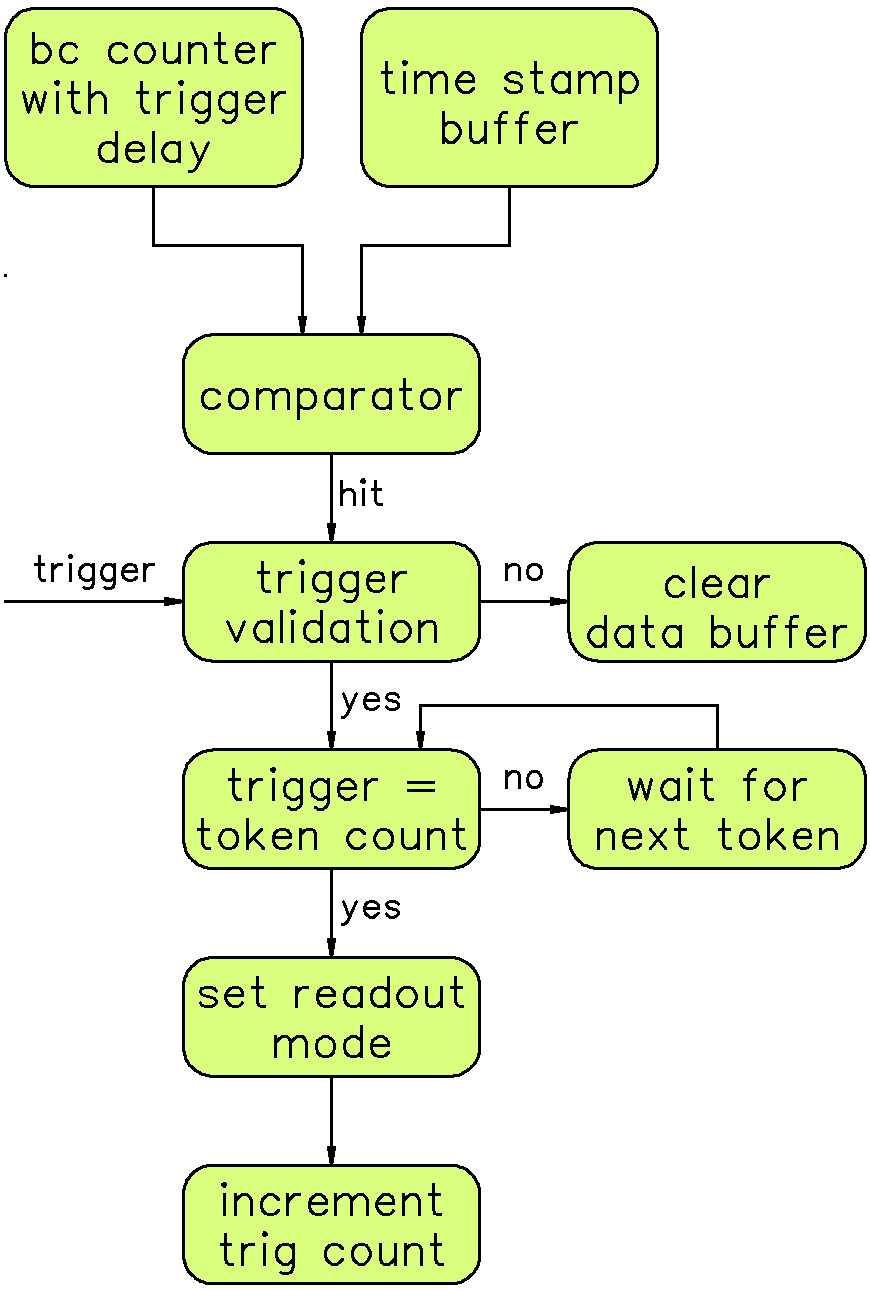
\includegraphics[width=0.37\textwidth]{trigger}\label{ptrig}}
	\hfill
	\subbottom[Readout procedure.]{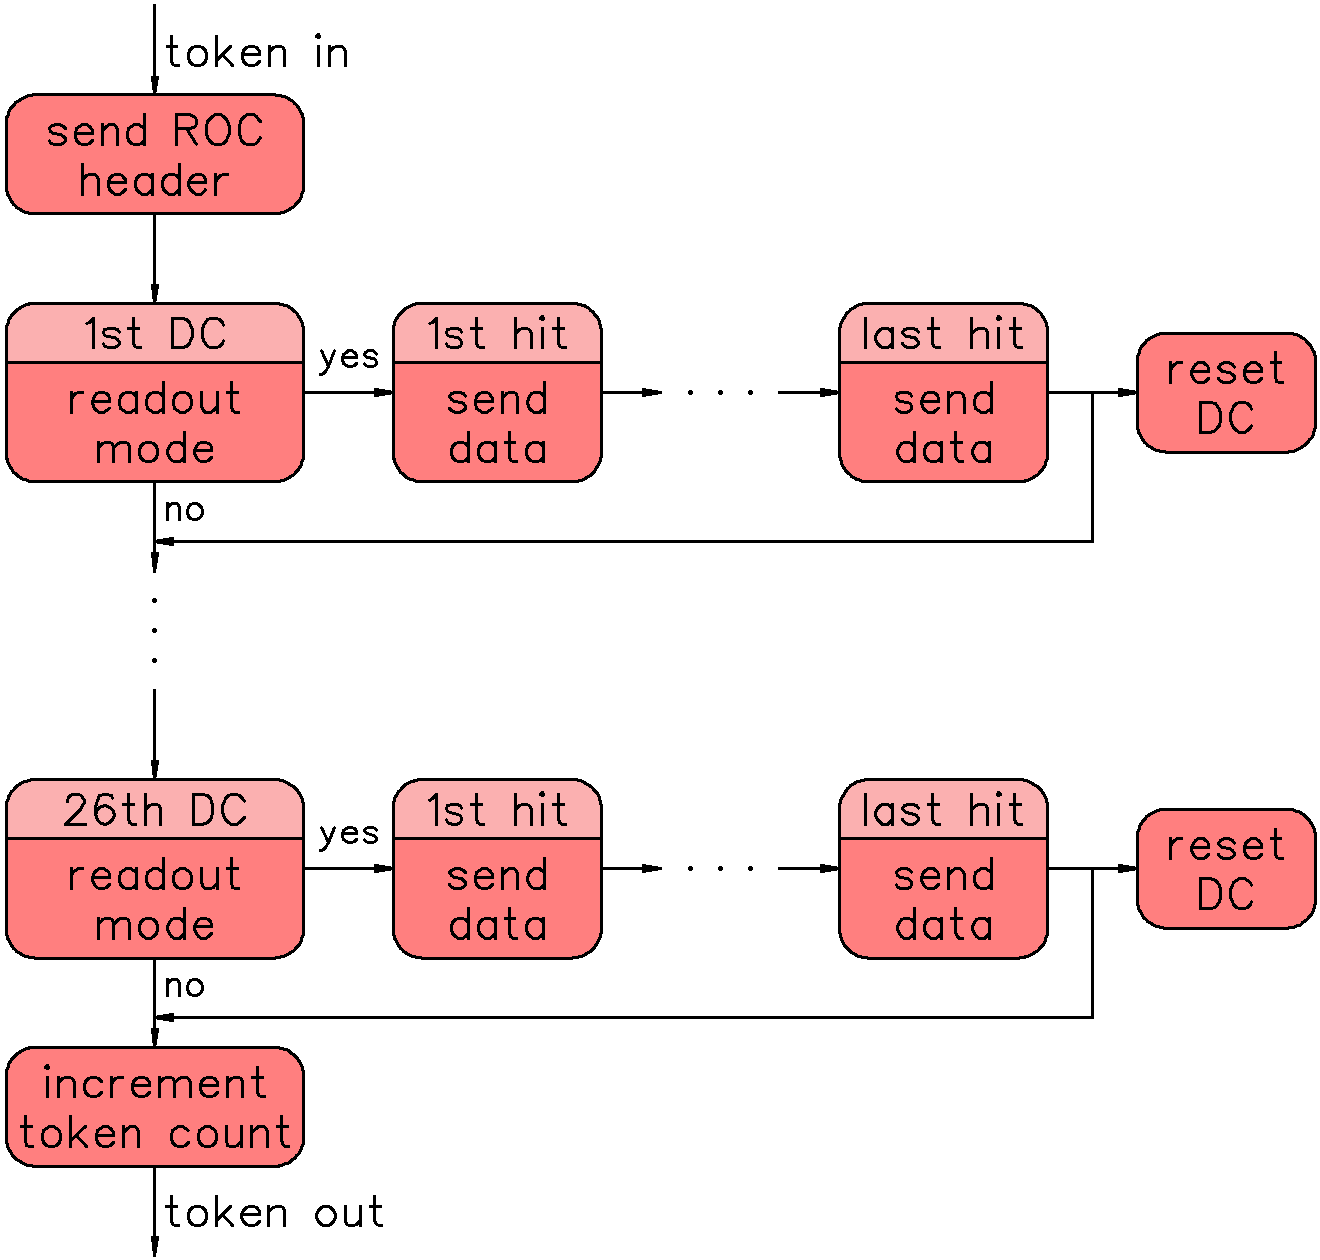
\includegraphics[width=0.57\textwidth]{token}\label{ptok}}
	\caption{Schematics of the readout of the \ac{ROC}. bc is short for bunch crossing and DC stands for double column}
	\label{pro}
\end{figure}\no
% =======================
\subsection{Data Format}\label{sdata}
An example of an analogue readout with only the information of the \ac{ROC} is shown in \ar{procsig}. The \ac{ROC} header is three clock cycles long. It contains an \ac{UB} level that is a very low, negative level and serves as reference, a \ac{B} level that is the zero reference of the differential signal and a level that is called \ac{LD}. The latter either points to the value the last \ac{DAC} was set to or the value of the temperature sensor of the chip. For every single pixel that was hit the \ac{ROC} will provide five levels containing the pixel address and one level with information about the pulse height. These six level are added to the header for each hit pixel. If no pixel was hit or the hits were not validated, the \ac{ROC} will send nothing but a header if a readout is started.\\
It is possible to read out several \ac{ROC}s with a single token. In that case the token is sent from one \ac{ROC} to the next collecting a header of each \ac{ROC} and the corresponding hit information s.t. a structure like header/hit/header/hit/hit/header/header/hit etc. will form. The readout concerning sending and handling trigger, reset and token is managed by a \ac{TBM}. For all the experiments described in the thesis the data was read with a \ac{DTB} that was developed at \ac{PSI}. The \ac{DTB} utilises a \ac{TBM} emulated on its \ac{FPGA} and is described in more detail in \ar{sdtb}.\\
\begin{figure}[ht]
	\centering
	\subbottom[Measured signal of several single pixel hits.\label{panasig}]{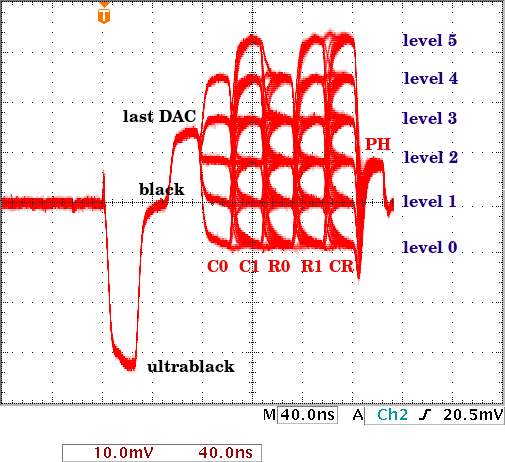
\includegraphics[width=0.47\textwidth]{siganalog}}
	\hfill
	\subbottom[Schematic signal of one single pixel hit.\label{p7}]{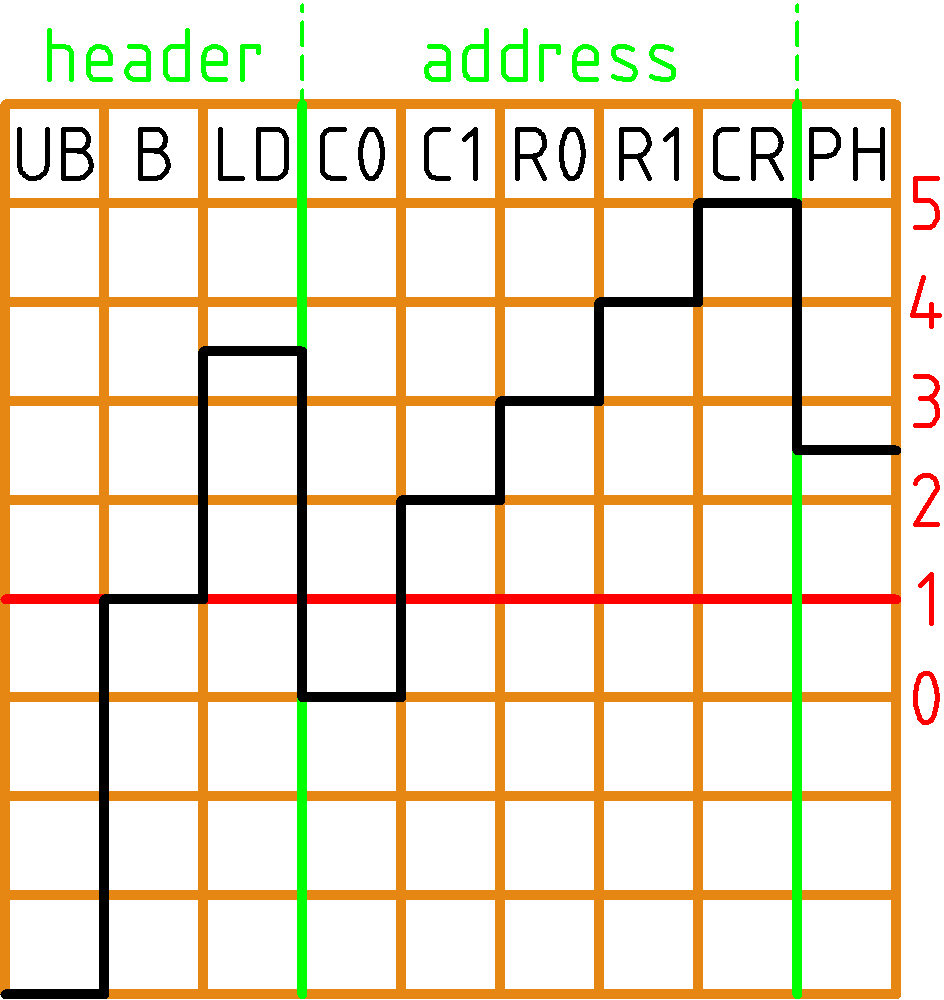
\includegraphics[width=0.47\textwidth]{levels}}
	\caption{Signals of the analogue \ac{ROC}}
	\label{procsig}
\end{figure}\no
% =======================
\subsubsection{\ac{I2C} Address}\label{si2c}
In order to be able to operate more than one \ac{ROC} with a single \ac{DTB}, every \ac{ROC} has a $4\,$bit \ac{I2C} address. The address can be set by connecting the supply pads $22-25$ to ground, of which each is equivalent to one bit. The bits are active if they are grounded, therefore the \ac{I2C} address is zero if none of the pads is connected. By sending commands to these addresses each \ac{ROC} can be programmed independently.
% =======================
\subsubsection{\ac{TBM}}\label{stbm}
\begin{figure}[ht]
	\centering
	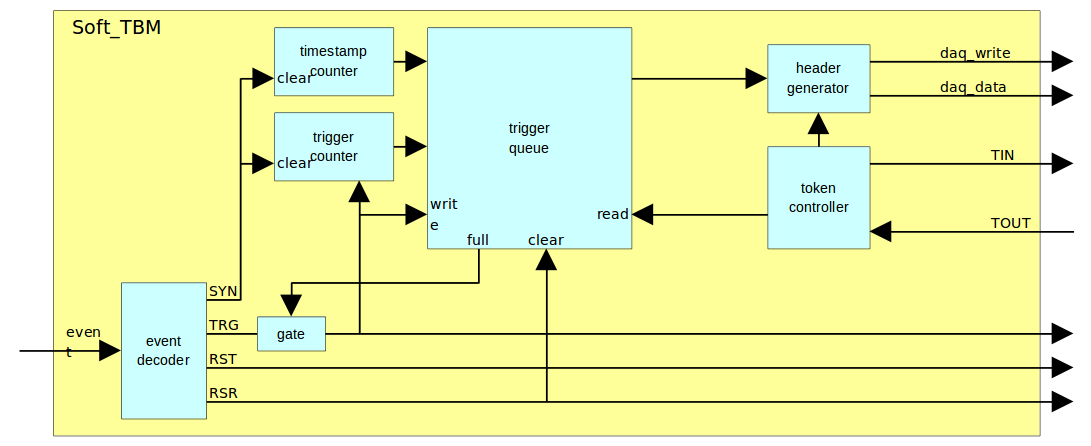
\includegraphics[width=0.95\textwidth]{tbm}
	\caption{Process chart of the emulated \ac{TBM}.}
	\label{ptbm}
\end{figure}\no
A process chart of the basic functionality of the \ac{DTB}'s \ac{TBM} is shown in \ar{ptbm}. While passing through the \ac{TBM} incoming triggers [TRG]  increment the $4./$bit trigger counter and write an entry into the trigger queue. This information is then read by the token controller, which sends out a token [TOUT] for each trigger and also receives the tokens [TIN] again that went to the \ac{ROC}. Once the token was received the the respective trigger gets cleared from the queue. The maximum amount of triggers in the trigger queue is $16$. If more triggers pile up until the [TIN] comes back, the triggers are caught by a gate where they are annihilated. There is also the possibility to clear the trigger queue with a reset signal. The token controller as well as the trigger queue send information to the header generator. When [TIN] arrives the header generator adds the information to the digital data stream in form of a header and a trailer, which each consist of two $16\,$ bit data words. The header contains an $8\,$bit event number and information about the trigger position inside the clock cycle.  The trailer contains, inter alia, a stack counter that is equivalent to the number of queued triggers. More information about the header and the trailer of the \ac{TBM} are given in \ar{stbmprob}. 
% ========================================================
\section{Digital Pixel Detector}\label{s23}
\begin{wrapfigure}{r}{4.5cm}
	\vspace*{-10pt}
	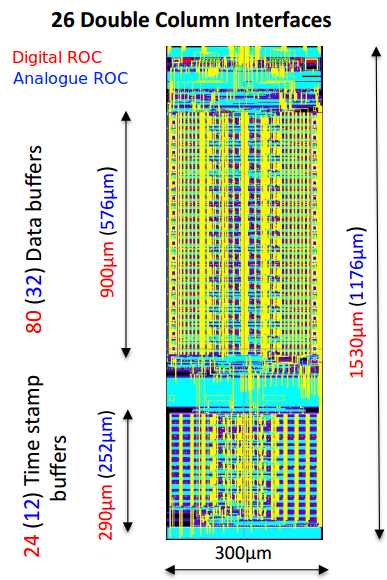
\includegraphics[width=4.4cm]{DigRocPeri}
	\caption{Double column interface of the digital \ac{ROC} \cite{hits}}
	\label{p12}
	\vspace*{-15pt}
\end{wrapfigure} 
For the Phase 1 Upgrade of \ac{CMS} a new digital \ac{ROC} was designed based on the analogue one. Their functionality is in principle still the same. An overview of the differences can be found in \ar{t3}.\\
One of the limitation of the analogue \ac{ROC} was a limited buffer size for the Level 1 trigger latency. To overcome this problem the number of data buffers was increased from $32$ to $80$. To reduce the readout related dead times due to higher rate, the number of time stamp buffers was doubled from $12$ to $24$. In addition the readout bandwidth had to be increased. This was done by switching to a fully digital readout by means of an on-chip \ac{ADC} for every \ac{DC}, new fast digital readout links, a \ac{PLL} to provide higher frequencies and some modifications to the control logic.An important feature of the new is the lower overall signal threshold that also increases the persistence of the chip \cite{hits}. This feature is indispensable for the low signals of diamonds, which is a possible candidate for a new generation of pixel chips. Going to lower thresholds was achieved by keeping the timewalk between the highest and lowest signal amplitudes within one clock cycle ($<16\,$ns) and reducing the cross talk in the digital \ac{ROC} layout as well as lower electronic noise. Besides, the output of the fast-Or signal was removed from the digital \ac{ROC}.\\
For easier usage the number of \ac{DAC} parameters is reduced to $16$. There is now only one parameter (\textit{vwllpr} and \textit{vwllsh}) for the pre-amplifier and the shaper instead of two and the leakage current compensation was removed. The six \ac{DAC}s for the double column periphery, which are responsible for the shape of the pulse height vs. \textit{vcal} curve, were condensed into \textit{vibias\_bus} and \textit{phoffset}. A comparison of the \ac{DAC}s that changed can be found in \ar{tdacchange}.
\begin{table}[ht]
	\centering
	\begin{tabularx}{0.85\textwidth}{X|l|l}\noalign{\hrule height 2pt}
			 &\multicolumn{1}{c}{\textbf{psi46v2}}	&\multicolumn{1}{|c}{\textbf{psi46dig}}	\\\hline
		\ac{ROC} size					& $7.9\times9.8\,$mm	& $7.9\times10.2\,$mm 	\\
		Pixel size						& $100\times150\,\upmu$m& $100\times150\,\upmu$m\\
		Smallest radius					& $4.3\,$cm				& $2.9\,$cm				\\
		\ac{DAC}s / registers			& $26$ / $3$			& $16$ / $3$			\\
		Power up condition				& not defined			& default values		\\
		Pixel charge readout			& analogue				& digitised, $8\,$bit	\\
		Readout speed					& $40\,$MHz				& $160\,$Mbit/s			\\
		Time stamp buffer size			& $12$					& $24$					\\
		Data buffer size				& $32$					& $80$					\\
		Output buffer FIFO				& no					& yes					\\
		Double column speed				& $20\,$MHz				& $40\,$MHz				\\
		Metal layers					& $5$					& $6$					\\
		leakage current compensation	& yes					& no					\\
		In-time threshold				& $3500\,$e				& $<2000\,$e			\\
		\ac{PLL}						& no					& yes					\\
		Data loss at max 				& $\sim3.8\,$\% at  	& $\sim3\,$\% at		\\
		operating flux					& $120\,$Mhz/cm$^{2}$	& $580\,$Mhz/cm$^{2}$ \footnotemark[2]\\\noalign{\hrule height 2pt}
	\end{tabularx}					
	\caption{comparison between analogue and digital \ac{ROC} \cite{hits}}
	\label{t3}
\end{table}\no
\footnotetext[2]{This is valid for the layer 1 version of the digital chip, that is planned for the Phase 1 Upgrade.}
\begin{table}[ht]
	\begin{tabularx}{\textwidth}{c|l|l|X}
		\noalign{\hrule height 2pt}
		\textbf{\#} & \multicolumn{1}{l}{\textbf{analogue}} & \multicolumn{1}{|l}{\textbf{digital}}	& \multicolumn{1}{|l}{\textbf{comment}}\\\noalign{\hrule height 2pt}
		\multicolumn{4}{c}{\textbf{Analogue Signal (\ac{PUC})}}							\\\hline
		$05$ &	vleak				& $-$ 		& leakage current compensation removed			\\
		$06$ &	vrgpr				& $-$ 		& combined into vwllpr		\\	
		$07$ &	vwllpr				& vwllpr	&							\\
		$08$ &	vrgsh				& $-$		& combined into vwllsh		\\
		$09$ &	vwllsh				& vwllsh	&							\\\noalign{\hrule height 2pt}
		\multicolumn{4}{c}{\textbf{Double Column Periphery}}				\\\hline
		$13$ &	vibias\_bus 		& vibias\_bus	&						\\
		$14$ &	vbias\_sf			& $-$			&						\\
		$15$ &	voffsetop			& $-$			& the six periphery dacs\\
		$16$ &	vibiasop			& $-$			& were condensed into two \\
		$17$ &	voffsetroc			& phoffset		& 						\\
		$18$ &	vion				& $-$			&						\\\noalign{\hrule height 2pt}
		\multicolumn{4}{c}{\textbf{Control and Interface Block}}			\\\hline
		$19$ &	vibias\_dac 		& vcomp\_adc 	&						\\
		$20$ &	vibias\_ph 			& phscale 		& 						\\
		$21$ &	vibias\_roc 		& $-$			& removed				\\\noalign{\hrule height 2pt}
		\multicolumn{4}{c}{\textbf{Fast-OR Trigger (\ac{PUC})}}				\\\hline
		$22$ &	vicolor 			& vicolor	&							\\
		$23$ &	vnpix 				& $-$		& fast-OR removed			\\
		$24$ &	vsumcol	 			& $-$		& fast-OR removed			\\
		\noalign{\hrule height 2pt}
	\end{tabularx}					
	\caption{Different \ac{DAC}s for analogue and digital \ac{ROC}}
	\label{tdacchange}
\end{table}\no
% ========================================================
\section{Digital Test Board}\label{sdtb}
The psi46 \ac{DTB} is the interconnect between a computer and the \ac{ROC}. In the past the analogue chips were operated with an \ac{ATB}, which has some major disadvantages in comparison with the \ac{DTB}. For example it has only a limited amount of data it can save, s.t. during beam tests one could only take runs of $300000$ events until the buffer was full. One of the achievements of this thesis is the possibility to reliably operate analogue chips as well as digital chips with the \ac{DTB}.\\
The \ac{DTB} is powered by a $6\,$V AC to DC power supply and connects via an adapter to the \ac{ROC}. It has two interfaces to a computer of which the ethernet is not implemented yet, leaving the USB 2.0 as only option. In here lies another advantage compared to the \ac{ATB}, which only had a USB 1.1 connection: The writing speed is increased a lot. In order to use several \ac{DTB}s on the same computer, each \ac{DTB} has its own serial number. Once connected to the chip and a computer, the \ac{DTB} and its \ac{FPGA} are completely controlled with a software called pXar. The \ac{FPGA}, which is emulating the \ac{TBM}, has its own firmware developed at \ac{PSI}. By now there more than twenty iterations of this firmware, which can be easily upgraded via USB. During this thesis the firmware versions from $4.0$ to $4.2$ were utilised.\\
It is possible to read out several signals of the \ac{DTB}. For that purpose there are two digital and two differential analogue LEMO outputs.\\
Furthermore the \ac{DTB} has inputs for an external clock and trigger, which accept \ac{TTL} signals. The height of the external trigger signal has to be at least $3\,$V to guarantee stability. Since these inputs are not terminated, it is very important to terminate incoming signals at the input to avoid reflections inside the cables. The \ac{DTB} also has a \ac{HV} input that is able to distribute the \ac{HV} to the sensor.
\begin{figure}[ht]
	\centering
	\subbottom[Top view.]{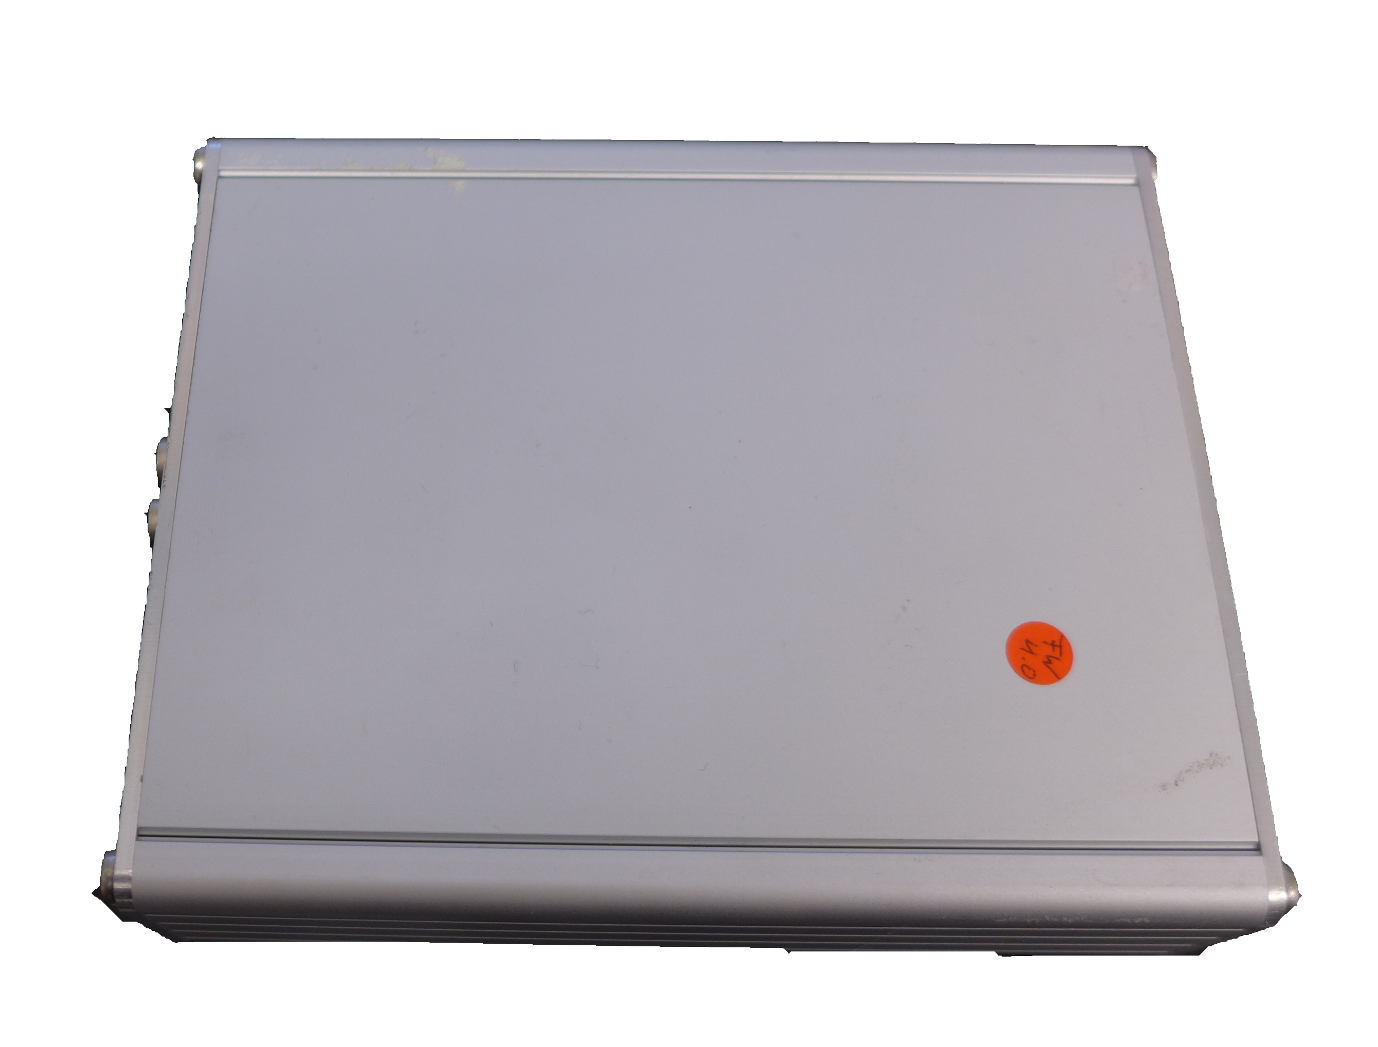
\includegraphics[width=0.47\textwidth]{DTB}\label{p10}}
	\hfill
	\subbottom[Front and backside.]{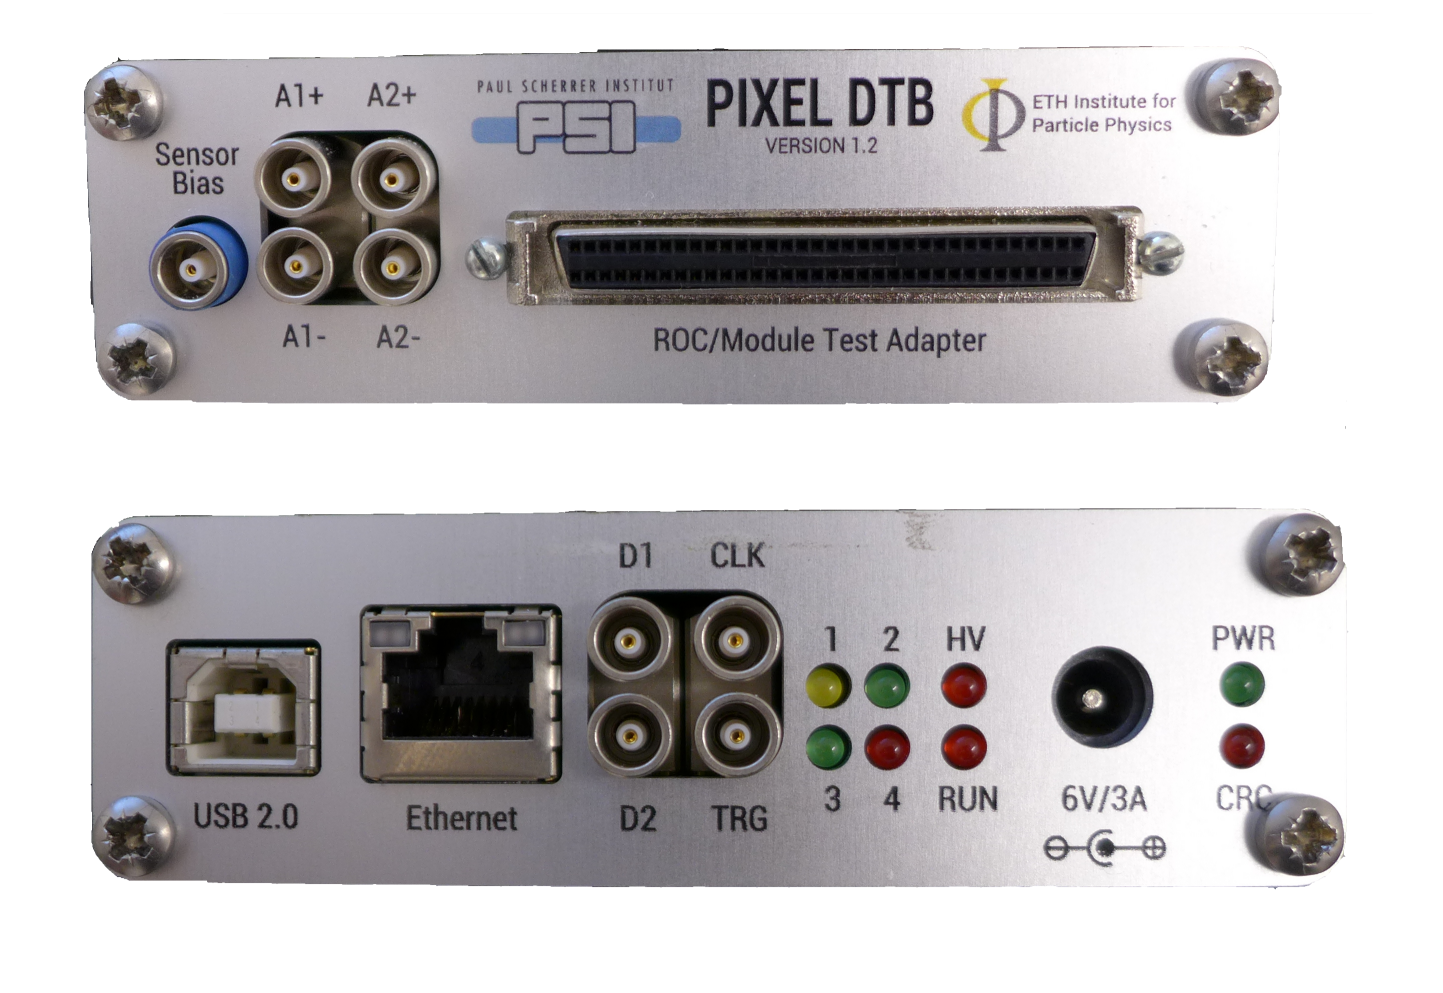
\includegraphics[width=0.47\textwidth]{DTB-Sides}\label{p11}}
	\caption{Photographs of the \ac{DTB}.}
	\label{pdtb}
\end{figure}\no
% ========================================================

\chapter{The Foundation of the Experiment - Telescope}
% ========================================================
% INTRO
% ========================================================
\section{Introduction}\label{s20}
The Compact Pixel Tracking Telescope has two different versions that were both constructed at \ac{ETH} in Z{\"u}rich. It is called telescope due to the fact that it utilises different single planes to get information about a \ac{DUT}. Its main purpose is to provide an event trigger and high resolution tracks.\\ 
To accomplish that goal it consists of several single \ac{CMS}-Pixel chips that are placed consecutively, perpendiclar to the beam. The chips are mounted on so-called adapter planes and have a fixed distance to one another that is given by the connectors of the connectors of the motherboard.\\
The planes are daisy chained and are read out by the \ac{DTB} which makes them accessible via a computer.
% ========================================================
% 1
% ========================================================
\section{Telescope Layout}\label{s21}
As already mentioned above, there are two versions of the telescope. Version 1 was designed to be as simple as possible and consists of six planes with analogue chips. Whereas the second version that was built on the experience with first one, comprises three plane modules, which may be combined to bigger modules. The modules of version 2 can consist either of digital chips or of analogue chips. Version 2 has some additional features as well that will be mentioned in the following.\\
Both consist mainly of three parts: a motherboard, adapter planes and the \ac{ROC}s.
% ========================================================
\subsection{Motherboard}\label{s210}
The motherboard is the main frame of the telescope. Pictures of the motherboards are shown in \ar{pmb}, the number in square bracket in the following text refer to the numbers in the pictures.\par
\begin{figure}[h]
	\centering
	\subbottom[Version 1]{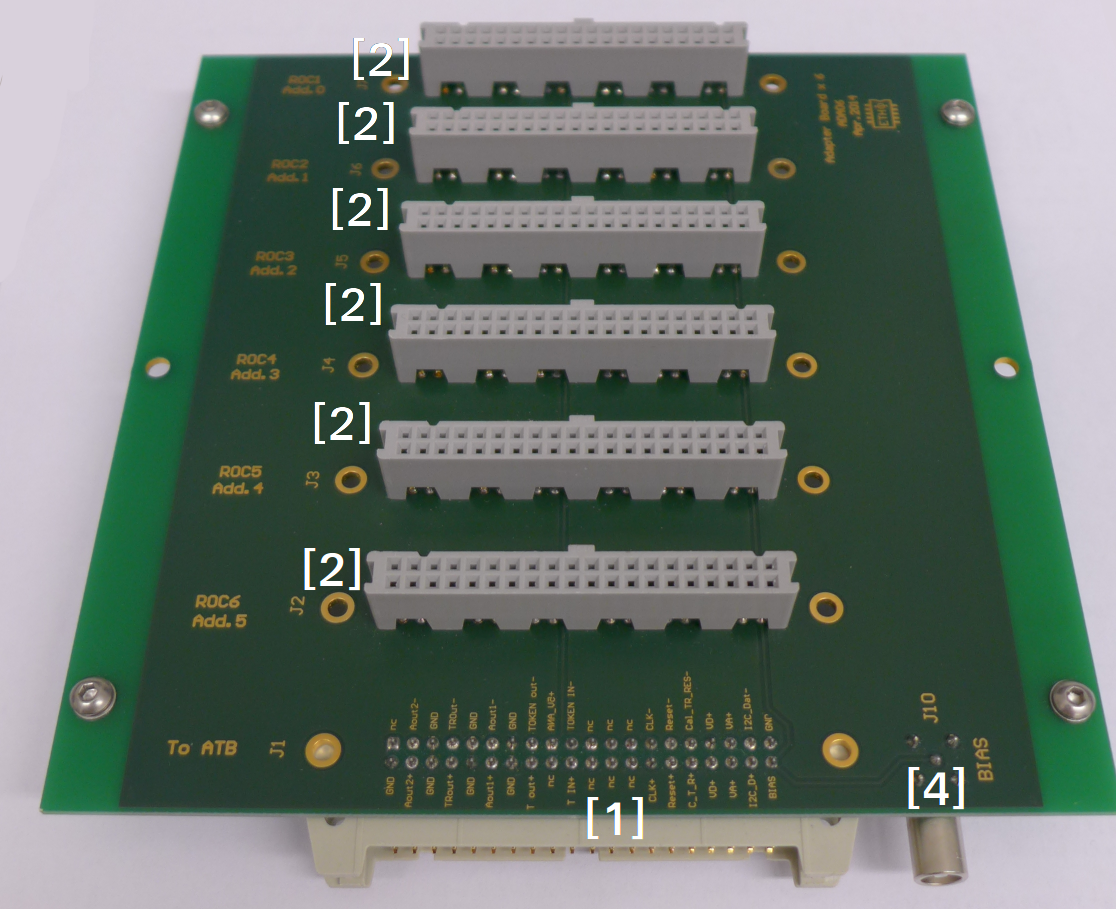
\includegraphics[width=0.52\textwidth]{setup/mb1}\label{p0}}
	\hfill
	\subbottom[Version 2]{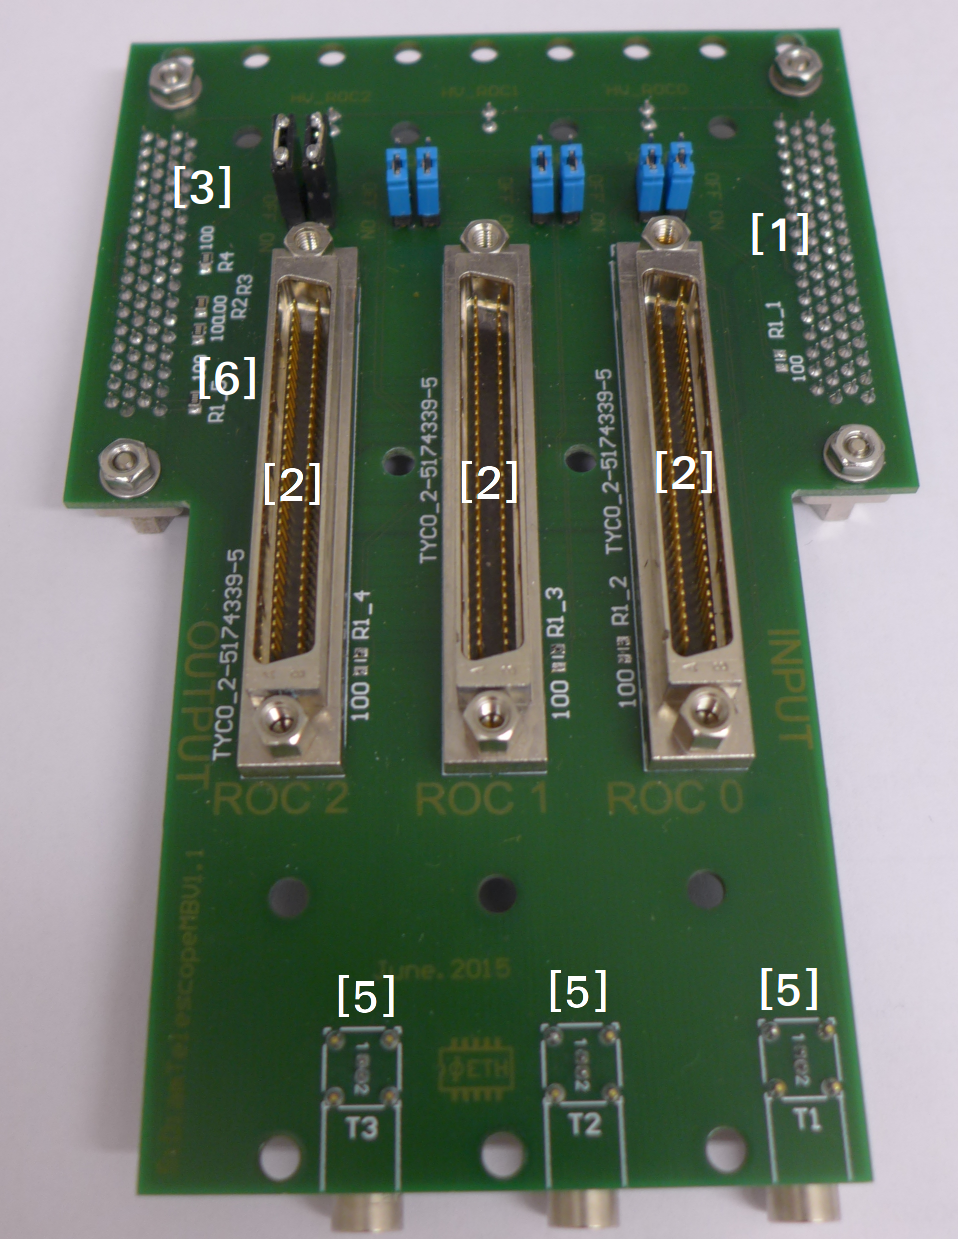
\includegraphics[width=0.42\textwidth]{setup/mb2}\label{p1}}
	\caption{The motherboards of the two telescopes}
	\label{pmb}
\end{figure}\no
The \ac{PCB} has a male connector [1] for a data transfer cable to communicate with a test board. In case of version 2 there is a second male [3] connector to which another telescope may be connected and that can only be used only as an output of the data stream. Next in line after the input come several daisy chained female connectors [2] to plug in the adapter planes. In order that the token can be sent through the whole chain, either the planes have to be plugged into [2] or a token jumper (\ar{pjumper}) has to be used. In addition version 1 has a LEMO connector [4] that allows to bias all of the connected sensors and version 2 has a differential LEMO outputs [5] for the fast-OR of every plane. All signals that pass through the telescope are properly terminated by resistors on the motherboard\footnote{In case of version 1 the resistors are underneath the board}. In case of version 2 there are boards with and without resistors and one should take care that only the last board in the chain is one with termination. Otherwise the signals might get too low to be measured.\\
The main differences of the two versions are stated in \ar{t1}.\\
The version 1 of the telescope was limited to a maximum of six static analogue planes. A main advantage of the other version is its flexibility to chain multiple three-plane telescopes together. Furthermore it easier and more convenient to place the token jumpers now. The Dimensions of the two telescopes are shown in \ar{pdim}.
\begin{table}[ht]
	\begin{tabularx}{\textwidth}{X|c|c}
		\noalign{\hrule height 2pt}
										& Version 1 			& Version 2 					\\\hline
		Connector type 					& ATA 40 pin 			& VHDCI 68 pin					\\			
		Number of planes per telescope 	& $6$ 					& $3$							\\
		Maximum number of Planes per read out chain		& $6$					& $3\times3$ \footnotemark[2] \\
		Fast-OR	output					& directly on the plane	& on the motherboard			\\
		Token jumper					& \ar{pjumper1}				& \ar{pjumper2}	\\
		\noalign{\hrule height 2pt}
	\end{tabularx}					
	\caption{Differences between the two motherboard versions}
	\label{t1}
\end{table}\no
\footnotetext[2]{Theoretically one could chain an infinite amount of telescopes. In reality the timing between the planes gets worse the longer the data has to travel, s.t. it not possible to read out more than three connected telescopes.}
\begin{figure}[ht]
	\centering
	\subbottom[Version 1: Self crafted token jumper by hard wiring the token line of a spare ATA connector. This jumper is then placed on the connector of the motherboard instead of a plane.]{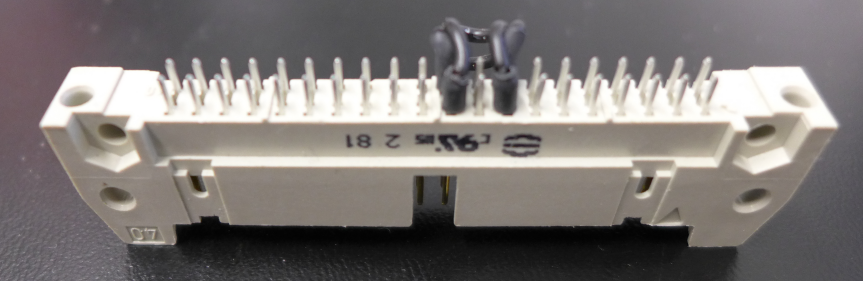
\includegraphics[width=0.47\textwidth]{TokenJumper}\label{pjumper1}}
	\hfill
	\subbottom[Version 2: The blue jumpers loop the token into the plane and the black jumpers make the token pass the plane. A blue jumper at the ``Out'' position will send the token into the next connected motherboard and a black one back to the \ac{DTB}]{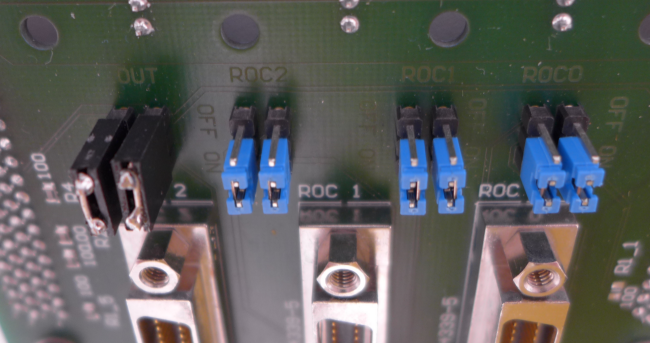
\includegraphics[width=0.47\textwidth]{setup/jumper2}\label{pjumper2}}
	\caption{The token jumpers for the two version of the telescope.}
	\label{pjumper}
\end{figure}\no
\begin{figure}[ht]
	\centering
	\subbottom[Version 1]{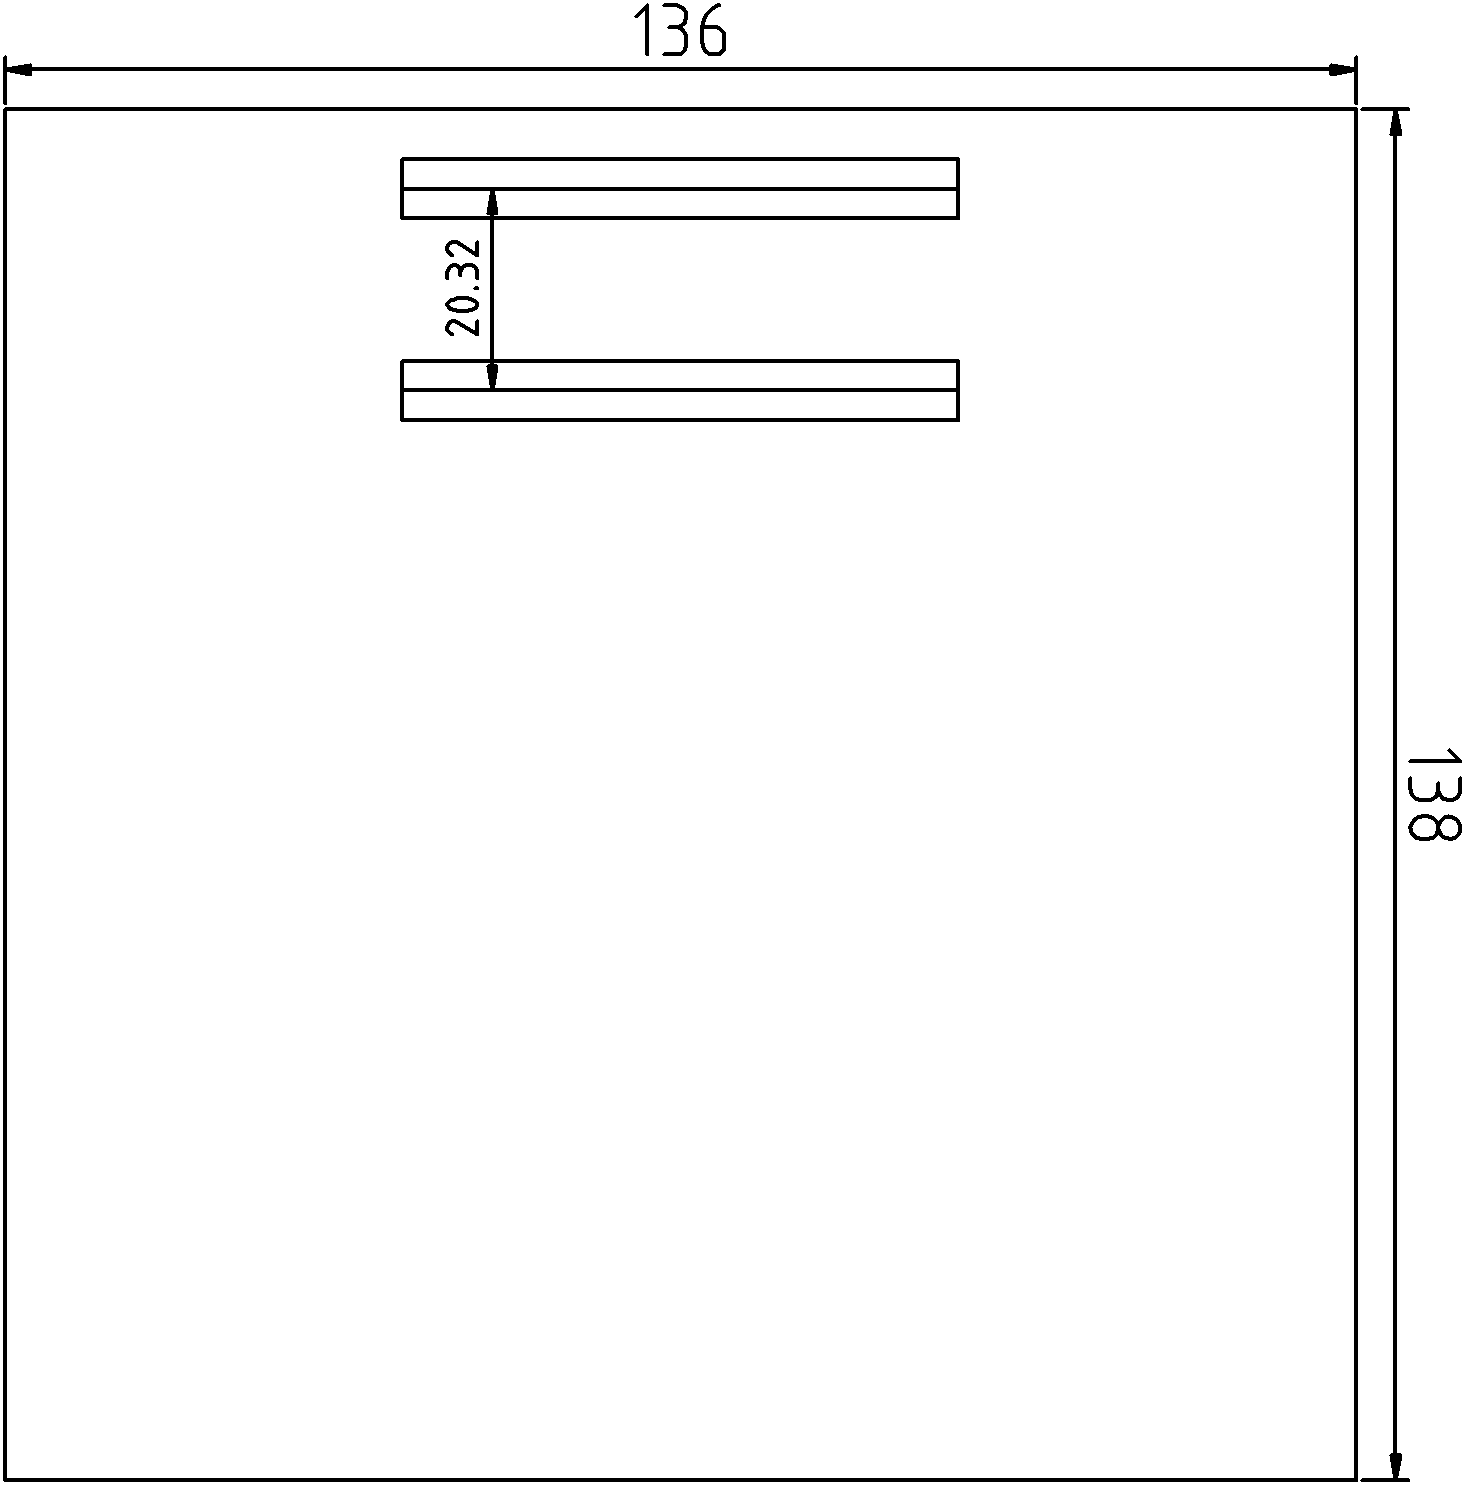
\includegraphics[width=0.47\textwidth]{dim1}\label{pdim1}}
	\hfill
	\subbottom[Version 2]{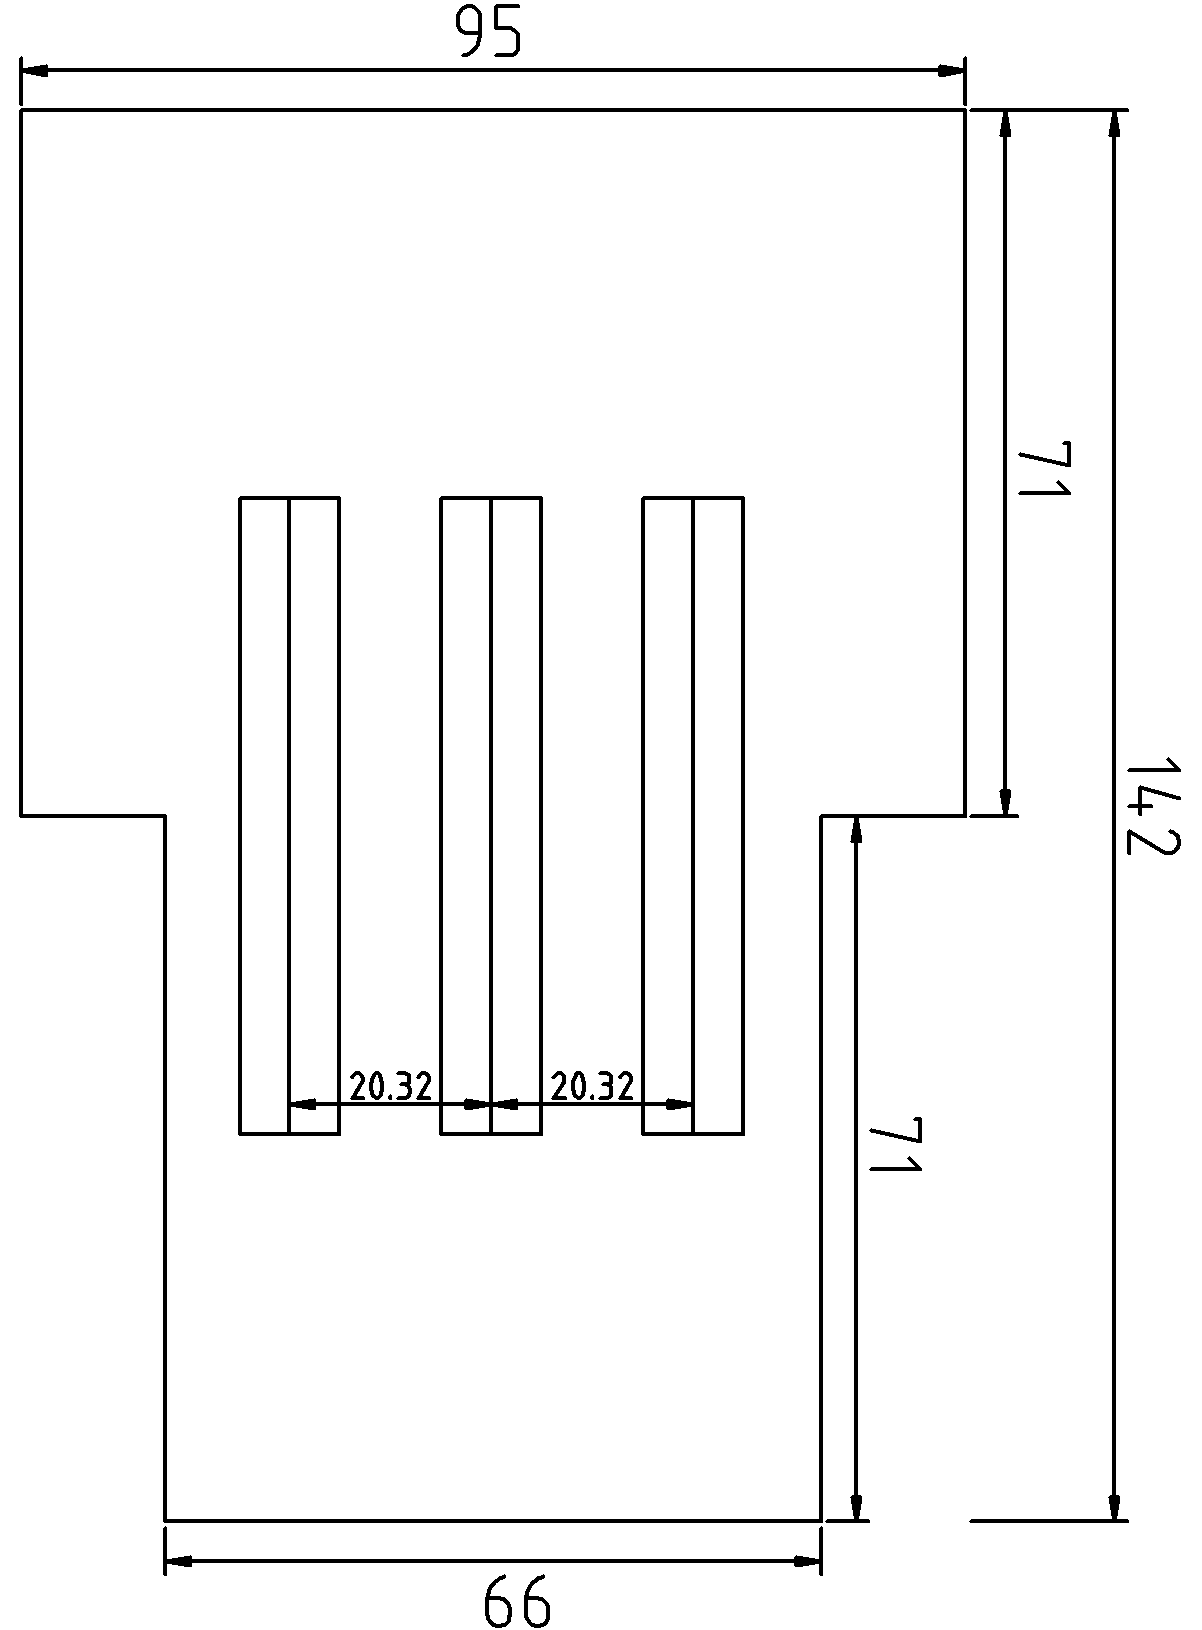
\includegraphics[width=0.47\textwidth]{dim2}\label{pdim2}}
	\caption{Dimensions of the two motherboards in millimetres.}
	\label{pdim}
\end{figure}\no
% ========================================================
\newpage
\subsection{Adapter Plane}\label{s211}
The adapter plane is the link between the telescope and a single \ac{CMS}-Pixel 
\begin{wrapfigure}{r}{5cm}
	\vspace*{-10pt}
	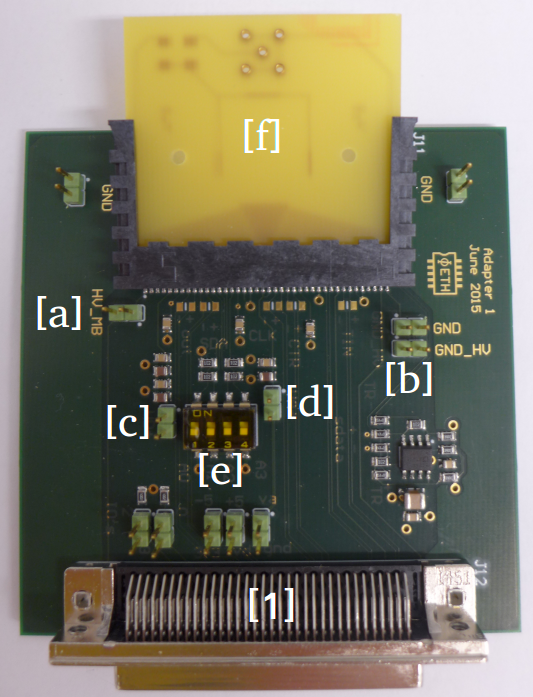
\includegraphics[width=5cm]{setup/digada}
	\caption{Digital adapter plane.}
	\label{p6}
	\vspace*{-5pt}
\end{wrapfigure} 
chip. The numbers in the following description refer to parts in \ar{p6} and \ar{padaana}. On the bottom end of the \ac{PCB} is a male connector [1] with which the plane can be plugged directly into the motherboard. The analogue planes of both telescope versions are very similar. Their differences are the already mentioned type of connector (\ar{t1}) and that there are two differential outputs for the fast-OR on the PCB of version 1 [2] (\ar{p4}) that were moved to the motherboard in version 2. Apart from that they both have an input for biasing the sensor [3], an amplifying circuit for the fast-OR [4], a small cable connector [5] to the \ac{ROC}\footnote[3]{This connector was already used for the \ac{PLT} and was kept since then.} and cable pins [6] to bias the \ac{ROC}. In version 2 there is an additional jumper [7] to allow biasing from either the adapter plane or via the connector to the motherboard. In both cases, the BIAS-GND pin of [8] has to be connected to the other outer pin of [8]. In order to bias the \ac{ROC} a cable [9] has to be connected from the BIAS- pin of [6] to the \ac{ROC} itself.\\
The adapter for the digital chips, which is shown in \ar{p6}, can only be used in combination with version 2 and differs a bit from the analogue one. The only way to bias the digital chips is via the test board and the SCSI connector, which means that there has to be a jumper at HV-MB [a] and GND-HV [b]. Likewise two jumpers have to connect the supply voltages VD [c] and VA [d] to the chip. Another very useful improvement is the dip switch box [e] in the middle of the plane, which allows to set any \ac{I2C} address between $0$ and $15$. Since the digital chips are put on special \ac{PCB}s [f], the adapter has a completely different mounting system, s.t. the chips can be easily plugged in and out, whereas the analogue \ac{ROC}s have to be screwed to the \ac{PCB}.
\begin{figure}[ht]
	\centering
	\subbottom[Version 1 without \ac{ROC}]{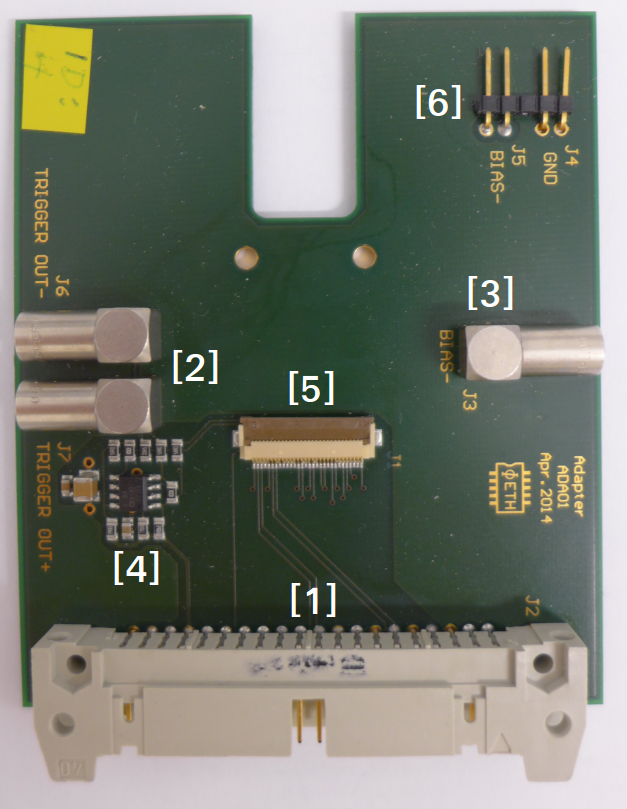
\includegraphics[width=0.47\textwidth]{setup/adaana1}\label{p4}}
	\hfill
	\subbottom[Version 2 with \ac{ROC} mounted underneath the black cover]{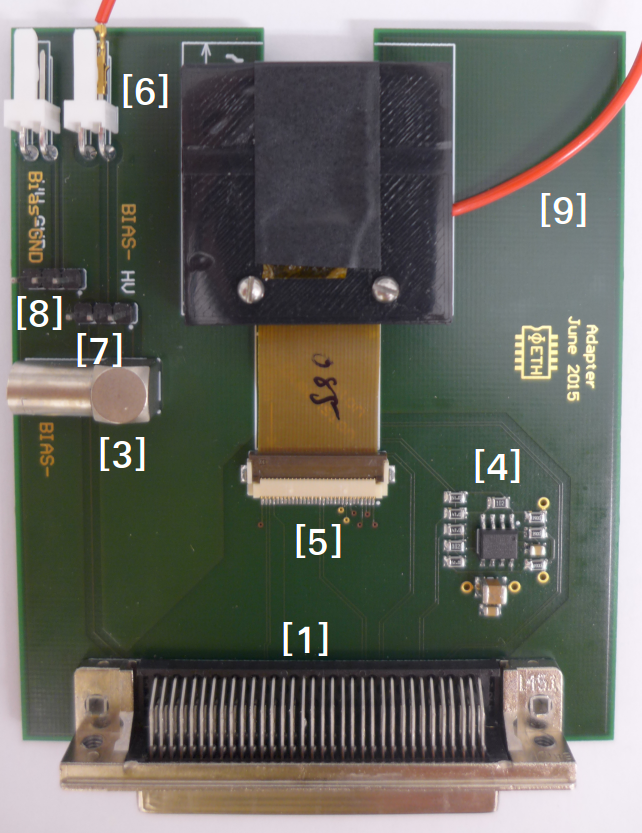
\includegraphics[width=0.47\textwidth]{setup/adaana2}\label{p5}}
	\caption{Analogue adapter planes of the two telescope versions.}
	\label{padaana}
\end{figure}\no
% ========================================================

\chapter{The Order of Matter - Set-up}
During the thesis a lot of various experiments were conducted that required different configurations of the telescope. In the next chapters these set-up are briefly summarised and sorted by complexity. 
% ========================================================
% SINGLE CHIP
% ========================================================
\section{Single \ac{ROC} Assembly}
The single \ac{ROC} set-up  is very important for basic functionality tests of a \ac{ROC} and for the general understanding of the chip. A real set-up a shown in \ar{psingleroc} and a general schematic drawn in \ar{psinglerocdraw}. It is possible to either connect an adapter plane directly to the \ac{ROC} or equip the telescope with a single plane and use jumpers at the vacant positions.
\begin{figure}[ht]
	\centering
	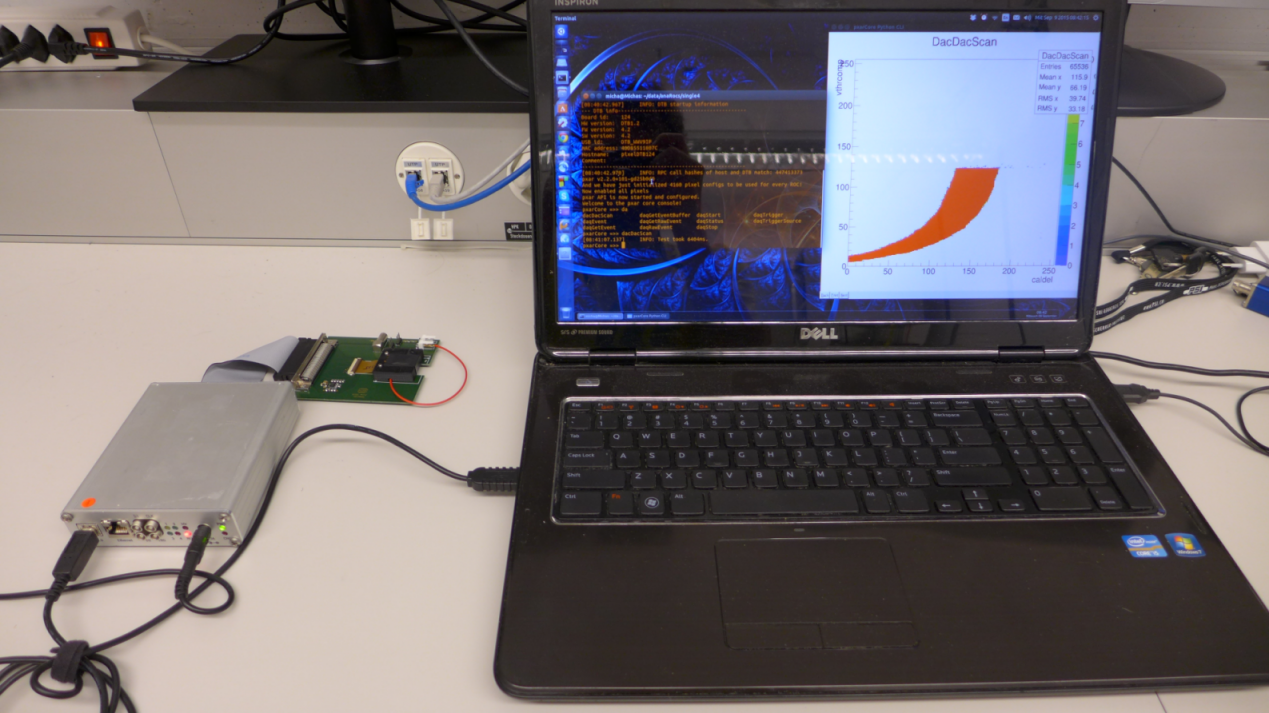
\includegraphics[width=0.95\textwidth]{setup/singlesetup}
	\caption{A single adapter plane operated with a \ac{DTB} connected to a laptop.}
	\label{psingleroc}
\end{figure}\no
\begin{figure}[ht]
	\centering
	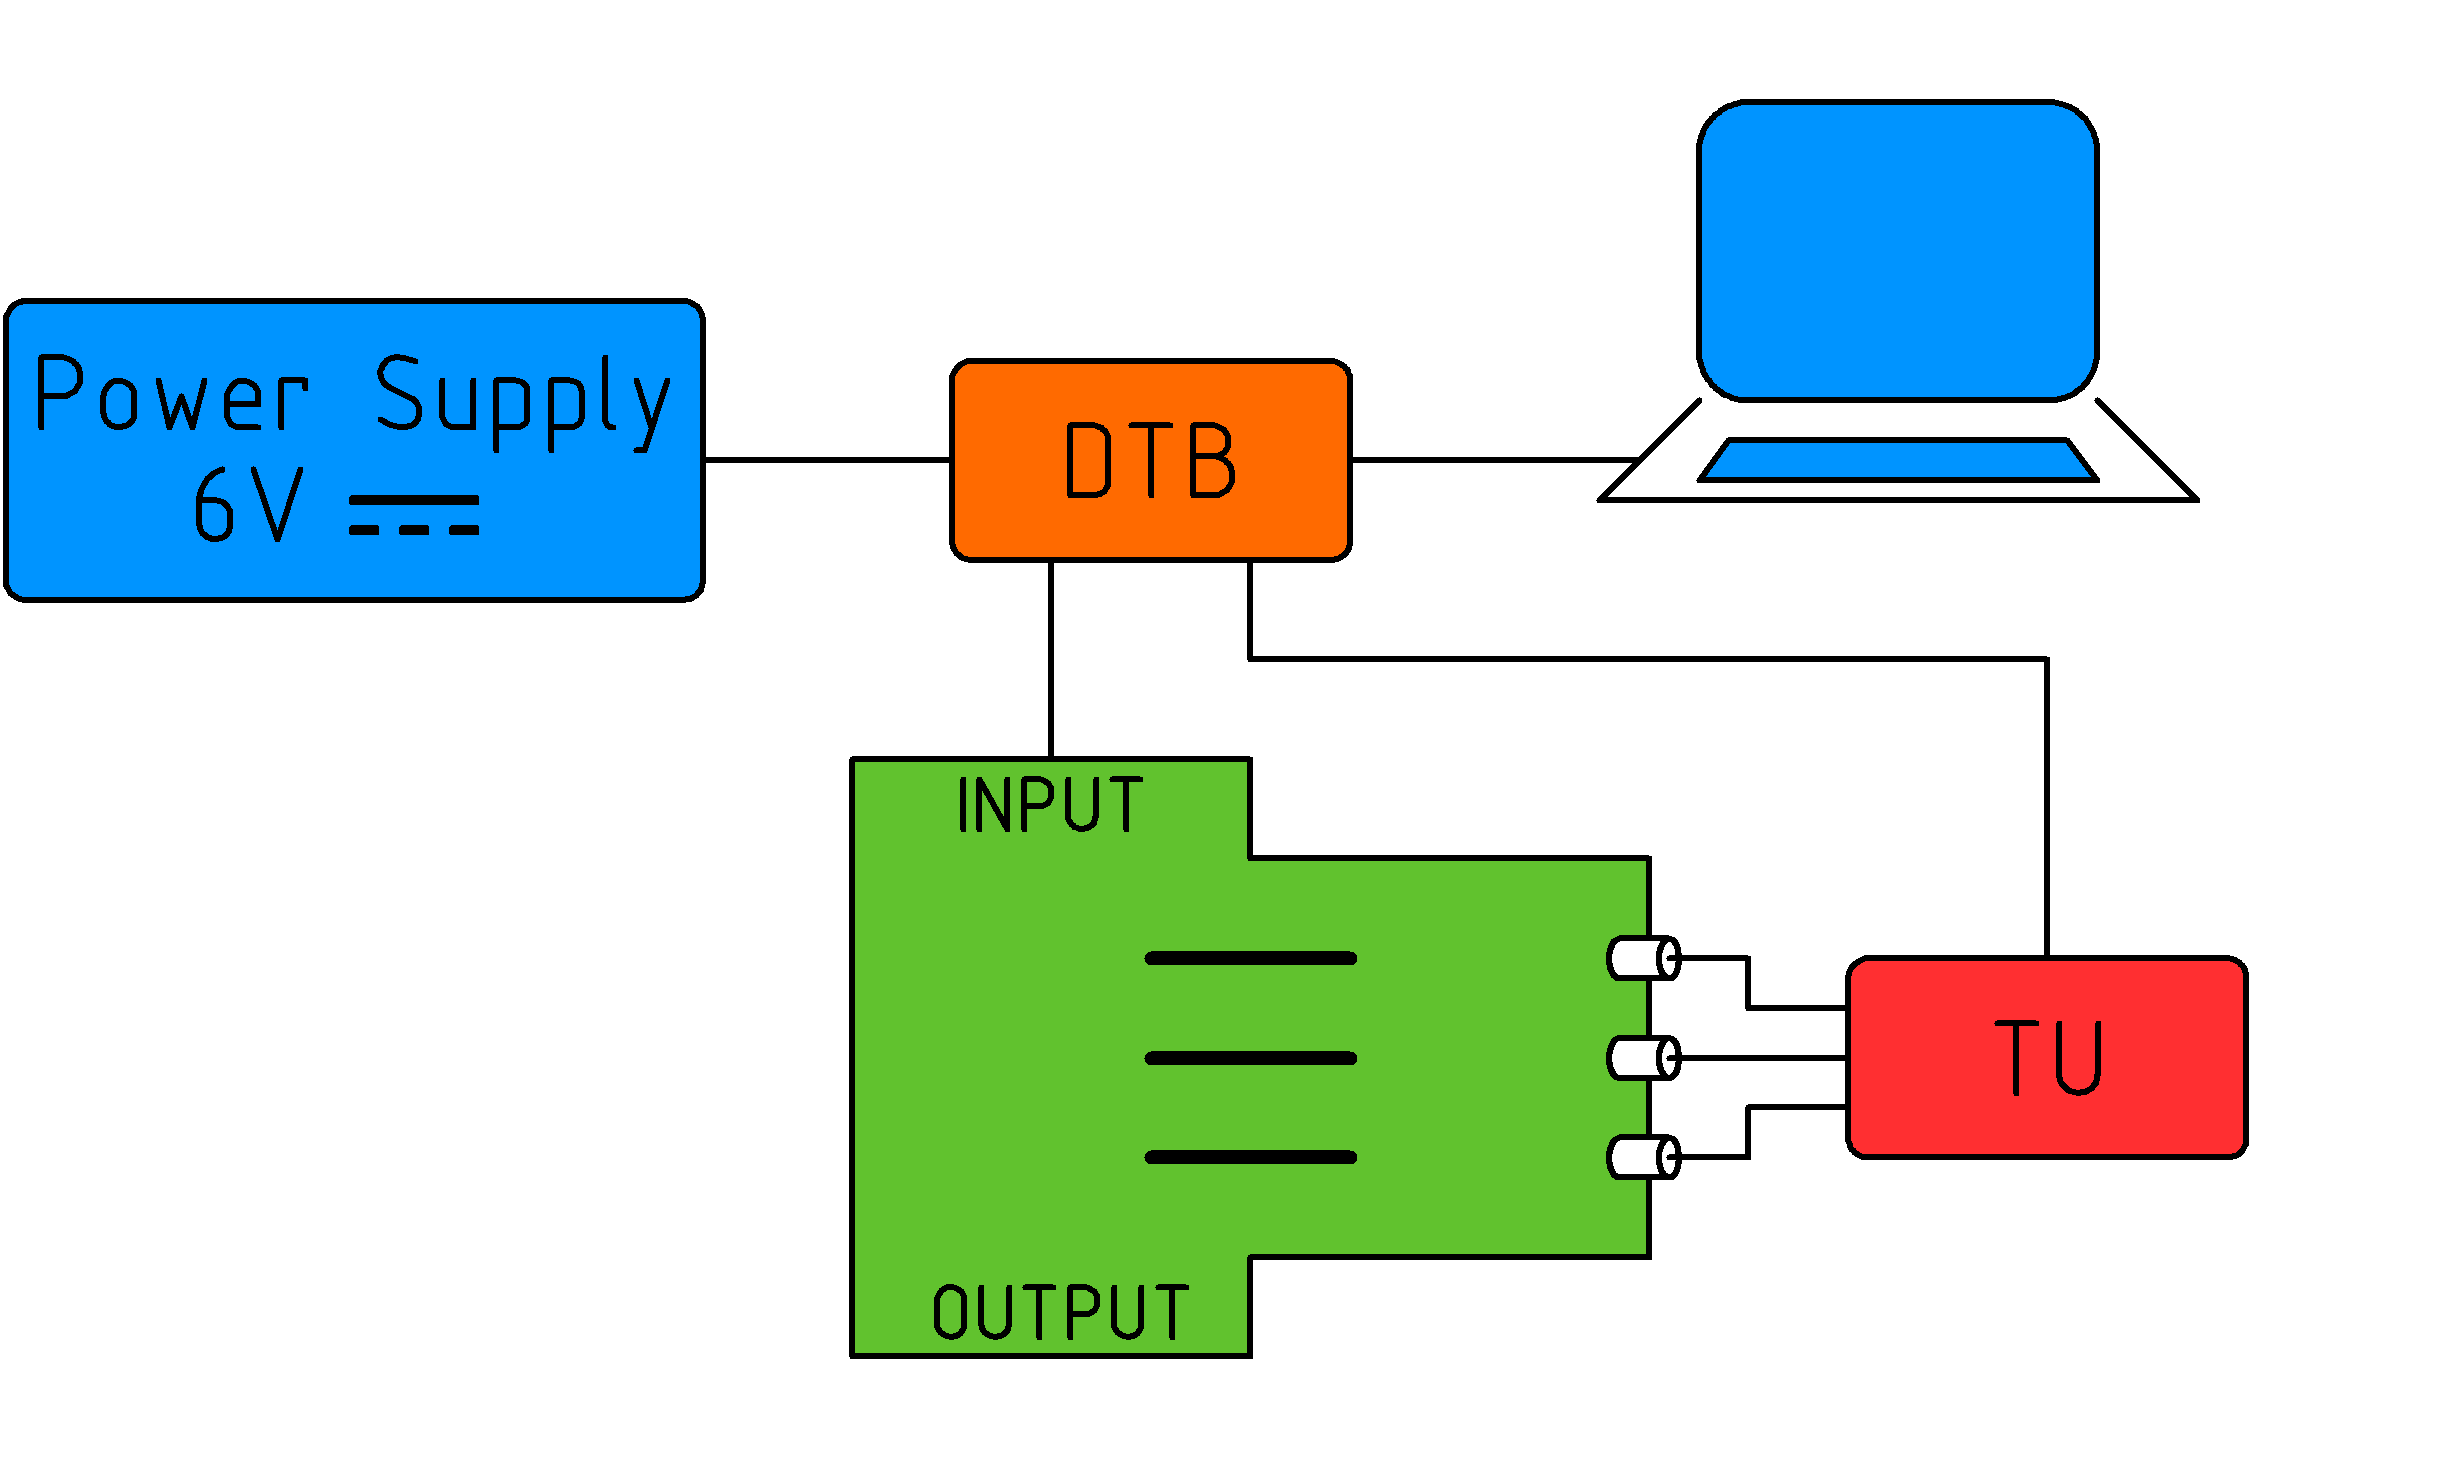
\includegraphics[width=0.6\textwidth]{singletel}
	\caption{Schematics of a single telescope set-up.}
	\label{psinglerocdraw}
\end{figure}\no
% ========================================================
\subsection{Simple Testing Set-up}
The most minimalistic set-up consists out of a single \ac{ROC}, the \ac{DTB} and a computer. It used for testing purposes using calibrate signals. Thus, it requires no external trigger source and the \ac{TU} in \ar{psinglerocdraw} is not required.
% ========================================================
\subsection{Source and External Trigger}
The above set-up can be extended with an external trigger. For almost every set-up\footnote{Exceptions are mentioned in \ar{sexp}} the fast-OR of the analogue \ac{ROC}s is used as trigger. Thus, the one plane set-up with external self trigger is only viable for the analogue chips.\\
In order to create particle hits, a radioactive \chemfig{Sr^{90}} source can be placed on top the \ac{ROC}. Thereby fast-ORs are generated which have to be sent back to the \ac{ROC} using the trigger logic in \ar{plogic1}. In this case with only one plane the coincidence unit is not required.
% ========================================================
\subsection{Trigger Logic}\label{striglog1}
The fast-ORs leaving the planes are differential signals, which is why their base line has a zero offset. Since we are using NIM the negative part of the differential signal is chosen and sent to a self made level shifter that shifts the baseline to zero. In order to transform the signal into a rectangular NIM pulse a discriminator is used next. This is done for the fast-ORs of all available planes in parallel. Every signal on its own is sent to a scaler to count the number of events for each plane. All signals together are sent to a coincidence unit, where the user can decide which effective trigger is used. It is possible, for example, to select only events with triggers in every plane by putting all fast-ORs in coincidence or to use only the trigger from a single plane and discard the rest. Afterwards the effective trigger rate is counted by a scaler. In a last step the effective trigger is converted into a \ac{TTL} signal by a \ac{TTL} converter. The signals is then distributed back to the planes via the \ac{DTB}.
\begin{figure}[ht]
	\centering
	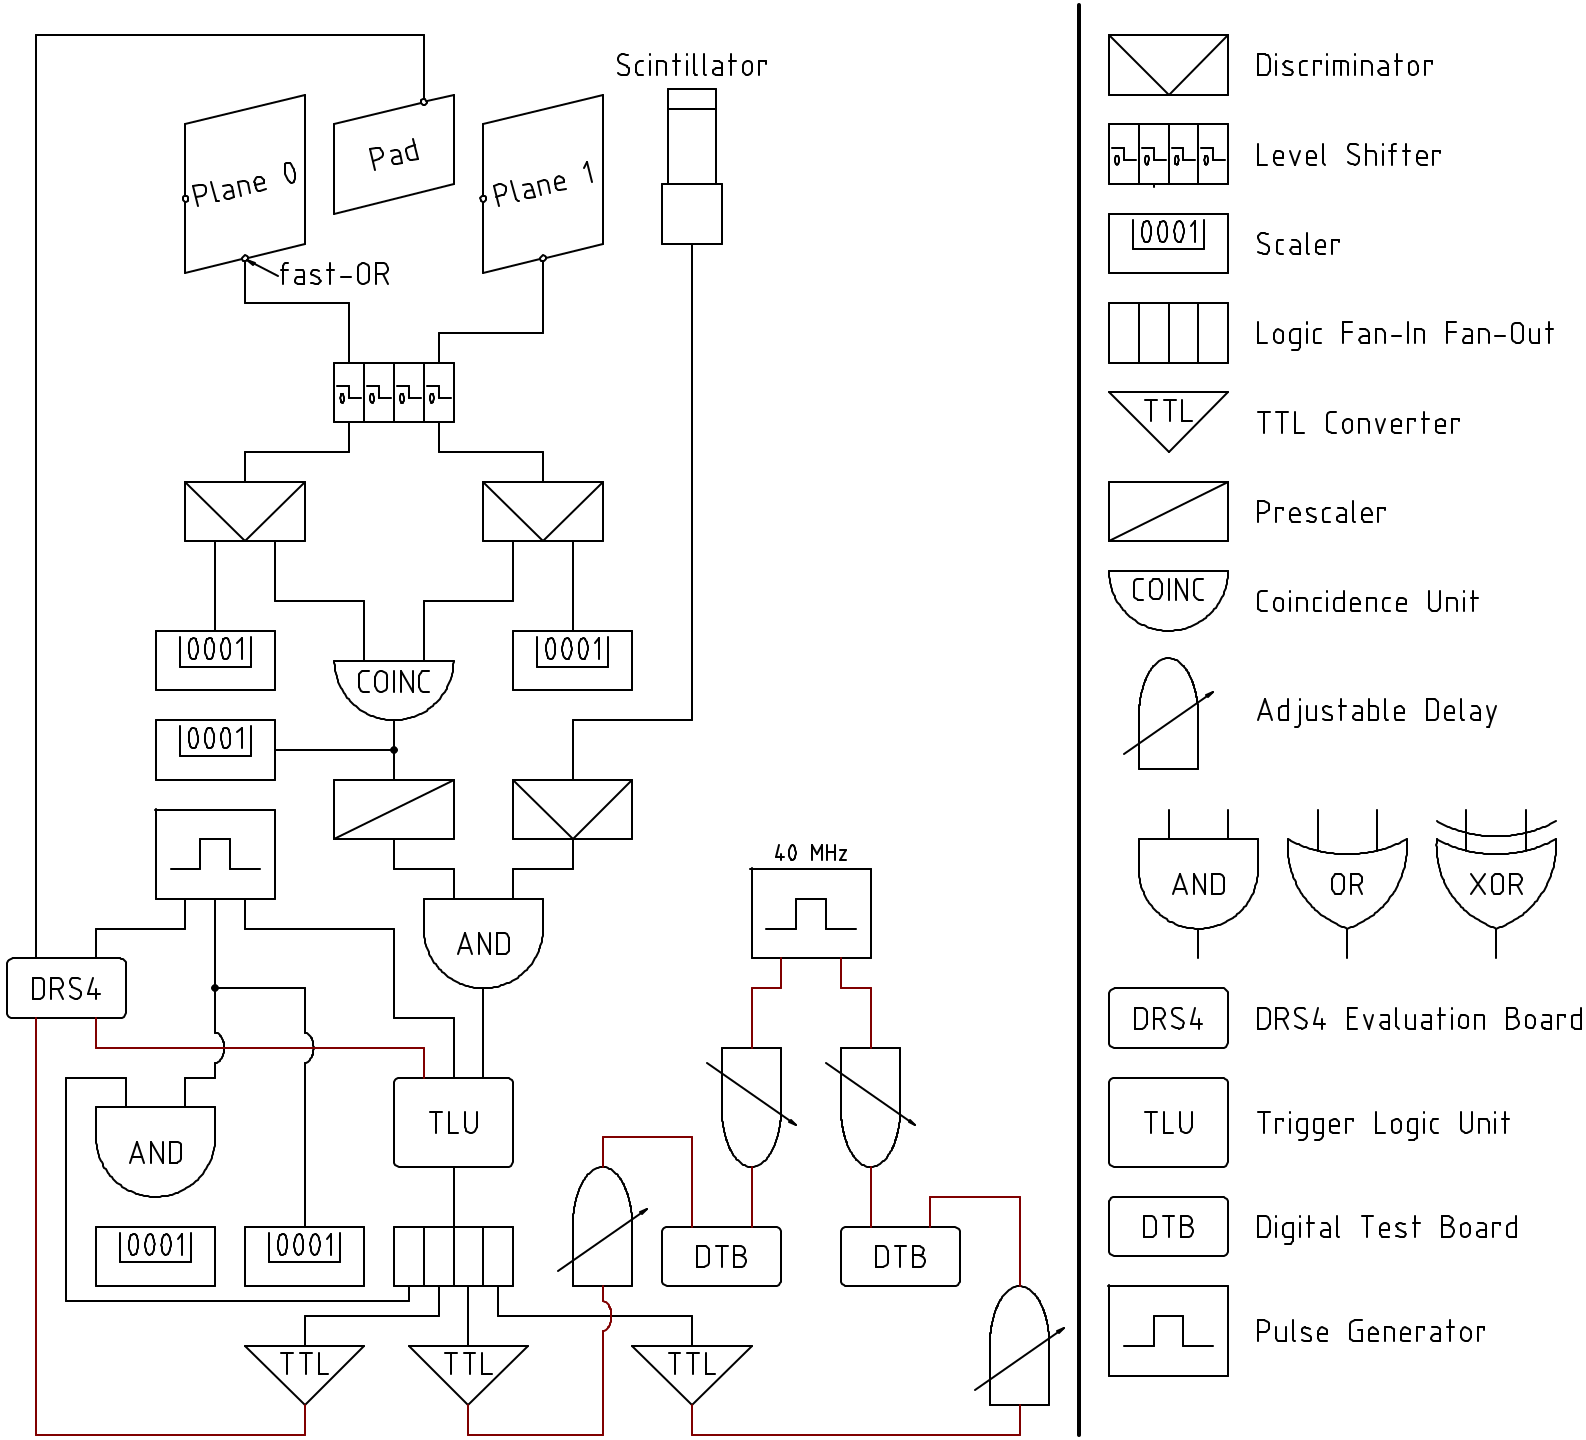
\includegraphics[width=0.6\textwidth]{triglog1}
	\caption{Simple trigger logic for a testing set-up. The number of planes may differ from the example, two was chosen for demonstration. To simplify matters, the connection from the \ac{DTB} to the planes is left out.}
	\label{plogic1}
\end{figure}\no
% ========================================================
% TELESCOPE
% ========================================================
\section{Single Telescope Set-up}
The single telescope set-up refers to a configuration with more than one plane in a single telescope controlled by a \ac{DTB}. Is very useful for the commissioning of the telescope using calibrate signals. Different numbers of planes can be tested. For external triggers the same logic as in \ar{striglog1} applies. However, the self trigger mode with a source is not possible for more than two planes because the beta electrons generally do not have enough energy to produce hits in more than two planes. A configuration with three planes is shown in \ar{p3plane}.
\begin{figure}[ht]
	\centering
	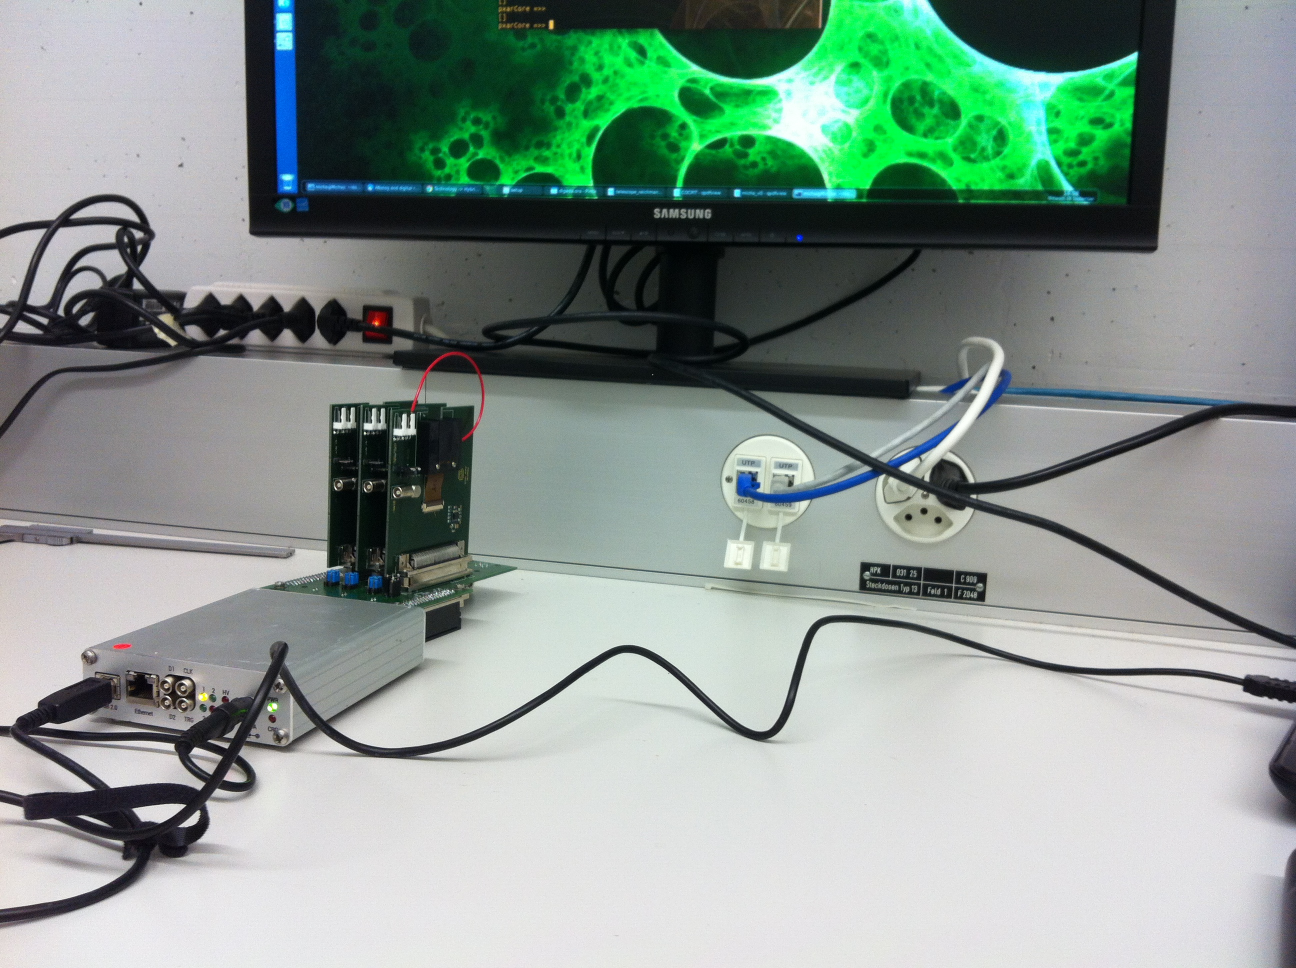
\includegraphics[width=0.95\textwidth]{3planetel}
	\caption{Telescope configured with three planes.}
	\label{p3plane}
\end{figure}\no
% ========================================================
% BEAM TEST
% ========================================================
\section{Beam Test Set-up}
In order to use the telescope to its full extent is has to placed inside of a particle beam of an accelerator. Being put there the telescope can be utilised on its own for debugging in self trigger mode with available fast-ORs for every single analogue plane. But the most important thing is to use it for its main purpose as auxiliary device for various \ac{DUT}s. A schematic visualisation of this set-up is shown in \ar{pfulldraw}. Every \ac{DUT} is placed inside a maximum number of six analogue planes that form a single telescope and are connected one \ac{DTB}. The trigger for all devices is the fast-OR of these analogue planes, which is handled by the trigger logic in \ar{plogic2}. During the beam tests for data taking usually two analogue were used in the front and the back adding up to a total number of four. The effective trigger almost always was a coincidence of the two inner planes, closest to the \ac{DUT}. The plastic scintillator at the end of the telescope is an optional device that used to get precise timing information about the particles; its signal is also fed to the trigger logic.\\
The examined types of \ac{DUT}s and their configuration within the telescope are named in the following:
\begin{itemize}
	\item one or two diamond pad detectors
	\item digital CMS pixel chips (silicon)
	\item digital CMS pixel chips with diamond as sensors
	\item pads combined with digital chips
	\item diamond and digital chips
\end{itemize}
The diamond pad detectors are made out of a single diamond sensor, whose signal is amplified and continuously read out by a DRS4 evaluation board. Digital and diamond pixel chips are placed inside the digital adapter planes and plugged into a motherboard which is controlled by a second \ac{DTB}. Two examples of these set-ups are shown out of different perspectives in \ar{sdut1} and \ar{sdut2}.
\begin{figure}[ht]
	\centering
	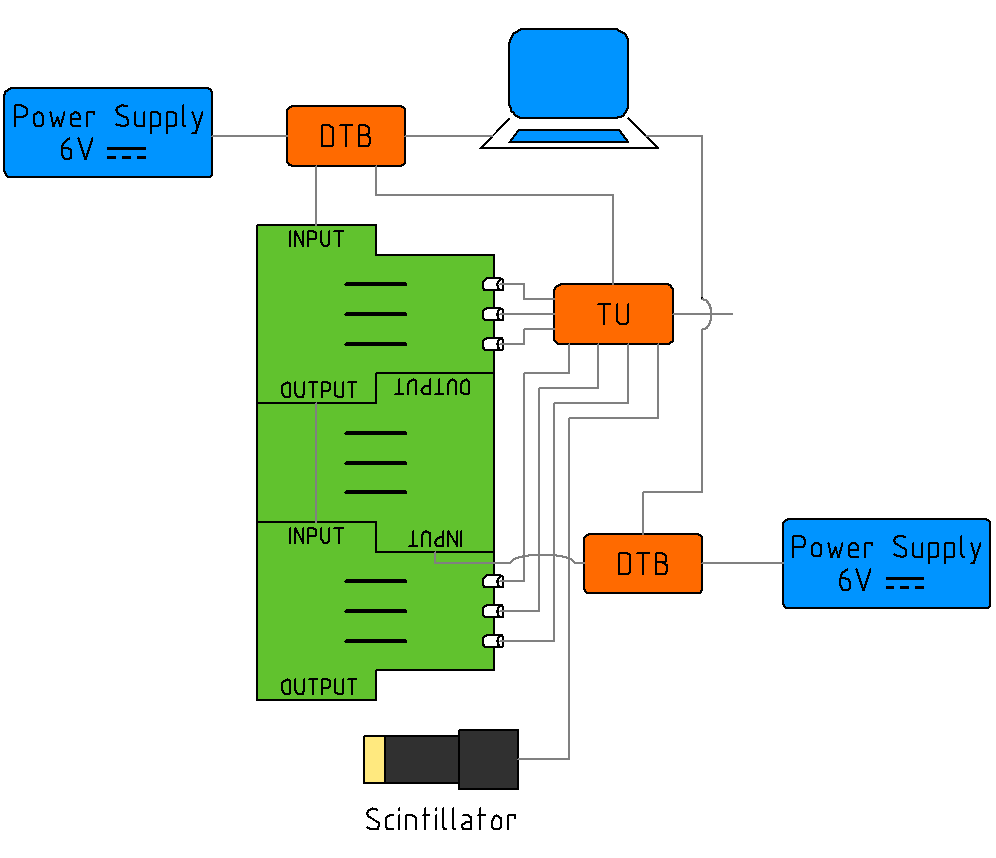
\includegraphics[width=0.9\textwidth]{felltel1}
	\caption{Schematics of a beam test set-up. The cables are drawn in grey to avoid confusion. To the open cable of the \ac{TU} may be connected to other devices like the DRS4 or a pulse generator. In this example a digital telescope is used as \ac{DUT} and placed between analogue planes. The two outer motherboards, which hold analogue planes are connected to each other and server a single telescope.}
	\label{pfulldraw}
\end{figure}\no
% ========================================================
\subsection{Trigger Logic}
The first part of the trigger logic for the beam test set-up is identical to the one described in \ar{striglog1}. Once the fast-ORs pass the coincidence unit there is a pre-scaling option to reduce the effective trigger rate. The effective trigger can then be brought into coincidence with a discriminated and delayable trigger signal from a scintillator. The scintillator delivers very precise timing information about the detected particles, which is used to determine the timing of a fast-OR trigger within one bunch crossing. The coincided signal is then sent together with two additional signals to a device called \ac{TLU}. The other two signal are the BUSY signal of the DRS4 that indicates a particle detection in the pad detector and a tunable clock from a pulse generator that is used as reference signal for the DRS4. If another \ac{DUT} than a pad is in use, the BUSY signal may be generated by the effective trigger itself.\\
The \ac{TLU} is a device especially built for beam test applications. Its main purpose is the exact distribution of trigger signals to the devices, synchronised with the data-taking software. Therefore it has a programmable a logic inside. For our purposes it makes an logic OR with the pulser and the effective trigger of the fast-ORs and the scintillator. Depending on the pulse length of the BUSY signal the \ac{TLU} will not send triggers once such a signal is received. In case of pad detectors this is required due to the dead time that arises when the DRS4 is processing an event.\\
The trigger that leaves the \ac{TLU} is then split by a fan-in fan-out and distributed to all the data-taking devices. \\
For the case of running with analogue and digital planes and respectively two \ac{DTB}s there is small extension. In order to synchronise the two \ac{DTB}s, a common clock that can be delayed for both of the boards, is sent to their external clock inputs. There is also the option to delay the trigger to each of the \ac{DTB}s. These four delays can then be used to optimise the trigger timing and the event alignment between the two boards. It therefore can improve the event yield.\\
In the future it is planned to use a \ac{TU} that unifies all the functions above, including the abilities of the \ac{TLU}, into a single device. It is currently under test at the Ohio State University. For this thesis everything was built using NIM modules in combination with the \ac{TLU}.
\begin{figure}[ht]
	\centering
	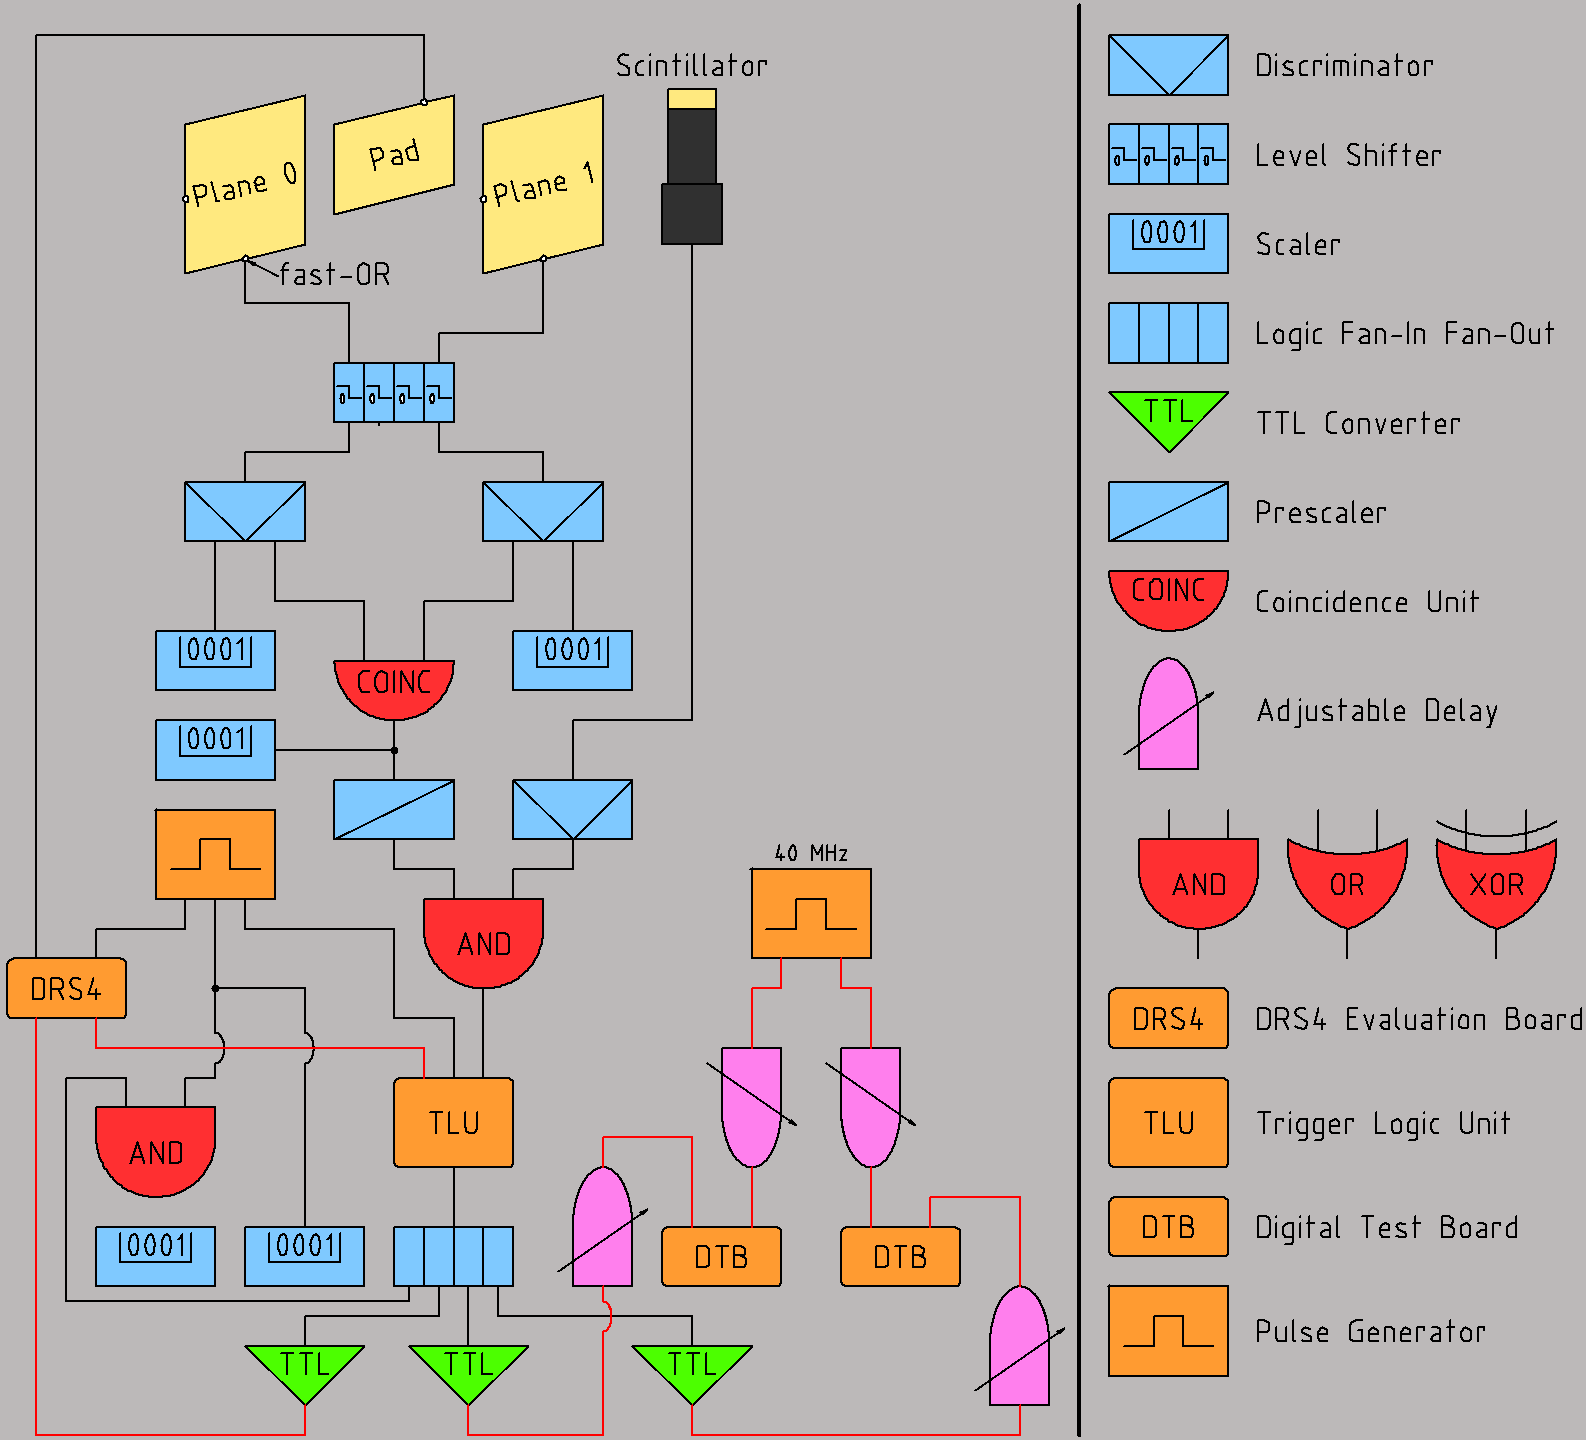
\includegraphics[width=0.95\textwidth]{triglog2}
	\caption{Full trigger logic. The pad may be exchanged with diamond pixels or other \ac{DUT}s. To simplify matters, the connection from the \ac{DTB} to the planes is left out. \ac{TTL} signal lines are drawn with red lines. The number of planes can also differ from this example.}
	\label{plogic2}
\end{figure}\no
\begin{figure}[ht]
	\centering
	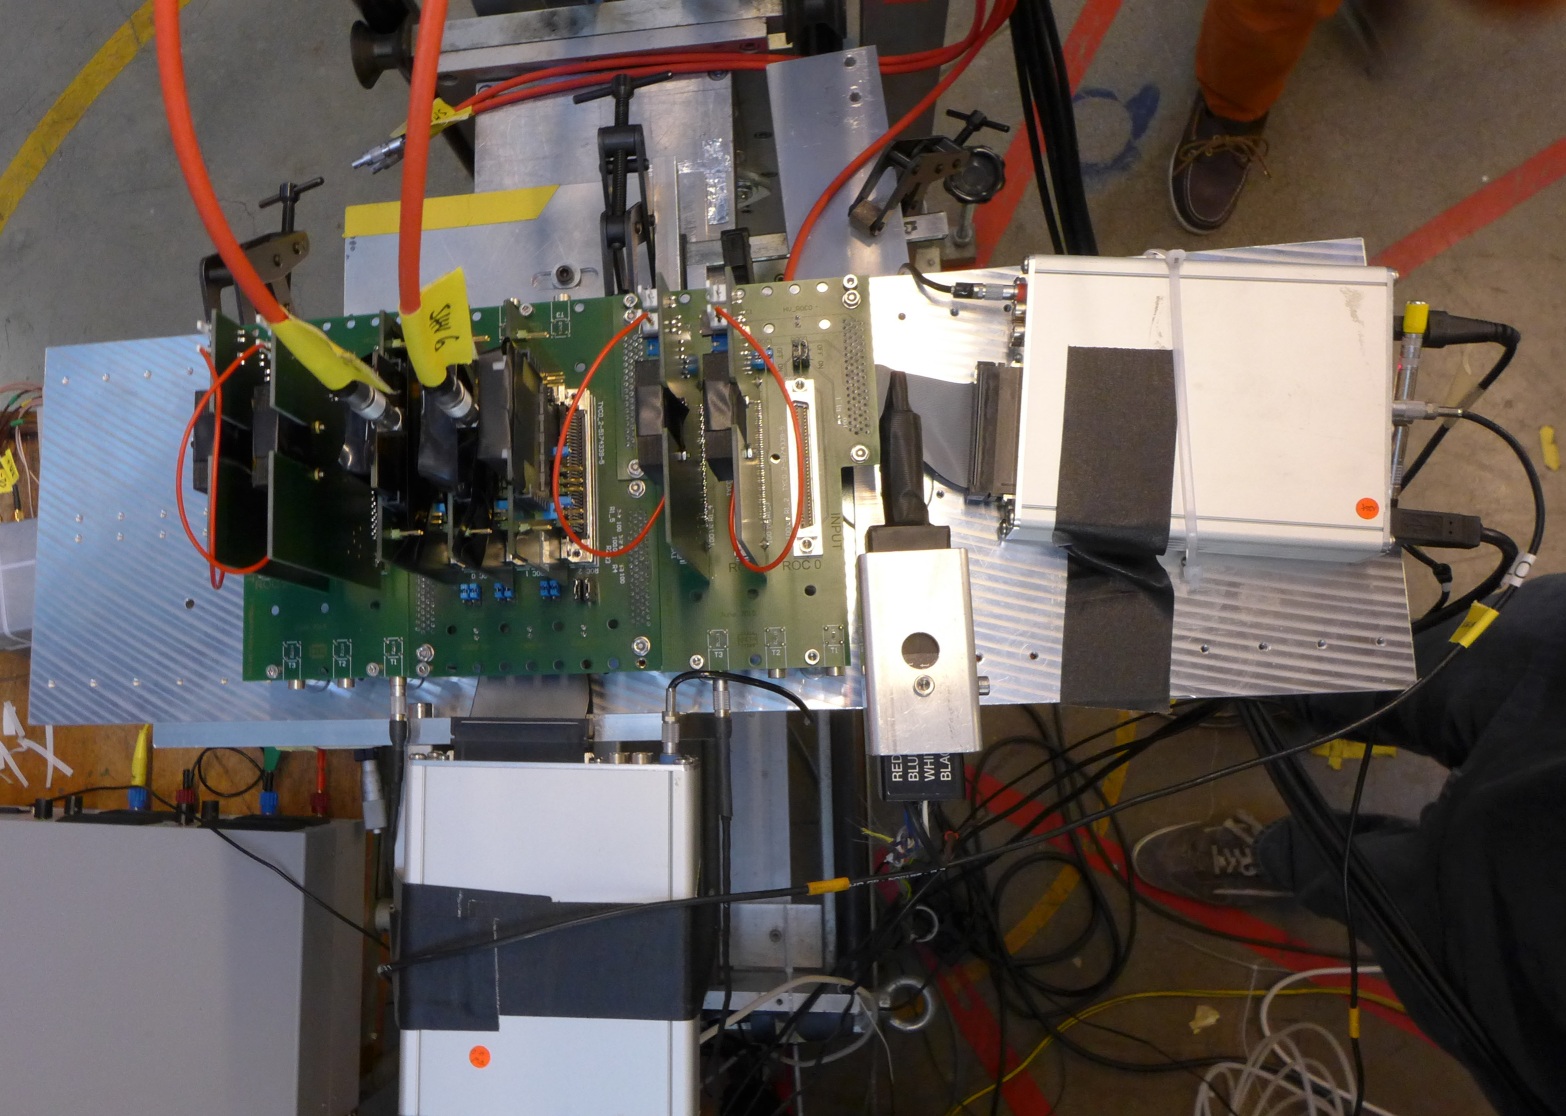
\includegraphics[width=0.95\textwidth]{setup/fullsetup}
	\caption{Top view of a beam test set-up at \ac{PSI}, the beam is coming from the left edge of the picture. The beam first hits two analogue planes on the first motherboard, afterwards two diamond pixel detectors and a digital silicon detectors on the next motherboard and then two analogue chips on a third motherboard. Last in line is a plastic scintillator. The four analogue chips are connected to the \ac{DTB} on the right side of the picture and the three digital chips to the test board in the front.}
	\label{sdut1}
\end{figure}\no
\begin{figure}[ht]
	\centering
	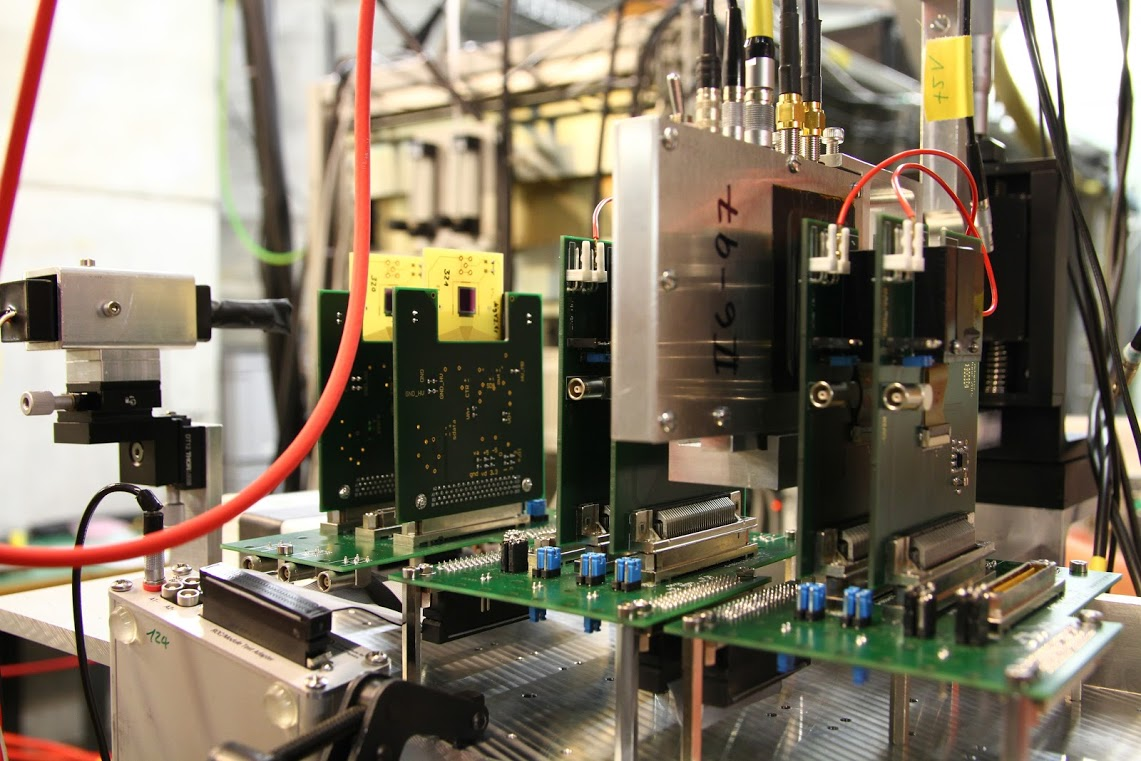
\includegraphics[width=0.95\textwidth]{setup/fullsetup1}
	\caption{Side view of beam test set-up at \ac{PSI}, the beam is coming from the right edge of the picture. The beam consecutively hits two analogue planes, a diamond pad detector and again two analogue planes. As mentioned before, the four analogue planes build one telescope. In the back are two digital silicon planes and a plastic scintillator, that were not used during this set-up.}
	\label{sdut2}
\end{figure}\no
% ========================================================

\chapter{The Doorway to the Information - Data Acquisition}

% ========================================================
% INTRO
% ========================================================
\section{Introduction}
In this chapter I am going to explain how the interfacing between a computer and the telescope is working, in which way the \ac{ROC} can be programmed and how the data is acquired and decoded by the software.\\
Basically all communication between the telescope and a computer is done via program called pXar, short for Pixel eXpert Analysis Readout, a pixel chip \ac{DAQ} and test suite. It was written by Simon Spannagel and Urs Langenegger to operate the digital \ac{ROC}. The program is completely composed in C++ and the main part, which talks to and programs the chips via the \ac{DTB}, is confined the so-called pXar-core and consists of a \ac{HAL} and an \ac{API}. Using the basic functions from the pXar-core library there are already a variety of tests that can be performed via the pXar-\ac{GUI}. For easier access and better flexibility Simon Spannagel also wrote a cython translation of the main pXar-core functions to make them accessible via python, which has the huge advantage to easily write own tests and use them via a python \ac{CLI}. To save the data of a single telescope one could also use pXar software, but since we are interested in the data combining with other instruments, e.g. pad detectors or second telescope, it is much more convenient to use the EUDAQ software.
% ========================================================
%TODO PUT that in the appendix
\section{Software}
The master branch of pXar and my own branch can be downloaded from git: 
\begin{itemize}
	\item \url{https://github.com/psi46/pxar}
	\item \url{https://github.com/michareichmann/pxar}
\end{itemize}
More information as well a detailed installation instruction can be found at the \ac{CMS} twiki: 
\begin{itemize}
	\item \url{https://twiki.cern.ch/twiki/bin/viewauth/CMS/Pxar} $rightarrow$ branch eth-2.0
\end{itemize}
The version of EUDAQ we were using can be found here: 
\begin{itemize}
	\item \url{https://github.com/veloxid/eudaq-drs4}. 
\end{itemize}
% ========================================================
% 1
% ========================================================
\section{pXar Core}

\includegraphics[width=4cm]{pxar_logo}
includes more than the main functions of the pXar-core I am going to present, but these are the components everything else is built on and I was using most of the time. An overview of the full software architecture is shown in \ar{p13}, the core consists of \ac{HAL} and \ac{API}.\\
The NIOS II soft core \ac{CPU} is a synthetic \ac{CPU} that is embedded in the \ac{FPGA} of the \ac{DTB}. It runs at $50\,$MHz and is used to perform very simple commands like starting the pattern generator. It's main purpose is the control of the \ac{DTB} functionality. Since the correct commands are automatically picked by the \ac{API} of the pXar-core, it is not further investigated. For further information look at \cite{spannagel}.
\begin{figure}[ht]
	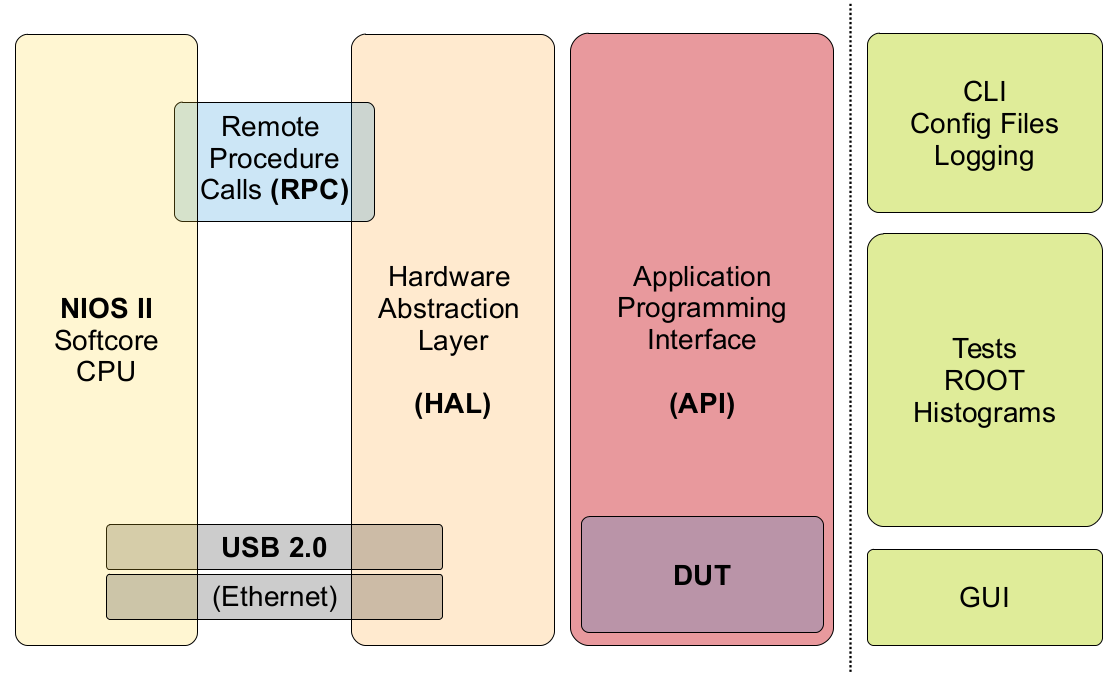
\includegraphics[width=0.95\textwidth]{pxar_scheme}
	\caption{software architecture of pXar \cite{spannagel}}
	\label{p13}
\end{figure}
% ========================================================
\subsection{\ac{HAL}}
The \ac{HAL} of the pXar-core is responsible for the direct communication with the \ac{DTB}. This is the part that has access to the RPC and USB. It supervises the data readout using pipes, which is a buffered readout of the data from the test board.\\
\hspace*{\dimexpr0.5\linewidth-5cm}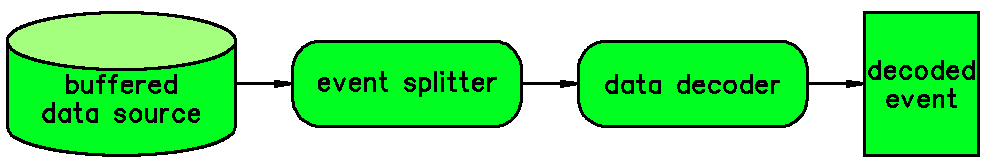
\includegraphics[width=10cm]{hal_buf}\\
The pipes can be set up for different purposes, either to deliver fully decoded events or ``raw'' events that are only split by the emulated \ac{TBM} header and trailer or complete raw data from the \ac{DTB}. The second option is very useful to debug the system, because it makes it easier to decide why something is not working. The last option may be useful for debugging too, but is mainly used for saving the raw data to a binary file.\\
Most of the basic functions with a short explanation are listed in \ar{t5}. They are loosely divided in categories i.e. basically all them can be used while the \ac{DTB} and pXar are running. So, having them in the group ``Device Initialisation'', means that they are used while initialising the board even though the may be reused afterwards.  \\
\begin{table}[ht]
	\begin{tabularx}{\textwidth}{l|X}
		\noalign{\hrule height 2pt}
		\multicolumn{2}{c}{\textbf{Device Initialisation}}							\\\noalign{\hrule height 2pt}
		\multicolumn{1}{c}{\textbf{command}}	& 	\multicolumn{1}{c}{\textbf{purpose}}	\\\hline
		initTestboard		& initialises the \ac{DTB} with its device specific \textit{signal delay} settings		\\
		setTestboardPower	& sets the \textit{analogue} and \textit{digital voltage} and \textit{current limits}		\\
		setTestboardDelays	& sets \textit{signal delay} settings		\\
		flashTestboard		& flashes a given \textit{firmware file} to the \ac{FPGA}		\\
		initROC				& initialises a \ac{ROC}s of a given \textit{type} with \textit{\ac{I2C} address} with a \textit{vector of \ac{DAC}s} 		\\
		SetupPatternGenerator	& sets the \ac{PG} to a given sequence		\\
		SetClockSource		& set clock source to internal or external		\\
		\noalign{\hrule height 2pt}
	\end{tabularx}
	\caption{base commands of \ac{HAL}}
	\label{t5}
\end{table}

\begin{table}[ht]
	\begin{tabularx}{\textwidth}{l|X}
		\noalign{\hrule height 2pt}
		\multicolumn{2}{c}{\textbf{\ac{DTB} Commands}}							\\\noalign{\hrule height 2pt}
		\multicolumn{1}{c}{\textbf{command}}	& 	\multicolumn{1}{c}{\textbf{purpose}}	\\\hline
		getTBia			& reads analogue current from \ac{DTB}		\\
		getTBva			& reads analogue voltage		\\
		getTBid			& reads digital current		\\
		getTBvd			& reads digital voltage		\\
		set*			& sets the limit of *$=$TBia, TBva, TBid, TBvd		\\
		SignalProbe*	& lays one of the internal \textit{signals} to the output *$=$D1, D2, A1, A2 		\\
		HVoff			& disables the \ac{HV} from the \ac{DTB} to the \ac{ROC}		\\
		HVon			& enables \ac{HV}		\\
		Pon 			& turns on power of the \ac{DTB}		\\
		Poff			& turns off power		\\
		rocSetDAC		& sets the \textit{\ac{DAC}} with \textit{\ac{I2C}} to a given \textit{value} 		\\
		\noalign{\hrule height 2pt}
	\end{tabularx}
	\caption{base commands of \ac{HAL}}
	\label{t6}
\end{table}

\begin{table}[ht]
	\begin{tabularx}{\textwidth}{l|X}
		\noalign{\hrule height 2pt}
		\multicolumn{2}{c}{\textbf{\ac{DAQ} Functions}}							\\\noalign{\hrule height 2pt}
		\multicolumn{1}{c}{\textbf{command}}	& 	\multicolumn{1}{c}{\textbf{purpose}}	\\\hline
		daqStart		& starts a new \ac{DAQ} session		\\
		daqTriggerSource& sets the trigger source (e.g. extern, pg)		\\
		daqTrigger		& sends out a given \textit{number} of \ac{PG} sequences with \textit{period} 		\\
		daqStop			& stop the current \ac{DAQ} session		\\
		daqEvent		& reads out a decoded event from the buffer if \ac{DAQ} is activated		\\
		daqRawEvent		& reads out a raw event		\\
		daqAllRawEvents	& reads out all events in the buffer		\\
		daqClear		& clears the buffer		\\
		\noalign{\hrule height 2pt}
	\end{tabularx}
	\caption{base commands of \ac{HAL}}
	\label{t7}
\end{table}

\begin{table}[ht]
	\begin{tabularx}{\textwidth}{l|X}
		\noalign{\hrule height 2pt}
		\multicolumn{2}{c}{\textbf{\ac{ROC} Functions}}						\\\noalign{\hrule height 2pt}
		\multicolumn{1}{c}{\textbf{command}}	& 	\multicolumn{1}{c}{\textbf{purpose}}	\\\hline
		SetupI2CValues		& sets the available \textit{\ac{I2C}} addresses		\\
		SetupTrimValues		& sets the trim bits from a given \textit{vector} for a \ac{ROC} with \textit{\ac{I2C}}		\\
		RocSetMask			& masks all pixels given in a \textit{vector}  for a \ac{ROC} with \textit{\ac{I2C}}		\\
		PixelSetCalibrate	& enables the calibrate signal for a pixel with \textit{col}, \textit{row} and \textit{\ac{I2C}}		\\
		RocClearCalibrate	& disables the calibrates for a \ac{ROC} with \textit{\ac{I2C}}		\\
		\noalign{\hrule height 2pt}
	\end{tabularx}
	\caption{base commands of \ac{HAL}}
	\label{t8}
\end{table}
% ========================================================
\subsection{\ac{API}}
The \ac{API} is the interface to the user, this is where all the commands are directed to. It is set-up in a way that it already does a lot of data pre-processing, i.e. it does assertions, range- and sanity checks for most the input parameters and commands. Thereby it is more user-friendly and a lot misusage can be avoided. To do that, it picks up the commands and functions from \ac{HAL}, the most important ones are listed in \ar{t9}\\
Included inside the \ac{API} is the self-contained \ac{DUT} class, which is responsible for the set-up of all the devices. It also saves the detector settings and makes them available all the time. The \ac{DUT} itself is initialised by the \ac{API} function initDUT($\hdots$), it is compatible with single \ac{ROC}s of both types, \ac{TBM}s or full modules. Mandatory information to start it for a single \ac{ROC} is a list of pairs of \ac{DAC}s and their values and trim bit values for all $4160$ pixels.
\begin{table}[ht]
	\begin{tabularx}{\textwidth}{l|X}
		\noalign{\hrule height 2pt}
		\multicolumn{2}{c}{\textbf{main \ac{API} functions}}						\\\noalign{\hrule height 2pt}
		\multicolumn{1}{c}{\textbf{command}}	& 	\multicolumn{1}{c}{\textbf{purpose}}	\\\hline
		initTestboard		& checks weather power setting, \ac{DTB} delays and \ac{PG} settings are viable and then start \ac{HAL} command			\\
		setDAC				& verifies that the \ac{DAC} setting are sane and then starts rocSetDAC		\\
		setExternalClock	& checks weather there is an external clock present and uses SetClockSource accordingly		\\
		daqStart			& uses daqClear, resets the mask, calibrate enable and trim settings, starts \ac{DAQ} with daqStart	from \ac{HAL}			\\
		daqStatus			& returns the status of the \ac{DAQ} 			\\
		getNEnabledPixels	& returns the number of pixels enabled for calibrates			\\
		getNMaskedPixels	& returns the number of masked pixels			\\
		getRocType			& return the \ac{ROC}-type 			\\
		testPixel			& enables the pixel with \textit{column}, \textit{row} and \textit{\ac{I2C}} and check if the pixel exists for the given \ac{ROC}			\\
		maskPixel			& masks the pixel with \textit{column}, \textit{row} and \textit{\ac{I2C}} and check if the pixel exists for the given \ac{ROC}	 			\\
		\noalign{\hrule height 2pt}
	\end{tabularx}
	\caption{base commands of \ac{API}}
	\label{t9}
\end{table}
% ========================================================
% 2
% ========================================================
\section{Decoder}
In this section I am going to describe the basic steps how the raw data from the analogue chip is decoded with pXar, which is very useful while debugging possible decoding issues and to guarantee a stable readout at all. Since pXar was made for reading out the digital chip whose \ac{ADC} is included in the \ac{ROC}, the decoding of this chip is working well and did not require any further investigation.\\
After passing the \ac{ADC} of the \ac{DTB} and the soft \ac{TBM} the raw data looks like this:
\begin{center}
\terminal{[36600, 4027, 29, 3980, 4083, 39, 90, 141, 16427]}                                                    
\end{center}
Each raw data blob consists of $16\,$bit data words of which only the last $12\,$bits contain the data, which also correspond to the output range of \ac{DTB}'s \ac{ADC}. The first four bits are used to mark the beginning and the end of a data blob. So the first step is to reduce the first four bits with a bitwise AND which sets the first four bits to zero:
\begin{equation}
	\z{dataword} = \z{dataword}\ \&\ 0\z{x}0\z{fff}\footnote{the prefix ``0x'' heralds a hexdecimal number} \equiv \z{dataword}\ \&\ \left( 2^{12} - 1\right)
\end{equation}
\begin{center}
\terminal{[3832, 4027, 29, 3980, 4083, 39, 90, 141, 43]}                                                    
\end{center}
Because the \ac{ADC} only gives out positive integers, the positive $12\,$bit range is split into two parts where the first $2^{11}$ values correspond to positive values and the second half to the negative ones. So to convert them to their negative equivalent one has to subtract the integers larger than $2^{11}$ by $2^{12}$:
\begin{equation}
	\begin{split}
		&\z{if } \z{dataword}>0\z{x}0800:\\
		&\ \ \ \ \z{dataword} = \z{dataword}\ - 0\z{x}1000 \equiv \z{dataword} - 4096
	\end{split}
\end{equation}
\begin{center}
\terminal{[-264, -69, 29, -116, -13, 39, 90, 141, 43]}                                                    
\end{center}
Now we got the values that correspond to the analogue signal. Due to various effects (e.g. different supply voltages and \ac{DAC} settings) the absolute values of the levels may vary in the whole range of the \ac{ADC}, but their spacing to one another and their offset is determined by the \ac{UB} and \ac{B} level of the \ac{ROC} header. As already mentioned in \ar{s221}, the data stream always starts with the \ac{UB} followed by the \ac{B} level of first \ac{ROC}. Even if there are more \ac{ROC} headers to come, the decoding will always take the first header in line as a reference. The distance of two address levels and their maximal deviation are defined by:
\begin{align}
	\z{level}1 &= \frac{\left( \z{\ac{B}} - \z{\ac{UB}} \right)}{4}\\
	\z{levelS} &= \frac{\left( \z{\ac{B}} - \z{\ac{UB}} \right)}{8}
\end{align}
With division is also meant a division while disregarding all non integer remainders. Level$0$ is always defined by the value of the \ac{B} level. For the example that generates the following values:
\begin{align*}
	\z{level}1 &= \frac{-69+264}{4} = 48\\
	\z{levelS} &= \frac{-69+264}{8} = 24\\
	\z{level}0 &= 0
\end{align*}
For more than one hit pXar is always averaging \ac{UB} and \ac{B} to avoid decoding errors due to random deviations.\\
To calculate the address levels the values are first corrected for an offset by subtracting level$0$, which corresponds to the $0$. After that the maximum deviation is added and the sum of both is divided by the spacing of two levels (level1).
\begin{equation}
	\z{level} = \frac{\z{dataword} - \z{level}0 + \z{levelS}}{\z{level}1} + 1
\end{equation}
The $1$ is added to make all levels positive. Through this operation only values that lie in the region -levelS/+levelS$-1$ around the middle of a spacing will be decoded correctly (q.v. \ar{p15}). The address levels of the example are $[-1, 1, 2, 3, 4]$:
\begin{center}
\terminal{[-264, -69, 29, -1, 1, 2, 3, 4, 43]}                                                    
\end{center}
Once the address levels are extracted the conversion to the pixel address follows the simple equations using the name scheme from \ar{p7}:
\begin{align}
	\z{column} &= 	2\cdot\left(  6\z{C}0 + \z{C}1 \right) + \z{CR}\mod_{2}\\
	\z{row} &= 80 - \left( 3\cdot\left(  6\z{R}0 + \z{R}1 \right) + \frac{\z{CR}}{2}\right)
\end{align}
So the example corresponds to the hit of a single pixel with the address $5/12$ (column $5$ row $12$).
\begin{figure}[ht]
	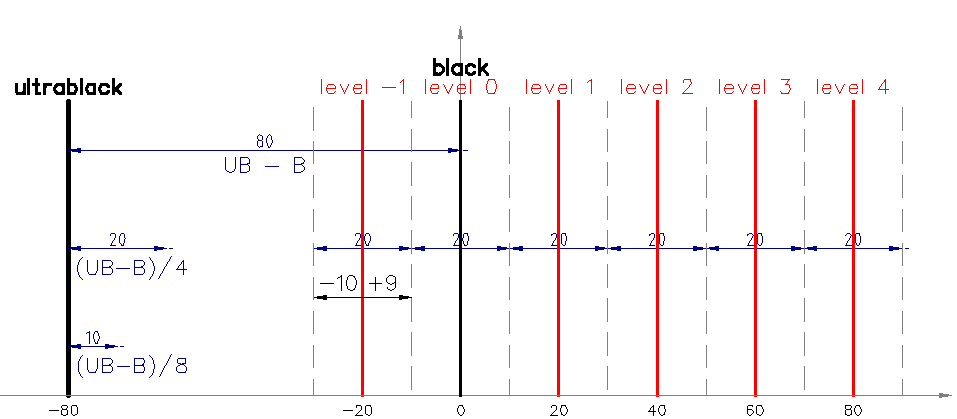
\includegraphics[width=0.95\textwidth]{decode}
	\caption{Schematic of the decoding. The red lines correspond to the ideal position of the level derived from the \ac{UB} and \ac{B}. If a measured value lies in between two dashed grey lines it will be decoded as that level.}
	\label{p15}
\end{figure}

% ========================================================
% 3
% ========================================================
\section{Pattern Generator}
The \ac{PG} is able to send out each of the four commands to the \ac{ROC}: a trigger, a  
\begin{wrapfigure}{r}{3.5cm}
	\includegraphics[width=3.4cm]{PG}
	\caption{example sequence of the \ac{PG}, CC stands for clock cycle}
	\label{p14}
\end{wrapfigure} 
token, a calibrate or a reset. A calibrate will sent out a calibration pulse to the \ac{ROC} and the reset basically deletes all hit information on the \ac{ROC}. It has a register bank with $256$ addresses at its disposal and each of these addresses can hold a single of the four commands and a delay. In that fashion there may be created arbitrary sequences of the four commands. Once the delay is set to $0$ the \ac{PG} will recognise this as a stop sign an ignore the rest of the sequence. An example is shown in \ar{p14}. This would be a basic set-up to test the functionality of the pixels. After a reset to delete all former hit information a calibrate is sent out. To read out the this event, the delay between trigger and calibrate has to be set to \textit{wbc}$+6$ to compensate for the duration the trigger needs to get to the \ac{ROC}. As the final step, the token is send out to collect the data.
% ========================================================
% 4
% ========================================================
\section{Python Interface}
Using cython most of the pXar-core functions are also accessible via python. All the available functions are listed in the cython header file \linebreak[4] ``PyPxarCore.pxd''. Should a function be amiss, it can be added to the header and the source file ``PyPxarCore.pyx`` just like in C++. So that the changes can come into effect and to use the PyPxarCore file the whole program has to be recompiled with the option ``python''.\\
Once that is done the already existing python \ac{CLI} interface ''cmdline.sh`` can be started, which initialises the \ac{DUT} in the same fashion as pXar would do it and allows to program and readout the \ac{DUT} with \ac{API}'s functions.
% ========================================================
% 4
% ========================================================
\section{Running the Software}
Once the software is properly installed meeting all the prerequisites, pXar needs a few configuration files to get started. For each \ac{ROC} that is connected to the \ac{DTB} pXar requires a file called ''dacParameters\_C$<$\ac{I2C}$>$.dat`` with all available \ac{DAC}s and corresponding start values for the respective \ac{ROC} and a file ''trimParameters\_$<$\ac{I2C}$>$.dat`` with a trim bit value for each pixel. If a completely untrimmed \ac{ROC} is required, all values have to be set to $15$, i.e. no trimming at all. Furthermore a file with delay settings for the \ac{DTB} called ''tbParameters.dat`` and a general configuration file ''configParameters.dat`` are required. Examples of these can be found in the appendix \ac{makelink}.\\
All the above files are mandatory to start the software and have to be in the same location (configuration directory). The binary files of pXar are in the directory bin of the installation folder. To run the software one has to go there and enter the command:
\begin{itemize}
	\item[$>$] ./pXar -d $<$configuration directory$>$
\end{itemize}
There are some further useful options to start the program that can be displayed using the ''-h`` option, but it will not start without ''-d``. To name the most important:
\begin{itemize}
	\item -f $<$flashfile$>$ \ka $\rightarrow$ flash a firmware from the flashfile to the \ac{FPGA} of the \ac{DTB}
	\item -g \ka $\rightarrow$ directly starts the \ac{GUI}
\end{itemize}
Since the software will start in a rather undocumented \ac{CLI} if started without the \ac{GUI} option, I recommend starting it always with the ``-g'' option as well.\\
For using the much more user specific \ac{CLI} I was always using the python version, which can be found in the python folder of the installation directory and starts with:
\begin{itemize}
	\item[$>$] ./cmdline.sh -d $<$configuration directory$>$
\end{itemize}
and is very powerful for performing and composing short tests and directly using the \ac{API} commands.
% ========================================================
% 5
% ========================================================
\section{EUDAQ}
EUDAQ is a \ac{DAQ} framework that was designed to be portable, modular and cross platform and was written in C++. It was mainly developed for the EUDET Pixel Telescope, but is very useful for other systems as well \cite{eudaq}. The program is split into different sub processes that can all run on different machines using \ac{TCP} sockets, which are shown in \ar{p16}.\\
The Run Control behaves like a central supervisor of the \ac{DAQ} and shows all the other connected processes, which is why it is the only process that has to run. All the hardware that is connected, e.g. the telescope, a \ac{TU} or other \ac{DUT}s, will have a Producer process and are thereby able to be configured, read out and to send the data to the Data Collector. The Data Collector collects the data from all Producers, combines it to a single data stream and saves it to native binary format. To keep track of potential errors there is also a Logger available that receives log messages from all processes, may receive messages from the user via the Run Control as well and saves the data in single location.\\
Thus, the reason for us using EUDAQ is quite obvious. It makes it very easy to use events off different producers and combine them into one data stream. Though there is still the urge for a trigger logic (q.v. \ar{makeref}) to keep all the events aligned. For the future the idea is to run with another Producer called \ac{TU} that can be configured in the same way as the whole trigger logic.\\
Being independent software, EUDAQ still uses the pXar-core library to operate the telescope.
\begin{figure}[ht]
	\includegraphics[width=0.95\textwidth]{eudaq}
	\caption{Schematic of the EUDAQ architecture \cite{eudaq}.}
	\label{p16}
\end{figure}

\chapter{The Reconnaissance of the Unknown - Experimental Matters}
% \tableofcontents
% ========================================================
% DIGITAL READOUT
% ========================================================
\section{Digital Readout of the Analogue Chip}
Initially the analogue chips were read out with an \ac{ATB} and a software called ``psi46expert''. As already mentioned in \ar{sdtb} the \ac{DTB} has some advantages compared to the \ac{ATB}, which was the reason for switching to the \ac{DTB} controlled by the pXar core libraries. In order to be able to accomplish that, an extension to the pXar core was added by the pXar community that is able to process the data of the analogue \ac{ROC}. The extension includes the decoder described in \ar{sdec} and adds all missing \ac{DAC}s to the library. In addition it utilises the \ac{ADC} of the \ac{DTB}.
% ========================================================
\subsection{Functioning Check}
In order to read out an analogue chip with the \ac{DTB}, first of all the basic functioning should be checked. One has to ascertain that the \ac{DUT} is working\footnote{Working in this context means that it is possible to successfully readout calibrate signals} and that is has a set of appropriate \ac{DAC}s for an analogue \ac{ROC}. For the test board parameter file it is best to use the following lines which were found to be good starting values for the \ac{DTB}:\s
{\ubuntu
\begin{tabular}{llr}
	0	&   clk	&  4\\
	1	&	ctr	&  4\\
	2	&	sda	&  19\\
	3	&	tin	&  9
\end{tabular}}\no\s
For the other necessary files the default files from the Perl script (q.v. \ar{srunpx}) suffice. In the next step the python \ac{CLI} can be started; using the version ``CLIX.py'' simplifies matters a lot.\\
Once the \ac{CLI} is running it has to be checked that the \ac{ROC} is responding and programmable, which can be done by reading out its analogue supply current:
\begin{itemize}
	\tri getTBia
\end{itemize}
The \ac{ROC} is programmable if the current is roughly around $24\,$mA and bigger than $5\,$mA. If this is not the case the test board setting sda is probably incorrect. To resolve it one has to do a scan \textit{sda} (adding $\pm5$ to all test board settings) and repeat the measurement until the \ac{ROC} draws current.
% ========================================================
\subsection{\ac{DTB} Timing}
Since the analogue to digital conversion from the signal of the chip is done within the \ac{DTB}, the exact time when to start and stop sampling the signal are uncertain. The information of the data stream will arrive some time after the token was sent and will end some time after it was received again. These timings can be set by two internal delays of the test board:
\begin{description}
	\item[tindelay:] The time after the token was sent from the \ac{DTB} to the \ac{ROC}. 
	\item[toutdelay:] The time after the token was received from the \ac{DTB}.
\end{description}
The whole process is illustrated in \ar{pdelays}. In order that the decoder can work properly the data has to start with an \ac{UB} level and has to stop with the pulse height of the last pixel hit\footnote{If there is no pixel information within the data, the last level has to be \ac{LD}}. The delays are independent from the length of the data stream, because this length also determines the time in between tin and tout. 
\subsubsection{Finding the delays}
First of all it has to be guaranteed that the pixels can be read out at all by checking the raw data. In order to see the data at all tindelay has to be short enough and toutdelay has to be long enough, s.t. the data is inside the readout window: $5$ and $20$ were found as good starting values. It is advantageous to look at the pixel with the address $5$ $12$ because it includes all $6$ different address levels.\s
\begin{minipage}{5.5cm}
	\begin{itemize}\ubuntu
		\item[$\triangleright$] set\_tb\_delay tindelay 5
		\item[$\triangleright$] set\_tb\_delay toutdelay 20
	\end{itemize}
\end{minipage}
\schema[close]{\vspace*{1.1cm}}{\schemabox{\ubuntu$\triangleright$\hspace*{2pt} set\_tin\_tout 5 20 \footnotemark[3]}}
\footnotetext[3]{The functions behind the curly brackets are short versions from CLIX.py}
\no\s
\begin{minipage}{4.2cm}
	\begin{itemize}\ubuntu
		\tri maskAllPixels 1
		\tri testAllPixels 0
		\tri maskPixel 5 12 0
		\tri testPixel 5 12 1
	\end{itemize}
\end{minipage}
\schema[close]{\vspace*{2.5cm}}{\schemabox{\ubuntu$\triangleright$\hspace*{2pt} enableOnePix 5 20}}
\no\s
\begin{minipage}{4.2cm}
	\begin{itemize}\ubuntu
		\tri daqStart 
		\tri daqTrigger 1 500
		\tri dawGetRawEvent
		\tri daqStop
	\end{itemize}
\end{minipage}
\schema[close]{\vspace*{2.5cm}}{\schemabox{\ubuntu$\triangleright$\hspace*{2pt} daqRawEvent}}\no\s
An example readout looks like this:
\termi{[-3, -19, -9, -193, -1, 96, -55, 58, 108, 164, 212, 93, -4, -6]}
The values slightly below $0$ in the beginning and the end of the example correspond to the zero line of the analogue signal. In between is the \ac{ROC} header and the pixel information. For this example one would have to increase \textit{tindelay} by $3$ and decrease \textit{toutdelay} by $2$ in order to get ride of the base line values. If the pixel information is missing, the delay of the calibration is probably wrong and one has to shift the \ac{DAC} \textit{caldel} by orders of $10$ in both directions until the information appears.
\begin{itemize}
	\tri \ubuntu setDAC caldel <\textit{n}>
\end{itemize}\no\par
During these tests I noticed that the \ac{PG} was set up 
\begin{wrapfigure}{r}{4cm}
	\vspace*{-10pt}
	\includegraphics[width=3.9cm]{findDelay}
	\caption{Example output of findAnalogueTBdelays.}
	\label{pfinddel}
	\vspace*{-5pt}
\end{wrapfigure} 
incorrectly, as the delay between the calibrate and the trigger was set to a fixed value allowing only a  \textit{wbc} of $100$. I fixed that by making the delay dependent on the \textit{wbc} set in the dacParameter file.\\
Once the data is read out correctly and the pixel information is shown one can start adjusting the test board delays. In order to accomplish that function:
\ubu{findAnalogueTBdelays} 
was implemented, which adjusts them automatically. First of all it will activate a single pixel and mask and disable the rest. Then it will increase tindelay from $5$ until the first word in the data stream has a value lower than $-100$, which usually corresponds to \ac{UB}. Afterwards it will decrease toutdelay starting from $20$ until the last word is bigger than $20$, which corresponds to the \ac{PH}. Finally it will print out and set the correct values. An example of its complete output is shown in \ar{pfinddel}. Raw events now should look like this:
\termi{[-196, 0, 97, -54, 57, 106, 164, 212, 91]} 
In order to permanently save the values and start the \ac{DTB} with them per default the following lines have to be added to the tbParameter.dat file:\s
{\ubuntu
\begin{tabular}{llr}
	247	&   tindelay	&  <\textit{found value}>\\
	248	&	toutdelay	&  <\textit{found value}>
\end{tabular}}\no\s
\begin{figure}[ht]
	\centering
	\includegraphics[width=0.95\textwidth]{tbdelays}
	\caption{Demonstration of the test board delays. The clock is always sampling at the rising edge.}
	\label{pdelays}
\end{figure}\no
% ========================================================
\subsection{Sampling Point of the \ac{ADC}}
As one can see in \ar{pdelays} the analogue signal is no rectangular wave. If two levels with different values follow each other the latter one takes some time until it is stable. This behaviour is illustrated in \ar{pdel2}. That is why it important to shift the sampling point of the \ac{ADC} to a sweet spot where the level is stable. In order to accomplish that, the delay of the internal clock has to be adjusted. A wrong sampling point will shift the current level depending on the previous or following one (depending on the position).\\
To find the best delay I implemented the function:
\ubu{find\_clk\_delay} 
for the \ac{CLI}, which will do the following: First it will activate six special pixels that have level sequences $0\rightarrow 2 \rightarrow 0$, $1\rightarrow 2 \rightarrow 1$, $\hdots$, $5\rightarrow 2 \rightarrow 5$ within their pixel addresses\footnote{E.g. the pixel $0$ $44$ decodes to the address levels $0$ \textbf{$0$ $2$ $0$} $0$.}. It will then measure and average the values of the middle address ($2$) for each of these pixels for all clock delay settings from $0-24$. This setting is equivalent to a delay in units of nanoseconds. The corresponding values are plotted in \ar{psplits}. For low clock settings the value is split depending on the pixel from what it is measured. Then all lines converge until they split again for high clock delays. In order to find the ideal clock setting, the function first calculates the mean of all six values for a fixed delay and then it determines the average deviation from that mean value. The delay with the smallest deviation is considered the best setting. In the end the function will print the best value and lowest deviations. Following values in the tbParameter.dat file have to be changed for starting the \ac{DTB} with these settings:\s
{\ubuntu
\begin{tabular}{llr}
	0	&   clk	&  4\\
	1	&	ctr	&  4\\
	2	&	sda	&  19\\
	3	&	tin	&  9
\end{tabular}}
$\longrightarrow$
{\ubuntu
\begin{tabular}{lll}
	0	&   clk	&  <\textit{found value}>\\
	1	&	ctr	&  <\textit{found value}>\\
	2	&	sda	&  <\textit{found value}> + 15\\
	3	&	tin	&  <\textit{found value}> + 5
\end{tabular}}\no\s
By shifting the clock the token in and token out signal might be sampled in another cycle. To compensate for that one should run 
\begin{itemize}
	\tri \ubuntu findAnalogueTBdelays
\end{itemize}
again. Find\_clk\_delay will plot a histogram of the address levels for the best clock delay setting. If there are only single, well separated peaks, the delay was successfully set as in \ar{padrlev}
\begin{figure}[ht]
	\centering
	\subbottom[Schematic level shift for the addresses $0\rightarrow x\rightarrow2\rightarrow x\rightarrow0$. It drawn excessively for better demonstration. Every single coloured line corresponds to a different pixel address. The red arrow marks inconvenient sampling points as one can see the level splitting up.]{\includegraphics[width=0.47\textwidth]{clkdelay}\label{pdel2}}
	\hfill
	\subbottom[Real level splits measured with the find\_clk\_delay function. The vertical line shows the clock setting with the lowest deviation and the vertical lines demonstrate the decoding window.]{\includegraphics[width=0.47\textwidth]{splits}\label{psplitsreal}}
	\caption{Level splits of the analogue signal.}
	\label{psplits}
\end{figure}\no
\begin{figure}[ht]
	\centering
	\includegraphics[width=0.5\textwidth]{address_lvls}
	\caption{Address level histogram of thousands hits of the pixel $5$ $12$.}
	\label{padrlev}
\end{figure}\no
% ========================================================
% TRIMMING
% ========================================================
\section{pXar Tests}
Once the timing and the sampling point are set up correctly the \ac{ROC}s may be operated with the full pXar software. The \ac{GUI} has some very useful test functions that help optimising the \ac{ROC} \ac{DAC}s. A picture of the \ac{GUI} with all its tests can be found in \ar{pgui}. The most important ones are quickly sketched in the following:
% ========================================================
\subsection{GainPedestal}\label{sgainped}
The GainPedestal test measures the pulse height curves for ten different \textit{vcal} values $[50, 100, 150, 200, 250, 210, 350, 490, 630, 1400]$ for every single pixel and saves them to the file ``phCalibration\_C<\textit{\ac{I2C}}>.dat'' into the dacParameter directory. These values are important for the pulse height calibration of real pixel data.
\begin{figure}[ht]
	\centering
	\includegraphics[width=0.95\textwidth]{gui}
	\caption{pXar \ac{GUI}. The tests are shown in the grey tabs.}
	\label{pgui}
\end{figure}\no
% ========================================================
\subsection{DacDacScan}\label{stornado}
The default DacDacScan test counts how often a single pixel can be read out successfully after sending ten triggers for every combination of of the \ac{DAC}s \textit{vcal} and \textit{vthrcomp}. It plots the result in a two dimensional histogram as shown in \ar{ptornado}. The readout is only working within a region that is roughly shaped like a tornado, which is why the plot is usually referenced as ``tornado plots''. The shape is determined by the difference of time signals  need to get to the comparator and the overall threshold of the pixel. 
\begin{figure}[ht]
	\centering
	\subbottom[Tornado plot of an analogue \ac{ROC}]{\includegraphics[width=0.47\textwidth]{DacDacScan}\label{ptornado}}
	\hfill
	\subbottom[PixelAlive map. On the top edge are few pixels that do not work at all. Except from that all pixel have 10/10 readouts.]{\includegraphics[width=0.47\textwidth]{pixmap}\label{ppixmap}}
	\caption{Two pXar tests.}
	\label{ppxartest}
\end{figure}\no
% ========================================================
\subsection{PixelAlive}
The PixelAlive test shows the efficiency of every pixel for ten readouts, checks if every pixel can be masked and if the address decoding works properly. This test is very powerful to quickly inspect the functionality of the readout. An example for a pixel map is shown in \ar{ppixmap}.
% ========================================================
\subsection{Pretest}
The Pretest is a combination of tests that is meant to find the best set up of the \ac{ROC} for calibration pulses. Up until now all the tests, which were designed for the digital \ac{ROC}, work the same way for the analogue one. For the pretest a modification had to be done.\\
First of all the tests checks weather the chip is programmable be reading the analogue current. If that succeeds it continues by optimising the analogue current to a value of $24\,$mA with an iterative procedure. The analogue current increases very linearly with \textit{vana}. The iteration makes use of the general slope of that rise and was failing for the analogue chip. That is why measuring points of the function iana(vana) were recorded with the python \ac{CLI} utilising the commands:
\begin{itemize}\ubuntu
	\tri setDAC vana <\textit{value}>
	\tri getTBia
\end{itemize}
The slope was then extracted from the points by means of a linear regression. It was found that the slope of the analogue chip is roughly a magnitude of order smaller than for the digital and amounts to a value of roughly $0.5\,$mA/DAC compared to $6\,$mA/DAC for the digital chip. From this fact can be deduced that the analogue resistivity of the two chips has the same ratio as the two slopes. After making the vana subtest dependent on the chip and setting the correct slopes, the test was working for the analogue chip as well.\\
If from a list of ten pixels any can be read out successfully the test proceeds with a DacDacScan and sets \textit{vthrcomp} $50$ \ac{DAC}s below the upper threshold of the tornado plot. For that value of \textit{vthrcomp} caldel is set to a value closest to the middle of the tornade by minimising the distance to either side. Finally all changed \ac{DAC}s are saved to their respective files. 
% ========================================================
\subsection{Trim}\label{strim}
The Trim test was implemented to unify the response of all pixels by putting them to the same threshold. Due to variations in electronics, every pixel has a slightly different threshold until it starts sending pixel signals to the periphery.\\
There are two \ac{DAC}s and the so called trim bits that were designed to unify the threshold: \textit{vthrcomp} sets a global threshold, the trim bits can be set differently for each pixel and lower the threshold in a $4\,$bit range\footnote{$1111=15$ is equivalent to an offset of $0$ and $0000$ is the maximum offset}. The amount each trim bit corrects is set by the \ac{DAC} $vtrim$. The only input parameter of the test is the threshold in \textit{vcal} units that the \ac{ROC} shall be unified to.\\
In a first step the algorithms measures the thresholds\footnote{Speaking of the threshold always refers to an absolute value. The \ac{DAC} \textit{vthrcomp} is actually an inverted unit. So if the threshold is raised \textit{vthrcomp} is decreased} for each pixel with the fixed target \textit{vcal}. This is achieved by raising the threshold until the signal is vanishing. Since the trim bits can only lower the threshold afterwards, the highest of these thresholds is selected and set as a global common threshold (q.v. \ar{ptrimthresh}).\\
Afterwards that \textit{vthrcomp} value is kept constant and the \textit{vcal} value for each pixel is raised until the pixels starts showing a signal. The pixel with the highest \textit{vcal}, which has the biggest deviation from the global threshold, is selected and all its trim bits set to $0$ (q.v. \ar{ptrimvcal}). That lowers the threshold by the biggest possible amount. In order for that value to be the same as the global threshold \textit{Vtrim} is raised until its threshold \textit{vcal} is equivalent to the target  \textit{vcal}.\\
In a last step the trim bits for each pixel are set, s.t. their \textit{vcal} is also equivalent to the target \textit{vcal}.\\
If the test succeeds all pixels are set to uniform threshold. For the beam tests as well as for diamond pixel chips it is desirable to set the threshold very low, to collect as much data as possible. The lowest values that could be achieved with the test from pXar are shown in \ar{ttrim}. The limiting factors are the time walk of the low signals, which take longer to get to the comparator and the electric noise of the pixels.
\begin{table}[ht]
	\centering
	\begin{tabular}{c|c|c}
		\noalign{\hrule height 2pt}
		\textbf{\ac{ROC}}	& \textbf{\textit{vcal$_{\z{min}}$}} 	& 	\textbf{electrons}	\\\hline
		analogue 						& $40$						&	$2600$				\\
		digital							& $28$						&	$1300$				\\
		\noalign{\hrule height 2pt}
	\end{tabular}
	\caption{Minimim vcal and electron threshold achieved by trimming. The conversion factor can be measured using x-rays. }
	\label{ttrim}
\end{table}
\begin{figure}[ht]
	\centering
	\subbottom[Finding the global maximum threshold. In the example it is set to the threshold of the pixel $25\ 31$.]{\includegraphics[width=0.47\textwidth]{trimthresh}\label{ptrimthresh}}
	\hfill
	\subbottom[Finding the pixel with maximum difference (in vcal units) to the max threshold. In the example pixel $0\ 2$. ]{\includegraphics[width=0.47\textwidth]{trimvcal}\label{ptrimvcal}}
	\caption{Visualisation of the trim process.}
	\label{ptrim}
\end{figure}\no
% ========================================================
% FAST-OR
% ========================================================
\section{Fast-OR Dependencies}\label{sfastor}
The fast-OR signal, which is only available for the analogue chips, is used as trigger for all experiments done during this thesis except when using calibrate signals. That is why it is very important to understand its behaviour in terms of signal shape. The three \ac{DAC}s \textit{vsumcol}, \textit{vnpix} and \textit{vicolor} in combination with the number of hits per \ac{DC} and the total number of hit \ac{DC}s determine the shape. For the experiments it is important to collect every single pixel hit, which is why a constant and reliable signal is desirable. The aforesaid \ac{DAC}s are designed for a self triggering mode. \textit{Vnpix} and \textit{vicolor} are meant to set thresholds for minimum number of hits per \ac{DC} and the minimum number of \ac{DC}s with hits.\\ 
In order to measure the fast-OR signal a single analogue \ac{ROC} was connected to a \ac{DTB} and controlled with the python \ac{CLI}. Single calibrates can be sent with the \ac{PG} by utilising the command:
\begin{itemize}
	\tri \ubuntu daqTrigger 1 500
\end{itemize}
In \ar{pfastor} the dependencies for a single activated pixel are demonstrated. Increasing \textit{vsumcol} starting from $0$ results in a decrease of the bump on left side of the pulse and shifts the falling right edge slightly to the left. $6$ has been found as good working point.\textit{Vicolor} showed the same behaviour as \textit{vnpix} during their variation. There are three different states (q.v. \ar{pvnpix}) of the signal that merge into each other upon certain thresholds. Within roughly two units of the \ac{DAC}s one signal is merged into another. At a final threshold the signal vanishes completely. The measured thresholds are shown in \ar{tfastor}. The largest signal has biggest range and is the on that has to be used as signal for the fast-OR. Any value within its range serves, so $99$ and $40$ were chosen for $vicolor$ and $vnpix$ respectively.\par
\begin{table}[ht]
	\centering
	\begin{tabular}{c|c|c}
		\noalign{\hrule height 2pt}
		\multirow{2}{*}{\textbf{Signal}}	& \multicolumn{2}{c}{\textbf{Range}} 	\\\cline{2-3}
											& \textit{vnpix}	& \textit{vicolor}	\\\hline
		large 								& $\wz\wz0-113$		& $34-255$			\\
		middle 								& $114-122$			& $19-\wz33$		\\
		small 								& $123-127$			& $16-\wz18$		\\
		off 								& $127-255$			& $\wz0-\wz15$		\\		
		\noalign{\hrule height 2pt}
	\end{tabular}
	\caption{Thresholds of \textit{vnpix} and \textit{vicolor}}
	\label{tfastor}
\end{table}
\begin{figure}[ht]
	\centering
	\subbottom[Effect of different \textit{vsumcol}]{\includegraphics[width=0.47\textwidth]{vsumcol}\label{psumcol}}
	\hfill
	\subbottom[Effect of different \textit{vnpix} and \textit{vicolor}]{\includegraphics[width=0.47\textwidth]{vnpix}\label{pvnpix}}
	\caption{\ac{DAC} effects on the fast-OR of a single pixel measured with and oscilloscope (blue lines).}
	\label{pfastor}
\end{figure}\no
With the above \ac{DAC} settings the dependencies of the number of hit pixels and hit \ac{DC}s was surveyed and the basic shape of the fast-OR was measured, which is shown in \ar{phitcols}. If only one pixel is activated its position within the \ac{ROC} is completely irrelevant, all signals look like \ar{m1}. A single hit produces a roughly $25\,$ns long pulse with slowly rising edges and a short plateau of about $280\,$mV. It also makes no difference how many pixels within one \ac{DC} are activated or how many consecutive \ac{DC}s were hit, the outgoing signal still looks like a single pixel hit. However, the signal begins to change if more than one non-consecutive\footnote{In this context non-consecutive means that one hit \ac{DC} is followed by a number of non hit \ac{DC}s until another \ac{DC} is hit.} \ac{DC} is hit. If this is the case, a second pulse is slowly rising within the rising edge of the single hit signal. For every additional non-consecutive hit \ac{DC} the bump gets bigger until it gets stable at $11$ hits. The second pulse is merging with the first one which lengthens the overall signal just a few nanoseconds, but increases the rising slope a lot. The signal is aside from that almost independent from the total number of hit pixels Yet when more than approximately $87\,$\% of all pixels were hit, the signal gets more than twice as long and shows a characteristic double peak (q.v. \ar{pallfast}).\\
Since it is very unlikely that almost the whole \ac{ROC} or a large number of non-consecutive \ac{DC} is hit at the same time. The fast-OR signal can be considered very stable and very reliable. It was also verified that the shape of the fast-OR is not changed by the use of either telescope.
\begin{figure}[ht]
	\centering
	\includegraphics[width=0.52\textwidth]{fastOR/a1}
	\caption{Fast-OR with all pixels activated}
	\label{pallfast}
\end{figure}\no
\begin{figure}[ht]
	\centering
	\subbottom[Single hit pulse, length intersection]{\includegraphics[width=0.31\textwidth]{fastOR/m2}\label{m1}}
	\hfill
	\subbottom[Single hit pulse length]{\includegraphics[width=0.31\textwidth]{fastOR/m1}\label{m2}}
	\hfill
	\subbottom[Single hit pulse height]{\includegraphics[width=0.31\textwidth]{fastOR/m3}\label{m3}}\\
	\subbottom[1 non-consecutive \ac{DC}s]{\includegraphics[width=0.31\textwidth]{fastOR/d1}\label{pd1}}
	\hfill
	\subbottom[2 non-consecutive \ac{DC}s]{\includegraphics[width=0.31\textwidth]{fastOR/d2}\label{pd2}}
	\hfill
	\subbottom[3 non-consecutive \ac{DC}s]{\includegraphics[width=0.31\textwidth]{fastOR/d3}\label{pd3}}\\
	\subbottom[4 non-consecutive \ac{DC}s]{\includegraphics[width=0.31\textwidth]{fastOR/d4}\label{pd4}}
	\hfill
	\subbottom[5 non-consecutive \ac{DC}s]{\includegraphics[width=0.31\textwidth]{fastOR/d5}\label{pd5}}
	\hfill
	\subbottom[6 non-consecutive \ac{DC}s]{\includegraphics[width=0.31\textwidth]{fastOR/d6}\label{pd6}}\\
	\subbottom[7 non-consecutive \ac{DC}s]{\includegraphics[width=0.31\textwidth]{fastOR/d7}\label{pd7}}
	\hfill
	\subbottom[8 non-consecutive \ac{DC}s]{\includegraphics[width=0.31\textwidth]{fastOR/d8}\label{pd8}}
	\hfill
	\subbottom[9 non-consecutive \ac{DC}s]{\includegraphics[width=0.31\textwidth]{fastOR/d9}\label{pd9}}\\
	\subbottom[10 non-consecutive \ac{DC}s]{\includegraphics[width=0.31\textwidth]{fastOR/d10}\label{pd10}}
	\hspace*{0.45cm}
	\subbottom[11 non-consecutive \ac{DC}s]{\includegraphics[width=0.31\textwidth]{fastOR/d11}\label{pd11}}
	\caption{Fast-OR dependency on hit pixels and \ac{DC}s measured with an oscilloscope. The blue and the yellow line are the two differential signals of the fast-OR.}
	\label{phitcols}
\end{figure}\no
% ========================================================
% WBC Scan
% ========================================================
\section{WBC Scan}
The \textit{wbc} is a very important value for external triggering. Only if it is set to the exact time in clock cycles that the trigger takes to get to the \ac{ROC} after it was hit the \ac{ROC} will release the hit information. Originally it was very laboriously to find correct value. Using the old telescope every plane was set to a different \textit{wbc} until one of them showed hits in the beam. That is why an easier scan using the python \ac{CLI} was implemented.\\
It could be accomplished using the set-up with a single plane and the the radioactive beta source \chemfig{Sr^{90}} under the application of the trigger logic in \ar{striglog1}. The function 
\ubu{wbcScan [min\_wbc=90] [max\_trig=50] [max\_wbc=130]}
automatically finds the \textit{wbc} for an arbitrary number of chips connected to the \ac{DTB}. It also delivers information about the efficiency of each single chip and the relative phase of the trigger compared to the clock. The values in the square brackets are the arguments with their default values. The functionality of the wbcScan is sketched in the following.\par\vspace*{-5pt}
First of all the trigger source of the \ac{DTB} has to be set to ``extern'' to 
\begin{wrapfigure}{l}{5cm}
	\vspace*{-10pt}
	\includegraphics[width=4.9cm]{wbcscan1}
	\caption{Exemplary output of the wbcScan}
	\label{pwbc1}
	\vspace*{-5pt}
\end{wrapfigure} switch to external triggers. Afterwards a new \ac{DAQ} session is started and function starts looping over all \textbf{wbcs} from \textit{min\_wbc}. For every loop it reads out \textit{max\_trig} events and counts the events that have at least one pixel hit in any of the chips (basic yield) as well as the events with at least one pixel hit for every single plane. If the basic yield exceeds $90\,$\% the loop will collect the data for three more \textbf{wbcs} before it stops. Otherwise it will loop over all \textit{wbc}s until \textit{max\_wbc}. After the function is done with looping it will select and set the \textit{wbc} with the highest basic yield and plot a graph with all measured values (q.v. \ar{pwbc2}). In the end it measures the trigger phase for $1000$ events, which is an information the \ac{DTB} acquires via sampling trigger and clock signal with the internal $400\,$MHz clock. Thus, there are $10$ possible phases. Finally it will produce a statistic with the yields per \ac{ROC} some values around the best $wbc$ and a statistic of trigger phases that have more than one event, which is shown in \ar{pwbc1}.
\begin{figure}[ht]
	\centering
	\includegraphics[width=0.6\textwidth]{wbcscan2}
	\caption{Plot of the basic yield of wbcScan}
	\label{pwbc2}
\end{figure}\no
% ========================================================
% DYING FAST-OR
% ========================================================
\section{\ac{TBM} problems}\label{stbmprob}
The software \ac{TBM} is completely controlled by the firmware of the \ac{DTB}. Its basic working principle is describe in \ar{stbm}. During the beam test experiments two problems concerning the \ac{TBM} were encountered that are discussed in the following.
% ========================================================
\subsection{Timing of the \ac{TBM} Trailer}
At the begin of the beam test at \ac{DESY} the data could not be read out at all with the pXar core decoder. Looking at the raw data with the \ac{CLI} revealed that pixels get validated but that the end of the last hit was always cut off after the first level. The events looked like this:
\begin{equation*}
	\overbrace{\hspace*{2.2cm}}^{\z{\ac{ROC} header}}\hspace*{2pt}\overbrace{\hspace*{4cm}}^{\z{\nth{1} pixel hit}}\hspace*{4.3cm}
\end{equation*}
\vspace*{-1.1cm}
\termi{[-205, -8, 36, -2, 54, -46, 148, -4, 78, 103]}
The first thought was an inappropriate toutdelay setting, increasing this delay did not change anything. After that the full raw data blob was investigated showing that the \ac{TBM} header was written in the middle of the last pixel hit. In hexadecimal format that looked like\footnote{Every set of 4 hex numbers is equal to one data word of $16\,$bit}:
\begin{equation*}
	\hspace*{0.5cm}\overbrace{\hspace*{1.9cm}}^{\z{\ac{TBM} header}}\hspace*{2pt}\overbrace{\hspace*{2.9cm}}^{\z{\ac{ROC} header}}\hspace*{2pt}\overbrace{\hspace*{5.9cm}}^{\z{\nth{1} pixel hit}}
\end{equation*}
\vspace*{-1.1cm}
\termi{[a019 8001 8f3e 0006 006e 0fd8 0007 0fd3 00d5 00ad 0092}
\begin{equation*}
	\overbrace{\hspace*{5.9cm}}^{\z{\nth{2} pixel hit}}\hspace*{3.7cm}
\end{equation*}
\vspace*{-1.0cm}
\begin{itemize}
 \item[] \terminal{$\hdots$ 0fd4 e000 c001 0077 0044 409e]} 
\end{itemize}
\vspace*{-0.5cm}
\begin{equation*}
	\underbrace{\hspace*{1.9cm}}_{\z{TBM trailer}}\hspace*{5.7cm}
\end{equation*}
The \ac{TBM} header and trailer both consist out of two words, the first word of the header is initiated with an \textit{a} and the first word of the trailer is initiated with an \textit{e} as shown in the example. These points uses the splitter of pXar to cut the whole data stream into single events, which is why the data is cut off too early in this case.\\
The problem could be temporarily fixed by rewriting the splitting so that it will end the event four positions after it recognised the trailer. Now, the data could be read out with pXar, but a decoding issues arose which is shown in \ar{pdecerr}. Only the last plane of a four plane telescope was showing five vertical stripes within the pixel map. Vertical stripes are caused when the second column address (C1) is set to a constant value. Unfortunately the \ac{TBM} trailer was not only at the wrong position but was overwriting the pixel data as well. In order to avoid the decoding error the last hit of every event had to be discarded.\\
The whole problem could be solved by a new firmware of the \ac{DTB}. Apparently the \ac{ADC} of the \ac{DTB} takes twelve clock cycles to digitise the analogue data. Thereby the data was written to late into the \ac{RAM} even though the \ac{TBM} already started writing the trailer. By taking the delay of the \ac{ADC} into account the whole problem vanished be adding a delay to the \ac{TBM} trailer if the \ac{ADC} is used to digitise the data stream.
\begin{figure}[ht]
	\centering
	\includegraphics[width=0.5\textwidth]{decodingerr}
	\caption{Decoding error in a pixel plane.}
	\label{pdecerr}
\end{figure}\no
% ========================================================
\subsection{Vanishing Fast-OR}
Later during the same beam test another severe problem was discovered. Using the new firmware of the \ac{DTB} the fast-OR coincidences of two planes in an electron beam were vanishing shortly after starting to take data. Also the single fast-OR showed a decreasing rate.\\
Taking a closer examination at PSI revealed that fast-OR of a single plane is completely vanishing if is self triggered on the signals of a strong radioactive \chemfig{Sr^{90}} source. However, it was only vanishing if the \textit{wbc} is set correctly and the triggers get validated in the \ac{ROC}. If the \textit{wbc} was off the fast-OR remained unchanged. For correct \textit{wbc} the rate of the fast-OR was decreasing stepwise until it went down to zero. The speed of this process is highly dependent on the rate of the passing beta particles. Sometimes the fast-OR starts reviving after going to zero but then vanished again.\\
The explanation for that behaviour is a token trigger mismatch in the \ac{ROC} periphery and could be verified by a simple experiment. While putting a strong source on top the analogue chip a high rate of random triggers (without tokens) were sent with the \ac{PG}. Due to the high rate of betas and triggers it happens that some triggers coincidentally come at the right \textit{wbc} and validate a hit, which causes the \ac{DC} to freeze. Since there is no token or no reset to free the \ac{DC}, it just remains frozen and will stop sending fast-ORs. Depending on the rate of trigger and source a stepwise decrease of rate can be observed.\\
In order to find out what is causing the mismatch in self-triggering mode, the signals \textit{token in, token out}, \textit{ctr} of the \ac{DTB} and the fast-OR itself were investigated closer. The first three can be made accessible via
\ubu{signalProbe  <\textit{output}> <\textit{signal}>\footnote{Output stands for the LEMO output of the \ac{DTB} (d1, d2, a1, a2) and the signals are tin (token in), tout (token out) and ctr. }}
In some occasions there were two or more tokens for a single trigger. Such an event is shown in \ar{p2tok}. That is exactly what causes the mismatch of the token and trigger count on the \ac{ROC} and vanishing fast-OR. Since the trigger and token counter are $4\,$bit numbers it is possible that they get back in sync after a while, which explains the revival.\\
The reason for that could be found inspecting the internal signals of the \ac{DTB} even further. It is possible to send almost every signal that used by the \ac{FPGA} so a pin on the \ac{PCB} of the \ac{DTB} where they can be read out with a digital probe of an oscilloscope. By looking at the internal asynchronous trigger signal, which is a logic signal made from external trigger input of the \ac{DTB}, it was conspicuous that the signal was too long in some occasions. Usually it should be exactly one clock cycle but every time multiple token showed up, this signal was lengthened by the amount of additional tokens. Both the asynchronous trigger and the token in are sampled with internal signals called start and stop. These signal are identical and are generated via the internal $400\,$Mhz and $80\,$Mhz clocks and are shown in \ar{pstop}. The asynchronous trigger is generated if the external trigger that is sent to the \ac{DTB} coincides with the start signal and is stopped with any stop signal, which why it should be exactly one clock cycle long. For every time the start signals coincides with the asynchronous trigger the \ac{TBM} sends a token. So if the asynchronous signal is longer than one clock cycles multiple tokens are sent.\\
By looking at stop signal the main cause for the whole problem could be found. It was not continuous but sometimes single pulses were just missing. If a single pulse was missing when the asynchronous trigger should be stopped, the trigger gets too long and is stopped at the next available stop pulse, shown in \ar{ptriglong2}.\\
The solution was lying in the generation of the stop/start signal, which was done if both clocks have a positive edge. If the clock would just go minimal out of sync it could happen, that this operation would not work. By fixing that signal, the whole problem could be solved.
\begin{figure}[ht]
	\centering
	\includegraphics[width=0.6\textwidth]{doubletoken}
	\caption{Measurement of the signals: \ac{CTR} (yellow), discriminated fast-OR (cyan), token in (magenta), token out (green)}
	\label{p2tok}
\end{figure}\no
\begin{figure}[ht]
	\centering
	\subbottom[Generation of the start/stop signal.]{\includegraphics[width=0.6\textwidth]{stopsig}\label{pstop}}\\
	\subbottom[Functioning asynchronous trigger.]{\includegraphics[width=0.8\textwidth]{triglong1}\label{ptriglong1}}\\
	\subbottom[Too long asynchronous trigger.]{\includegraphics[width=0.8\textwidth]{triglong2}\label{ptriglong2}}\\
	\caption{\ac{DTB} signals}
	\label{psigdtb}
\end{figure}\no
% ========================================================
% CLI TESTS
% ========================================================
\section{\ac{CLI} Test Implementations}
% ========================================================
% DIA SHADOW
% ========================================================
\section{Finding \ac{DUT} Shadows}
For using diamond pad detectors as \ac{DUT}s it is
\begin{wrapfigure}{r}{5cm}
	\vspace*{-10pt}
	\includegraphics[width=4.9cm]{diashadow}
	\caption{The hit map of analogue pixel plane while triggered on the signal of a diamond pad.}
	\label{pdiashodow}
	\vspace*{-5pt}
\end{wrapfigure} 
important to spatially align the pads, which are only $4\times4\,$mm, within the planes of the telescopes. The following method describes how that can be accomplished.\\
For the method to work at all, the pads have to roughly aligned to the \ac{ROC}s by eye, s.t. at least a tiny fraction of them overlaps relatively to the beam. Then the trigger output of the a DRS4 evaluation board, which is connected to the pads, is used as external trigger for the telescope planes. The DRS4 has to be set up, s.t. it triggers on one of the channels the pads are connected to. With that trigger the wbcScan has to be used to find the correct wbc for the planes. Finally, data can be collected with the telescope that only shows events where the pad had a signal that triggered the DRS4. The result is shown in \ar{pdiashodow}.\\
Using this method, the pad can be placed very accurately relative to the pixel planes. It can be applied for any \ac{DUT} that can be triggered on.
% ========================================================
% OPTIMISE TRIG WINDOW
% ========================================================
\section{Optimisation of the Trigger Window}
% ========================================================
% EUDAQ AND TLU
% ========================================================
\section{Implementation of EUDAQ and \ac{TLU}}
EUDAQ is a data-taking software that is perfect for handling several, independent data streams and aligning them into single events. It was adapted for a beam test set-up for the telescope by the CMS group at \ac{ETH}.
The general beam test configuration was running on three computers and is sketched in the following:
\begin{itemize}
	\item A laptop inside the beam area was running:
		\begin{itemize}
			\item a DRS4 producer, which handles the data and the configuration of a DRS4 board
			\item a cmspixel producer, which handles the configuration the and data of a \ac{DTB}, using the pXar core libraries
			\item a \ac{TLU} producer, which handles the configuration of the \ac{TLU} 
		\end{itemize}
	\item An accessible computer for data-taking running:
		\begin{itemize}
			\item the Run Control
			\item the Logger
		\end{itemize}
	\item A data server for saving the data running:
		\begin{itemize}
			\item the Data Collector
		\end{itemize}
\end{itemize}
Depending on which \ac{DUT}s are to be examined, the configuration of the producers connected to the laptop may vary.
% ========================================================
\subsection{Masking}\label{smasking}
Masking is a very important feature for the CMS pixel detectors. A masked pixel will not send any information to the periphery of the \ac{ROC}. Not only the noisy or malfunctioning pixels can be disabled but it is very powerful to control the effective trigger area. That means by masking certain areas of the pixels chips it is possible to use only triggers of specific position or arrangement of pixels. That is, for example, very useful if \ac{DUT}s with smaller areas than the pixel chip are examined.\\
For that reason masking was implemented into the cmspixel producer using the commands from the pXar core library. Each pixel of each pixel may be masked by reading in a configuration file that has to contain the information shown in \ar{tmask}. An example of a masked area of a pixel chip is shown in \ar{pmask}.
\begin{figure}[ht]
	\centering
	\includegraphics[width=0.6\textwidth]{mask}
	\caption{Example of partly masked pixel chip, the pixels in white area are masked and thus do not send any hits.}
	\label{pmask}
\end{figure}\no
\begin{table}[ht]
	\begin{tabularx}{\textwidth}{l|c|c|c|X}
		\noalign{\hrule height 2pt}
		\textbf{name}	&		\textbf{I2C}		&		\textbf{col}			&		\textbf{row}		&	\textbf{explanation}						\\\hline
		pix		&	$	0	$	&	$	12	$	&	$	36	$	&	mask pixel in col 12 and row 36 of I2C 0			\\	
		row		&	$	1	$	&	$	10	$	&	$	20	$	&	mask row 10-20 (including 10 and 20) of I2C 1		\\
		row		&	$	2	$	&	$	10	$	&	$	10	$	&	mask row 10 of I2C 2								\\
		col		&	$	3	$	&	$	14	$	&	$	30	$	&	mask col 14-30										\\
		roc		&	$	4	$	&				&				&	mask the whole ROC of I2C 4							\\
		cornBot	&	$	0	$	&	$	\wz5$	&	$\wz7	$	&	\multirow{2}{7.5cm}{leaves a box with the lower left corner (5/7) to the upper right corner (12/10) unmasked, i.e. row col 5-12 and row 7-10.}	\\
		cornTop	&	$	0	$	&	$	12	$	&	$	10	$	&														\\
		&&&&\\
		\noalign{\hrule height 2pt}
	\end{tabularx}
	\caption{Examplary masking commands.}
	\label{tmask}
\end{table}
% ========================================================
% PULSE HEIGHT CAL
% ========================================================
\section{Pulse Height Calibration}\label{spulseheight}
In order to draw conclusions about the energy of the particles that pass through the detector, the number of created electron-hole pairs is required. Utilising the information of the GainPedestal test of \ar{sgainped} the pulse height vs. \textit{vcal} points are fitted with an error function using ROOT.
\begin{itemize}
	\item[] $[3]^{*}(\z{TMath}::\z{Erf}((x-[0])/[1]+[2])$
\end{itemize}
The error function is converging very well as shown for two examples in \ar{perrfit}. The fit parameters are saved for every \ac{ROC}. With the conversion factor of the vcal into electrons one is able to convert every every measured pulse height into a number of electrons using these fit functions.
\begin{figure}[ht]
	\centering
	\subbottom[Pixel 14 14]{\includegraphics[width=0.47\textwidth]{errfit1}\label{perrfit1}}
	\hfill
	\subbottom[Pixel 26 51]{\includegraphics[width=0.47\textwidth]{errfit2}\label{perrfit2}}
	\caption{Fits of the pulse height vs. \textit{vcal} function for two random pixels.}
	\label{perrfit}
\end{figure}\no
% ========================================================
\label{sexp}
\chapter{The Investigation of the Accumulations - Analysis}
This chapter grants a little insight in the analysis of the data taking with COCPITT. Due to lack of time not all of the analysis that was done during this thesis is explained here. All the things that were also done but are not further described in the thesis are named in the following:
\begin{itemize}
	\item The Investigation of events with large amounts of hits (delta rays)
	\item A study of the leakage current of the silicon sensors and diamond sensors. That included a self implemented software to control the power supplies and to log the measurement as well as a self implemented software to read out the log files and plot the information.
	\item A software to read out the log files from EUDAQ.
\end{itemize}
It was also planned to estimate a resolution of the telescope.
% ========================================================
% TELESCOPE
% ========================================================
\section{Telescope Analysis}
The analysis for COCPITT is based on an existing C++ software called TrackingTelescope that was implemented for the \ac{PLT}. This software was adapted and optimised for the new telescope. It was reorganised by splitting it into several classes, and different file readers were implemented to work with the data of both \ac{PLT} and COCPITT. Furthermore some analysis functions were improved and the whole output in form of histograms and graphs was reworked adding additional features.\\
The software needs a ROOT tree containing the pixel data as input, that requires branches with vectors containing the information of the hits within the telescope: event number, time, plane, col, row and adc. This file can be generated from the raw binary format that EUDAQ is saving by the Converter.exe of EUDAQ:
\ubu{\textit{eudaq-directory}/bin/Converter.exe -t drs4tree <\textit{binary data file}>}
The analysis tools are explained in the following subsections. All the information shown comes from the beam test of October 2015 at \ac{PSI} and was recorded with EUDAQ and version 2 of COCPITT.
% ========================================================
\subsection{Coordinate system}
When speaking of coordinates in the following, the $z-$axis is always referring to the beam axis, the $x-$axis to the horizontal axis perpendicular to the beam and the $y-$axis to the vertical axis.  The $x-y$ plane is is parallel to the pixel detectors and $x$ and $y$ are more or less aligned to the columns and the rows of the chips. The local coordinate system is the coordinate system for each single plane and the telescope coordinate system the a global one for all planes.
% ========================================================
\subsection{Hit Map}
The software is looping over every single event and creates a Hit object for every pixel hit in the event. These Hit objects contain information about the \ac{ROC}, the columns, the row and the \ac{PH}. Hit maps are then generated for every \ac{ROC} by filling a 2D histogram with the column and row information. These histograms show how often each pixel of a \ac{ROC} was hit during the whole event (\ar{phitmap}).
\begin{figure}[ht]
	\centering
	\subbottom[Analogue plane 1 , partly masked]{\includegraphics[width=0.47\textwidth]{hitmap1}\label{phitmap1}}
	\hfill
	\subbottom[Analogue plane 2 , partly masked]{\includegraphics[width=0.47\textwidth]{hitmap2}\label{phitmap2}}
	\caption{Hitmaps of run $313$}
	\label{phitmap}
\end{figure}\no
% ========================================================
\subsection{Alignment}
A particle crossing the telescope generates hits within the telescope, with that information one tries to reconstruct the track of the passing particle. In order to reconstruct the track as good as possible the positions of each plane relative to each other must be known as good as possible. In reality the planes are not aligned perfectly due to indifferent mountings or even badly aligned if different types of planes are used together. In the alignment one uses multiple tracks of particles to find the spatial offsets in $x$ and $y$ and the rotation angle in phi of each plane.\\
First of all, special events have to be selected that can be used for tracking, because tracking gets more accurate the more points are used. In order to select those events, the hits of every event are grouped together to clusters. If the particle creates a lot electrons in the sensor or the sensor is hit close to the border between pixels, the charge can be shared between a couple of pixels. Therefore hits in consecutive pixels are put into a cluster whose centre is weighted by the amount of charge in each pixel. Only events with exactly one cluster in each plane are selected for the alignment.\\
The $z$ position of each plane is precisely measured with a solid gauge and is fixed, since the precision of the alignment in $z$ direction is not that good. Looping over all tracks and employing an iterative algorithm that uses the plane closest to beam as reference, the other planes are first rotated around the $z$-axis and then translated in $x$ and $y$ direction until the residuals of the tracks are minimal. In order to do that, it needs the relative $z-$position of the planes as input. The rotation angle and the two translations are then saved for every plane and can be used in the following. 
% ========================================================
\subsection{Tracking}
In a first step all hits are aligned using the rotation angle and the translations from above. Also for the tracking only events are used that have a single cluster in each plane. Then the points of the cluster centres are fitted using linear regression with errors that are rated with the digital resolution of $1/\sqrt{12}\,$pixelsize. It is possible to use the extracted residuals to get a better estimate for the errors, s.t. they can be adjusted for each pane separately.\\
Using the informations of the fit, the slope of the $x-$ and $y-$projections of the tracks is filled into a histograms, which are then fitted by a Gaussian to measure the centre. Examples of these histograms are illustrated in \ar{pslope}. If the slope distribution is not centred around the zero the planes are not perpendicular to the beam. That is why this information can be used to physically align the telescope to the beam. Furthermore the $\upchi^{2}$ for both projections as well as for the track are filled into histograms as well. The $\upchi^{2}$ is good indicator for the quality of the tracks and can be used as selection criterion for further analysis. Examples of these histograms are shown in \ar{pchi}.
The software will also plot an event display for selected events of every run that shows the path of the track and hits in each plane, as well as a 3D illustration of the track. This is depicted in \ar{pevent} and \ar{p3D}.\\
In order to check the alignment the distributions of the residuals for each plane is drawn. Examples are shown in \ar{pres}.
\begin{figure}[ht]
	\centering
	\subbottom[Slope of the $x$-projection.]{\includegraphics[width=0.47\textwidth]{tracking/slopex}\label{pslope1}}
	\hfill
	\subbottom[Slope of the $y$-projection]{\includegraphics[width=0.47\textwidth]{tracking/slopey}\label{pslope2}}
	\caption{Track slopes of run $313$.}
	\label{pslope}
\end{figure}\no
\begin{figure}[ht]
	\centering
	\subbottom[$\upchi^{2}$]{\includegraphics[width=0.31\textwidth]{tracking/chi}\label{pchia}}
	\hfill
	\subbottom[$\upchi^{2}$ of the $y$-projection]{\includegraphics[width=0.31\textwidth]{tracking/chix}\label{pchi1}}
	\hfill
	\subbottom[$\upchi^{2}$ of the $y$-projection]{\includegraphics[width=0.31\textwidth]{tracking/chiy}\label{pchi2}}
	\caption{$\upchi^{2}$s of run $313$.}
	\label{pchi}
\end{figure}\no
\begin{figure}[ht]
	\centering
	\subbottom[Residual in $x$.]{\includegraphics[width=0.47\textwidth]{tracking/resx}\label{pres1}}
	\hfill
	\subbottom[Residual in $y$.]{\includegraphics[width=0.47\textwidth]{tracking/resy}\label{pres2}}
	\caption{Residual of plane $0$ of run $313$.}
	\label{pres}
\end{figure}\no
\begin{figure}[ht]
	\centering
	\includegraphics[width=0.95\textwidth]{tracking/event}
	\caption{Event display for an event of run $313$ including the fit}
	\label{pevent}
\end{figure}\no
\begin{figure}[ht]
	\centering
	\includegraphics[width=0.5\textwidth]{tracking/3D}
	\caption{3D track display for an event of run $313$ including the fit}
	\label{p3D}
\end{figure}\no
% ========================================================
% PULSE HEIGHTS
% ========================================================
\subsection{Pulse Heights}
The pulse height provides information of the energy the particle has left inside the sensor. In order to convert the \ac{ADC} values of the data into electrons, the results of the pulse height calibration in \ar{spulseheight} are used. With the help of them the charge of each cluster can be achieved by summing up all charges of its consisting hits. Then The charge of the clusters with one, two ore three and more hits are compared with the distribution of all cluster sizes. Examples for a digital and an analogue chip are shown in \ar{pphmap1} and \ar{pphmap2}\\
For both digital and analogue distributions single hits are dominant and for the digital one the peak of each sub distribution is roughly at the same spot, which is expected. For the analogue though, the distributions of the bigger clusters is shifted to lower energies, which is not yet understood and has to be analysed further. The peaks of the main distributions of digital and analogue \ac{ROC} are roughly at the same energy of $25000$ electrons. Alltogether, the \ac{PH} calibration is working well for the digital chip.\\
As demonstrated in \ar{plandaufit} the signal of the digital chip is nicely landau shaped, as would be expected by theory.\\
By looking at the longer range of the energy in \ar{plong1log} and \ar{plong6log} a second prominent peak shows up at around $120000$ and $170000$ electrons for analogue and digital \ac{ROC} respectively. The \ac{PSI} pion beam consists also a tiny fraction of protons. Since protons are about seven times heavier than pions and the particles are with a momentum of $260\,$MeV/c still in the $1/\beta$ range of the Bethe-formula \ar{ebethe} the proton should lose of the order of $10$ more energy than a pion. Due to that, the second peak should belong to protons and the first one to pions. By looking at the size of the proton peaks one can also see that the total number of protons for the digital chip is an order of ten times smaller then for the analogue \ac{ROC}. In the set-up of the picture the analogue plane was closer to the beam with other planes in between the two. That is why the lower number of protons is expected as they have a higher stopping power, which also means that the protons are more likely to scatter. 
\newpage
\begin{figure}[ht]
	\centering
	\subbottom[analogue \ac{ROC} short scale]{\includegraphics[width=0.47\textwidth]{tracking/ph6}\label{pph6}}
	\hfill
	\subbottom[digital \ac{ROC} short scale]{\includegraphics[width=0.47\textwidth]{tracking/long6log}\label{plong6log}}
	\caption{Pulse height distributions for a digital plane}
	\label{pphmap1}
\end{figure}\no
\begin{figure}[ht]
	\centering
	\subbottom[analogue \ac{ROC} long scale, logarithmic y-axis]{\includegraphics[width=0.47\textwidth]{tracking/ph1}\label{pph1}}
	\hfill
	\subbottom[digital \ac{ROC} long scale, logarithmic y-axis]{\includegraphics[width=0.47\textwidth]{tracking/long1log}\label{plong1log}}
	\caption{Pulse height distributions for an analogue plane}
	\label{pphmap2}
\end{figure}\no
\begin{figure}[ht]
	\centering
	\includegraphics[width=0.65\textwidth]{tracking/landaufit}
	\caption{Landau fit of the cluster charge distribution of a digital \ac{ROC}}
	\label{plandaufit}
\end{figure}\no
% RESOLUTION
% ========================================================
% \section{Resolution}
% % ========================================================
% % DELTA RAYS
% % ========================================================
% \section{Delta Rays}
% % ========================================================
% % KEITHLEY CURRENTS
% % ========================================================
% \section{Keithley Currents}
% % ========================================================
% % LOG READER
% % ========================================================
% \section{EUDAQ Log Reader}
% ========================================================

\chapter{The Consequences of the Undertaking - Conclusions}
This thesis could demonstrate the functioning of COCPITT with all its desired features. It was proven that is possible to read out the analogue CMS pixel chips with a \ac{DTB}. All arising problems could be solved. Due to the digital readout there is in principle no limit for the data-taking any more except the size of a computer's hard drive.\\
It was also shown that the telescope is very flexible and easy to deploy in various environments. It can be used to examine different \ac{DUT}s like diamond pad detectors or digital CMS pixel detectors for example.\\
Furthermore, the telescope delivers a reliable trigger for itself and for the \ac{DUT} that has a freely adjustable trigger area using the ability to mask pixels. Above all it has been demonstrated that COCPITT gathers meaningful information about pulse heights and particle tracks.\\
The goal for the future is a complete table-top set-up of the telescope by replacing replacing the trigger logic by the \ac{TU} of the Ohio State University. That way the telescope will work out of the box with almost no installation time. It is also planned to conduct a study of telescope's resolution exploiting the residual distribution of the particle tracks.
% ========================================================


% ========================================================
% ACRONYMS
% ========================================================
\chapter*{List of Acronyms}
\begin{acronym}[Bash]
	\acro{PUC}{pixel unit cell}
	\acro{ROC}{readout chip}
	\acro{TBM}{token bit manager}
	\acro{UB}{ultra black}
	\acro{B}{black}
	\acro{CMS}{Compact Muon Solenoid}
	\acro{LHC}{Large Hadron Collider}
	\acro{CERN}{European Organization for Nuclear Research}
	\acro{DAC}{digital to analogue converter}
	\acro{ADC}{analogue to digital converter}
	\acro{LD}{last DAC}
	\acro{DTB}{digital test board}
	\acro{ATB}{analogue test board}
	\acro{ETH}{Eidgen{\"o}ssische Technische Hochschule}
	\acro{FPGA}{Field Programmable Gate Array}
	\acro{PSI}{Paul Scherrer Institut}
	\acro{HV}{high voltage}
	\acro{TTL}{Transistor-Transistor-Logic}
	\acro{PLL}{phase-locked loop}
	\acro{FIFO}{First In - First Out}
	\acro{HAL}{hardware abstraction layer}
	\acro{API}{application programming interface}
	\acro{GUI}{graphical user interface}
	\acro{CLI}{command line interface}
	\acro{DAQ}{data acquisition}
	\acro{CPU}{central processing unit}
	\acro{PG}{pattern generator}
	\acro{I2C}[I$^{2}$C]{Inter-Integrated Circuit}
	\acro{DUT}{device under test}
	\acro{TCP}{Transmission Control Protocol}
	\acro{TU}{trigger unit}
	\acro{COM}{centre of mass}
	\acro{PSB}{Proton Synchrotron Booster}
	\acro{PS}{Proton Synchrotron}
	\acro{SPS}{Super Proton Synchrotron}
	\acro{ALICE}{A Large Ion Collider Experiment}
	\acro{ATLAS}{A Toroidal LHC Apparatus}
	\acro{LHCb}{Large Hadron Collider beauty}
	\acro{LHCf}{ Large Hadron Collider forward}
	\acro{TOTEM}{TOTal Elastic and diffractive cross section Measurement}
	\acro{SUSY}{supersymmetry}
	\acro{HCAL}{hadronic calorimeter}
	\acro{ECAL}{electromagnetic calorimeter}
	\acro{CTR}{calibrate trigger reset}
	\acro{MIP}{minimum ionising particle}
	\acro{PM}{photo multiplier}
	\acro{TLU}{trigger logic unit}
	\acro{PH}{pulse height}
	\acro{DC}{double column}
	\acro{DESY}{Deutsches Elektronen-Synchrotron}
	\acro{RAM}{Random-Access Memory}
	\acro{PCB}{printed circuit board}
	\acro{PLT}{Photo Luminosity Telescope}
	\acro{RPC}{remote procedure calls}
\end{acronym}
% ========================================================
% APPENDIX
% ========================================================
\appendix
\chapter{Appendix}
\section{Applied Software}\label{ssoft}
The master branch of pXar and the branch that used during the thesis can be downloaded from git: 
\begin{itemize}
	\item \url{https://github.com/psi46/pxar}
	\item \url{https://github.com/michareichmann/pxar}
\end{itemize}
More information as well a detailed installation instruction can be found at the \ac{CMS} twiki: 
\begin{itemize}
	\item \url{https://twiki.cern.ch/twiki/bin/viewauth/CMS/Pxar} $rightarrow$ branch eth-2.0
\end{itemize}
The version of EUDAQ that was used can be found here: 
\begin{itemize}
	\item \url{https://github.com/veloxid/eudaq-drs4}. 
\end{itemize}
\section{Example Configuration Files}\label{sconfig}
\subsubsection{dacParameters\_C1.dat}
\ubuntu
\begin{tabular}{llr}
\hline
1	&	vdig	&	6	\\
2	&	vana	&	119	\\
3	&	vsh	&	140	\\
4	&	vcomp	&	10	\\
5	&	vleak	&	0	\\
6	&	vrgpr	&	0	\\
7	&	vwllpr	&	35	\\
8	&	vrgsh	&	0	\\
9	&	vwllsh	&	35	\\
10	&	vhlddel	&	160	\\
11	&	vtrim	&	100	\\
12	&	vthrcomp	&	101	\\
13	&	vibias\_bus	&	30	\\
14	&	vbias\_sf	&	10	\\
15	&	voffsetop	&	30	\\
16	&	vibiasop	&	50	\\
17	&	phoffset	&	120	\\
18	&	vion	&	130	\\
19	&	vcomp\_adc	&	120	\\
20	&	phscale	&	109	\\
21	&	vibias\_roc	&	150	\\
22	&	vicolor	&	99	\\
23	&	vnpix	&	40	\\
24	&	vsumcol	&	6	\\
25	&	vcal	&	255	\\
26	&	caldel	&	140	\\
253	&	ctrlreg	&	4	\\
254	&	wbc	&	100	\\\hline
\end{tabular}
\subsubsection{tbParameters.dat}
\ubuntu
\begin{tabular}{llr}
\hline
0	&	clk	&	12	\\
1	&	ctr	&	12	\\
2	&	sda	&	24	\\
3	&	tin	&	14	\\
4	&	tout	&	5	\\
252	&	level	&	15	\\
247	&	tindelay	&	14	\\
248	&	toutdelay	&	8	\\
251	&	triggerlatency	&	80	\\
254	&	deser160phase	&	4	\\\hline
\end{tabular}
\subsubsection{configParameters.dat}
\ubuntu
\begin{tabular}{llr}
\hline
\multicolumn{2}{l}{-- parameter files}		\\
	&				\\
tbParameters	&	tbParameters.dat			\\
dacParameters	&	dacParameters			\\
tbmParameters	&	tbmParameters			\\
trimParameters	&	trimParameters			\\
testParameters	&	testParameters.dat			\\
maskFile	&	defaultMaskFile.dat			\\
rootFileName	&	pxar.root			\\
	&				\\
\multicolumn{2}{l}{-- configuration}	\\
	&				\\
nModules	&	1			\\
\#nRocs	&	1	i2c:	0,1,2,3,4,5,6,7,8,9,10,11,12,13,14,15	\\
nRocs	&	1	i2c:	1	\\
nTbms	&	0			\\
hubId	&	0			\\
tbmEnable	&	0			\\
tbmEmulator	&	0			\\
hvOn	&	1			\\
tbmChannel	&	0			\\
rocType	&	psi46v2			\\
	&				\\
probeA1	&	sdata1			\\
probeA2	&	sdata2			\\
probeD1	&	clk			\\
probeD2	&	ctr			\\
	&				\\
\multicolumn{2}{l}{-- voltages and current}	\\
	&				\\
ia	&	1.199			\\
id	&	1			\\
va	&	1.699			\\
vd	&	2.5			\\
\hline
\end{tabular}
\subsubsection{trimParameters.dat}
\ubuntu
\begin{tabular}{lllr}
\hline
3	&	Pix	&	0	&	0	\\
2	&	Pix	&	0	&	1	\\
5	&	Pix	&	0	&	2	\\
5	&	Pix	&	0	&	3	\\
4	&	Pix	&	0	&	4	\\
4	&	Pix	&	0	&	5	\\
4	&	Pix	&	0	&	6	\\
5	&	Pix	&	0	&	7	\\
4	&	Pix	&	0	&	8	\\
8	&	Pix	&	0	&	9	\\
8	&	Pix	&	0	&	10	\\
\multicolumn{4}{c}{$\vdots$}\\
\hline
\end{tabular}
% ========================================================

% ========================================================
% BIBLIOGRAPHY
% ========================================================
\backmatter
\bibliographystyle{plain}
\bibliography{compile/refs}
\includepdf[pages={-}]{sections/declaration.pdf}
% ============================
% DOCUMENT END
% ============================
\end{document}

